\noindent In Kapitel 5 wird die z-Transformation von Signalen vorgestellt und an Beispielen vertieft. Die z-Transformation kann zur analytischen L\"{o}sung von Differenzengleichungen mit konstanten Koeffizienten eingesetzt werden. Es wird sich zeigen, dass die analytische L\"{o}sung von Differenzengleichungen mit Hilfe der z-Transformation einfacher und \"{u}bersichtlicher ist als die Vier-Schritt-Methode im Zeitbereich.\newline

\noindent Die L\"{o}sung von linearen Differenzengleichungen f\"{u}hrt zu dem Begriff der \"{U}bertragungsfunktion f\"{u}r zeitdiskrete Systeme. Sie weist Parallelen zur \"{U}bertragungsfunktion zeitkontinuierlicher Systeme auf. Auch die Interpretation der \"{U}bertragungsfunktion ist \"{a}hnlich. So lassen sich zum Beispiel Stabilit\"{a}tsaussagen und Aussagen zur Schwingungsneigung sowie zur Sprungf\"{a}higkeit an der Pollage der \"{U}bertragungsfunktion ablesen. Wesentlich dabei ist, den in Kapitel 5 beschriebenen Zusammenhang zwischen der s- und z-Ebene zu kennen. \newline

\noindent Die Interpretation der unterschiedlichen Systeme f\"{u}hrt zur Einteilung in Systeme mit endlicher und unendlicher Impulsantwort. Aufgrund ihrer Impulsantworten werden sie als Finite-Impulse-Response-Systeme (FIR-Systeme) beziehungsweise Infinite-Impulse-Response-Systeme (IIR-Systeme) bezeichnet. Bei dem Entwurf zeitdiskreter Systeme wird sich zeigen, dass FIR- und IIR-Systeme grunds\"{a}tzlich unterschiedliche Entwurfsverfahren erfordern.\newline

\noindent In der Praxis wird die Simulation und Interpretation zeitdiskreter Systeme mit Programmen wie MATLAB und Simulink durchgef\"{u}hrt. Die dazu erforderlichen Befehle und Methoden werden kurz vorgestellt und an Beispielen verdeutlicht.

\subsection{L\"{o}sung von Differenzengleichungen mit der z-Transformation}

\noindent Differenzengleichungen beschreiben das Verhalten zeitdiskreter Systeme \"{a}hnlich, wie Differentialgleichungen das Verhalten zeitkontinuierlicher Systeme beschreiben. Differenzengleichungen k\"{o}nnen im Zeitbereich gel\"{o}st werden. Das Verfahren dazu wird in Kapitel 0 vorgestellt. Es besteht aus mehreren Schritten und ist insbesondere bei Ber\"{u}cksichtigung von Anfangsbedingungen aufwendig. Eine effizientere M\"{o}glichkeit zur L\"{o}sung von Differenzengleichungen wird mit der z-Transformation erreicht. Das Vorgehen wird in Bild \ref{fig:LoesungDGLImZBereich} skizziert.

\begin{figure}[H]
  \centerline{\includegraphics[width=0.5\textwidth]{Kapitel6/Bilder/image1.png}}
  \caption{Verfahren zur L\"{o}sung von Differenzengleichungen mit der z-Transformation}
  \label{fig:LoesungDGLImZBereich}
\end{figure}

\noindent Die Differenzengleichung wird mit Hilfe der z-Transformation in den z-Bereich transformiert. Aufgrund der Rechenregeln der z-Transformation ergibt sich eine algebraische Gleichung, die im z-Bereich gel\"{o}st wird. Mit Hilfe der R\"{u}cktransformation \"{u}ber Partialbruchzerlegung wird die L\"{o}sung im Zeitbereich bestimmt.

\subsubsection{L\"{o}sung linearer Differenzengleichungen ohne Anfangsbedingungen}

\noindent Zur L\"{o}sung der Differenzengleichung wird von der allgemeinen Form ausgegangen

\begin{equation}\label{eq:sixone}
\sum _{n=0}^{N}c_{n} \cdot y\left[k-n\right] =\sum _{l=0}^{L}d_{l} \cdot u\left[k-l\right]
\end{equation}

\noindent Mit der Verschiebungsregel nach rechts ergibt sich die z-Transformierte der Gleichung zu

\begin{equation}\label{eq:sixtwo}
\sum _{n=0}^{N}c_{n} \cdot Y\left(z\right)\cdot z^{-n}  =\sum _{l=0}^{L}d_{l} \cdot U\left(z\right)\cdot z^{-l}
\end{equation}

\noindent Nach Ausklammern der beiden z-Transformierten Y(z) und U(z)

\begin{equation}\label{eq:sixthree}
Y\left(z\right)\cdot \sum _{n=0}^{N}c_{n} \cdot z^{-n}  =U\left(z\right)\cdot \sum _{l=0}^{L}d_{l} \cdot z^{-l}
\end{equation}

\noindent kann die Gleichung nach der z-Transformierten des Ausgangssignals Y(z) aufgel\"{o}st werden.

\begin{equation}\label{eq:sixfour}
Y\left(z\right)=\frac{\sum _{l=0}^{L}d_{l} \cdot z^{-l}  }{\sum _{n=0}^{N}c_{n} \cdot z^{-n}  } \cdot U\left(z\right)
\end{equation}

\noindent Die L\"{o}sung im z-Bereich ist eine gebrochen rationale Funktion, die mit Hilfe der Partialbruchzerlegung und den bekannten Korrespondenzen in den Zeitbereich zur\"{u}ck transformiert werden kann. Dieses Vorgehen wird an der Differenzengleichung eines rekursiven Tiefpasses verdeutlicht.\bigskip

\noindent
\colorbox{lightgray}{%
\arrayrulecolor{white}%
\renewcommand\arraystretch{0.6}%
\begin{tabular}{ wl{16.5cm} }
{\fontfamily{phv}\selectfont{Beispiel: Rekursiver Tiefpass ohne Anfangsbedingungen}}
\end{tabular}%
}\medskip

\noindent Es soll die Reaktion eines rekursiven Tiefpasses auf einen Sprung der Eingangsgr\"{o}{\ss}e u[k] von der H\"{o}he U${}_{0}$ berechnet werden. Das Eingangssignal besitzt die z-Transformierte

\begin{equation}\label{eq:sixfive}
U\left(z\right)=\frac{z}{z-1} \cdot U_{0}
\end{equation}

\noindent Das \"{U}bertragungsverhalten des rekursiven Tiefpasses wird mit der Differenzengleichung

\begin{equation}\label{eq:sixsix}
y\left[k\right]-GF\cdot y\left[k-1\right]=\left(1-GF\right)\cdot u\left[k\right]
\end{equation}

\noindent beschrieben. Die Transformation der Gleichung in den z-Bereich ergibt

\begin{equation}\label{eq:sixseven}
Y\left(z\right)\cdot \left(1-GF\cdot z^{-1} \right)=\left(1-GF\right)\cdot \frac{z}{z-1} \cdot U_{0}
\end{equation}

\noindent Aufl\"{o}sen nach der z-Transformierten des Ausgangssignals Y(z) f\"{u}hrt zu

\begin{equation}\label{eq:sixeight}
Y\left(z\right)=\frac{z}{z-GF} \cdot \left(1-GF\right)\cdot \frac{z}{z-1} \cdot U_{0}
\end{equation}

\noindent Mit Hilfe der Partialbruchzerlegung kann Y(z) dargestellt werden als 

\begin{equation}\label{eq:sixnine}
Y\left(z\right)=\frac{z}{z-GF} \cdot \left(1-GF\right)\cdot \frac{z}{z-1} \cdot U_{0} =\left(\left(-GF\right)\cdot \frac{z}{z-GF} +\frac{z}{z-1} \right)\cdot U_{0}
\end{equation}

\noindent Die Darstellung mit Partialbr\"{u}chen erm\"{o}glicht die R\"{u}cktransformation in den Zeitbereich zu

\begin{equation}\label{eq:sixten}
y\left[k\right]=\left(\left(-GF\right)\cdot GF^{k} \cdot \sigma \left[k\right]+\sigma \left[k\right]\right)\cdot U_{0} =\left(1-GF^{k+1} \right)\cdot U_{0} \cdot \sigma \left[k\right]
\end{equation}

\noindent Ein Vergleich mit der \"{u}ber die Faltungssumme berechneten Systemantwort in Bild \ref{fig:DifferenzengleichungOhneAnfangsbedingungen} zeigt identische Ausgangssignale.

\begin{figure}[H]
  \centerline{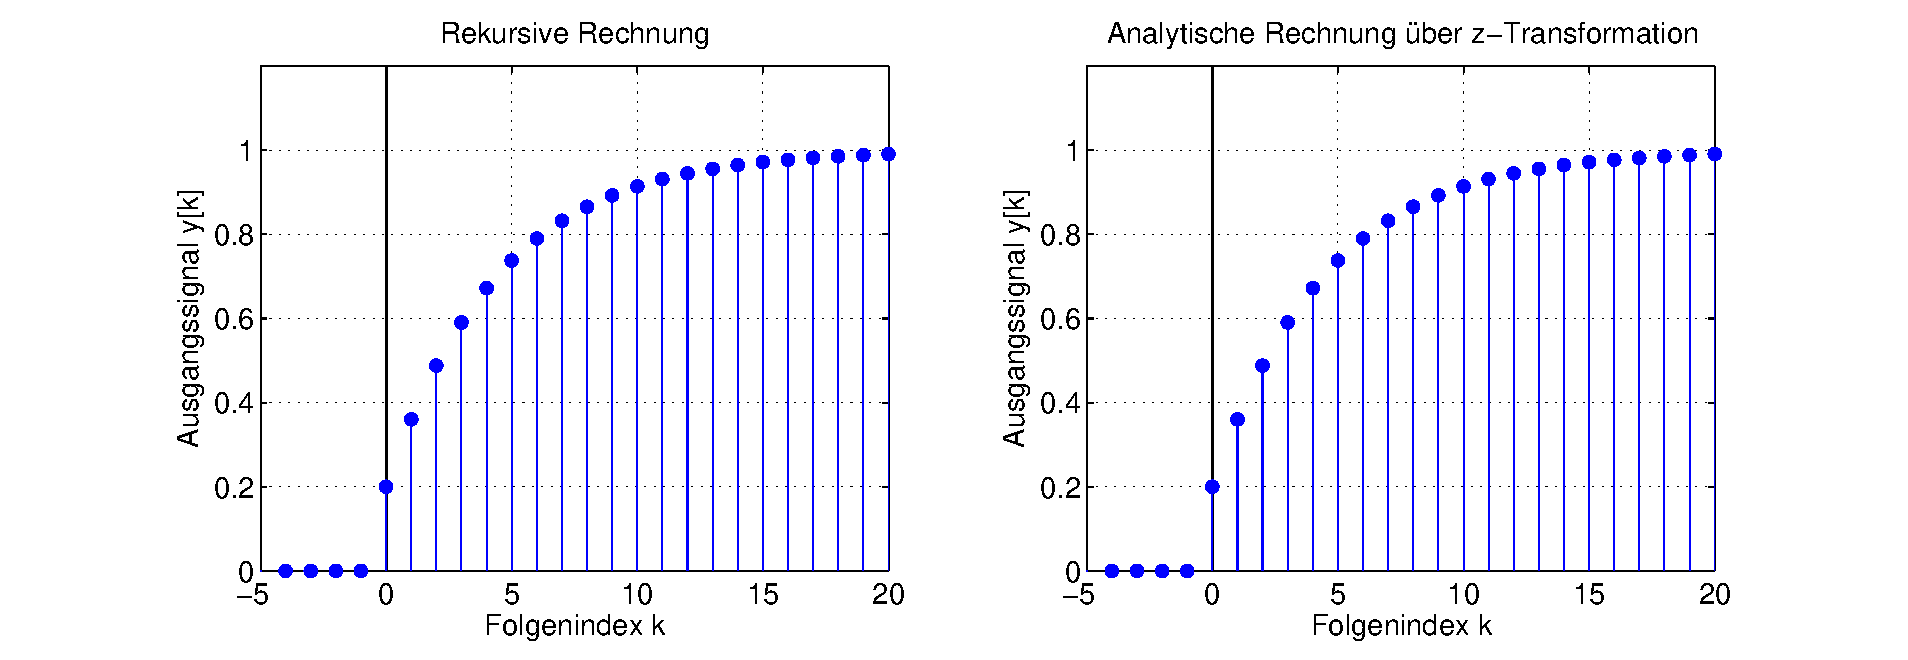
\includegraphics[width=1\textwidth]{Kapitel6/Bilder/image2.eps}}
  \caption{Ausgangssignal eines rekursiven Tiefpasses mit GF = 0.8 bei einem Eingangssprung (U${}_{0}$ = 1)}
  \label{fig:DifferenzengleichungOhneAnfangsbedingungen}
\end{figure}

\subsubsection{L\"{o}sung linearer Differenzengleichungen mit Anfangsbedingungen}

\noindent Zur L\"{o}sung linearer Differenzengleichungen mit Anfangsbedingungen wird wieder von der allgemeinen Form der Differenzengleichung ausgegangen

\begin{equation}\label{eq:sixeleven}
\sum _{n=0}^{N}c_{n} \cdot y\left[k-n\right] =\sum _{l=0}^{L}d_{l} \cdot u\left[k-l\right]
\end{equation}

\noindent Aufgrund der Zeitinvarianz kann das System um N nach links verschoben werden. Es ergibt sich die Gleichung

\begin{equation}\label{eq:sixtwelve}
\sum _{n=0}^{N}c_{n} \cdot y\left[k-n+N\right] =\sum _{l=0}^{L}d_{l} \cdot u\left[k-l+N\right]
\end{equation}

\noindent Da das Argument der Folge y[k -- n + N] damit immer gr\"{o}{\ss}er gleich k ist, muss bei der Transformation der Gleichung in den z-Bereich die Verschiebungsregel nach links angewendet werden. Im z-Bereich ergibt sich die Gleichung 

\begin{equation}\label{eq:sixthirteen}
\sum _{n=0}^{N}c_{n} \cdot \left(Y\left(z\right)\cdot z^{N-n} -z^{N-n} \cdot \sum _{k=0}^{N-n-1}y\left[k\right]\cdot z^{-k}  \right) =\sum _{l=0}^{L}d_{l} \cdot \left(U\left(z\right)\cdot z^{N-l} -z^{N-l} \cdot \sum _{k=0}^{N-l-1}u\left[k\right]\cdot z^{-k}  \right)
\end{equation}

\noindent Dieses Vorgehen \"{a}hnelt sehr der L\"{o}sung von Differentialgleichungen mit Anfangsbedingungen bei der Laplace-Transformation. In der allgemeinen Form erscheint es aufwendig. Bei praktischer Anwendung bestehen die Summen mit den Anfangswerten aber oft nur aus einzelnen Werten, sodass sich die Gleichung stark vereinfacht.\bigskip

\noindent
\colorbox{lightgray}{%
\arrayrulecolor{white}%
\renewcommand\arraystretch{0.6}%
\begin{tabular}{ wl{16.5cm} }
{\fontfamily{phv}\selectfont{Beispiel: RC-Tiefpass mit Anfangsbedingungen}}
\end{tabular}%
}\medskip

\noindent Das Vorgehen wird wieder an der Differenzengleichung eines rekursiven Tiefpasses verdeutlicht.

\begin{equation}\label{eq:sixfourteen}
y\left[k\right]-GF\cdot y\left[k-1\right]=\left(1-GF\right)\cdot u\left[k\right]
\end{equation}

\noindent Es soll die Reaktion des Tiefpasses auf einen Sprung der Eingangsgr\"{o}{\ss}e u[k] von der H\"{o}he U${}_{0}$ und f\"{u}r die Anfangsbedingungen y[0] = 2 berechnet werden. Zur Ber\"{u}cksichtigung der Anfangsbedingungen muss bei der Transformation der Gleichung in den z-Bereich die Verschiebungsregel nach links angewendet werden. Eine Index-Transformation f\"{u}hrt zu

\begin{equation}\label{eq:sixfiveteen}
y\left[k+1\right]-GF\cdot y\left[k\right]=\left(1-GF\right)\cdot u\left[k+1\right]
\end{equation}

\noindent Die Transformation in den z-Bereich ergibt

\begin{equation}\label{eq:sixsixteen}
z\cdot Y\left(z\right)-z\cdot y\left[0\right]-GF\cdot Y\left(z\right)=\left(1-GF\right)\cdot \left(z\cdot U\left(z\right)-z\cdot u\left[0\right]\right)
\end{equation}

\noindent Durch Einsetzen von U(z) und u[0] = 0 sowie Umformung

\begin{equation}\label{eq:sixseventeen}
\left(z-GF\right)\cdot Y\left(z\right)=\left(1-GF\right)\cdot \left(\frac{z^{2} }{z-1} \cdot U_{0} -z\cdot U_{0} \right)+z\cdot y\left[0\right]=\left(1-GF\right)\cdot U_{0} \cdot \left(\frac{z^{2} }{z-1} \right)+z\cdot y\left[0\right]
\end{equation}

\noindent ergibt sich die L\"{o}sung im z-Bereich

\begin{equation}\label{eq:sixeighteen}
Y\left(z\right)=\left(1-GF\right)\cdot U_{0} \cdot \left(\frac{z^{2} }{\left(z-1\right)\cdot \left(z-GF\right)} \right)+\frac{z}{z-GF} \cdot y\left[0\right]
\end{equation}

\noindent Der erste Term der z-Transformierten ist identisch zu dem Fall ohne Anfangsbedingungen in Gleichung \eqref{eq:sixeight}. Der zweite Teil beschreibt das Systemverhalten aufgrund der Anfangsbedingung und kann mit der Korrespondenztafel in den Zeitbereich zur\"{u}cktransformiert werden. Es ergibt sich das Ausgangssignal

\begin{equation}\label{eq:sixnineteen}
y\left[k\right]=\left(1-GF^{k+1} \right)\cdot U_{0} \cdot \sigma \left[k\right]+y\left[0\right]\cdot GF^{k} \cdot \sigma \left[k\right]
\end{equation}

\noindent Die Anfangsbedingung klingt \"{a}hnlich wie im zeitkontinuierlichen Bereich exponentiell ab. Bild \ref{fig:DifferenzengleichungMitAnfangsbedingungen} stellt die beiden Signalanteile dar.

\begin{figure}[H]
  \centerline{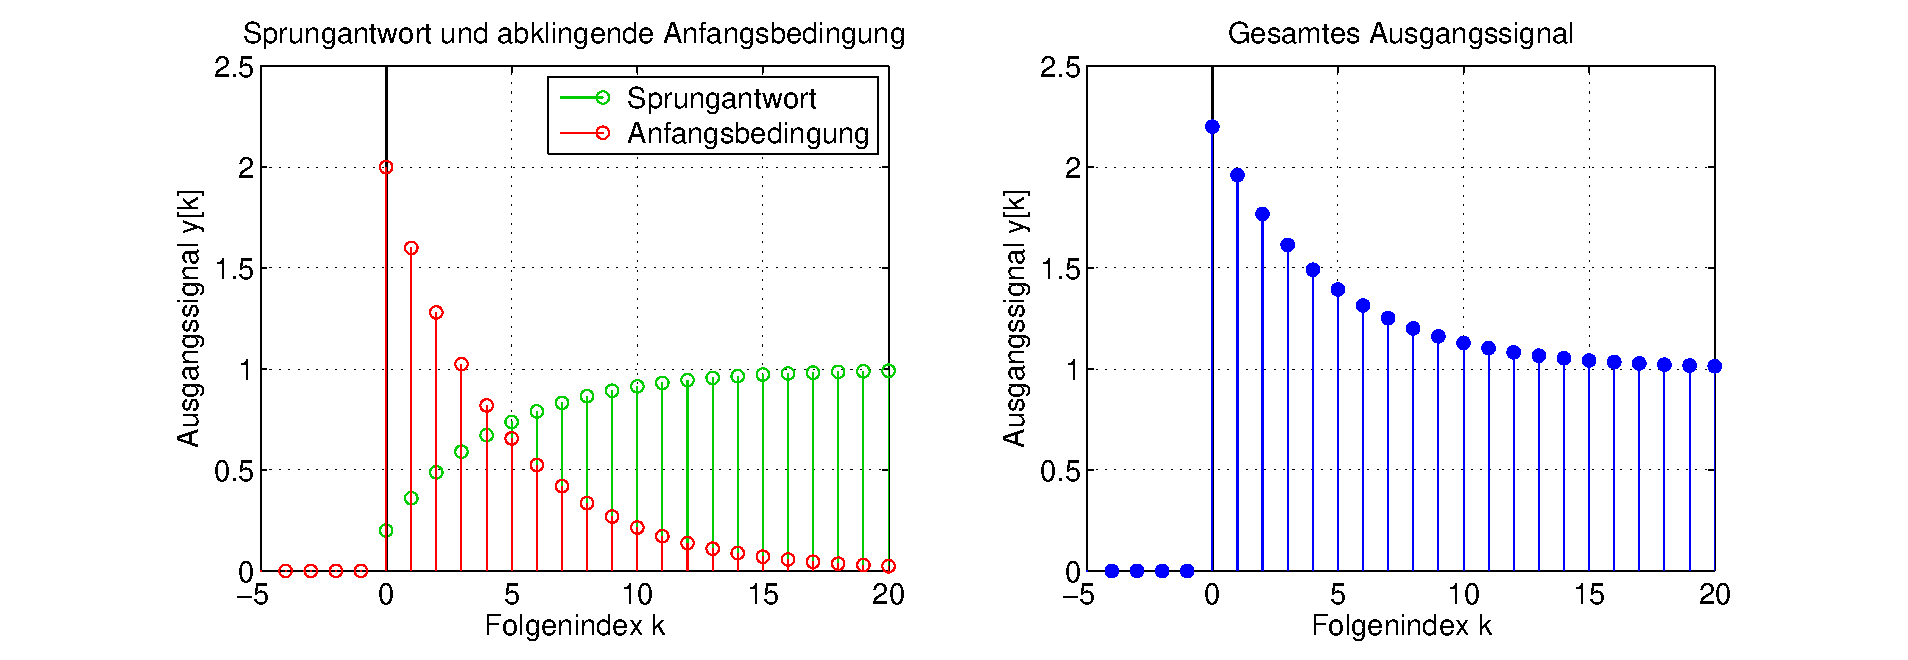
\includegraphics[width=1\textwidth]{Kapitel6/Bilder/image3.eps}}
  \caption{Ausgangssignal eines rekursiven Tiefpasses mit GF = 0.8 bei einem Eingangssprung und Anfangsbedingung y[0] = 2)}
  \label{fig:DifferenzengleichungMitAnfangsbedingungen}
\end{figure}
\clearpage
\subsubsection{Vorgehen zur L\"{o}sung linearer Differenzengleichungen}

\noindent Die beiden Abschnitte zeigen das Vorgehen zur L\"{o}sung linearer Differenzengleichungen ohne und mit Anfangsbedingungen, das in Tabelle \ref{tab:sixone} zusammengefasst ist.

\begin{table}[H]
\setlength{\arrayrulewidth}{.1em}
\caption{Vorgehen bei der Berechnung der Systemantwort mit der z-Transformation}
\setlength{\fboxsep}{0pt}%
\colorbox{lightgray}{%
\arrayrulecolor{white}%
\begin{tabular}{| wc{1.3cm} | wc{7.5cm} | wc{7.5cm} }
\hline\xrowht{20pt}

\multirow{2}{*}{\fontfamily{phv}\selectfont\textbf{Schritt}} & \multicolumn{2}{c}{\fontfamily{phv}\selectfont\textbf{Lösung einer Differenzengleichung}} \\ \xrowht{15pt}
& {\fontfamily{phv}\selectfont\textbf{ohne Anfangsbedingungen}} & 
{\fontfamily{phv}\selectfont\textbf{mit Anfangsbedingungen}} \\ \hline \xrowht{15pt}

\multirow{4}{*}{1} & \fontfamily{phv}\selectfont{Differenzengleichung}  & \fontfamily{phv}\selectfont{Verschobene Differenzengleichung} \\ \cline{2-3}\xrowht{35pt}
& $\sum _{n=0}^{N}c_{n} \cdot y\left[k-n\right] =\sum _{l=0}^{L}d_{l} \cdot u\left[k-l\right] $ & 
$\sum _{n=0}^{N}c_{n} \cdot y\left[k-n+N\right] =\sum _{l=0}^{L}d_{l} \cdot u\left[k-l+N\right] $ \\ \hline \xrowht{40pt}

2 &
\multicolumn{2}{c}{\parbox{14cm}{\centering\fontfamily{phv}\selectfont{ Transformation der Differenzengleichung in den z-Bereich unter Verwendung  der entsprechenden Verschiebungsregel}}}  \\ \hline\xrowht{20pt}

3  &
\multicolumn{2}{c}{\fontfamily{phv}\selectfont{Berechnung der z-Transformierten Y(z)}} \\ \hline\xrowht{40pt}

4  & 
\multicolumn{2}{c}{\parbox{14cm}{\centering\fontfamily{phv}\selectfont{ R\"{u}cktransformation mit Hilfe der Partialbruchzerlegung und den bekannten Korrespondenzen }}} \\ \hline 

\end{tabular}%
}
\label{tab:sixone}
\end{table}

\begin{table}[H]
\setlength{\arrayrulewidth}{.1em}
\caption{Vorgehen bei der Berechnung der Systemantwort mit der z-Transformation}
\setlength{\fboxsep}{0pt}%
\colorbox{lightgray}{%
\arrayrulecolor{white}%
\begin{tabular}{| wc{1.3cm} | wc{7.5cm} | wc{7.5cm} }
\hline\xrowht{20pt}

\multirow{2}{*}{\fontfamily{phv}\selectfont\textbf{Schritt}} & \multicolumn{2}{c}{\fontfamily{phv}\selectfont\textbf{Lösung einer Differenzengleichung}} \\ \xrowht{15pt}
& {\fontfamily{phv}\selectfont\textbf{ohne Anfangsbedingungen}} & 
{\fontfamily{phv}\selectfont\textbf{mit Anfangsbedingungen}} \\ \hline \xrowht{15pt}

\multirow{4}{*}{1} & \fontfamily{phv}\selectfont{Differenzengleichung}  & \fontfamily{phv}\selectfont{Verschobene Differenzengleichung} \\ \cline{2-3}\xrowht{35pt}
& $\sum _{n=0}^{N}c_{n} \cdot y\left[k-n\right] =\sum _{l=0}^{L}d_{l} \cdot u\left[k-l\right] $ & 
$\sum _{n=0}^{N}c_{n} \cdot y\left[k-n+N\right] =\sum _{l=0}^{L}d_{l} \cdot u\left[k-l+N\right] $ \\ \hline \xrowht{40pt}

2 &
\multicolumn{2}{c}{\parbox{14cm}{\centering\fontfamily{phv}\selectfont{ Transformation der Differenzengleichung in den z-Bereich unter Verwendung  der entsprechenden Verschiebungsregel}}}  \\ \hline\xrowht{20pt}

3  &
\multicolumn{2}{c}{\fontfamily{phv}\selectfont{Berechnung der z-Transformierten Y(z)}} \\ \hline\xrowht{40pt}

4  & 
\multicolumn{2}{c}{\parbox{14cm}{\centering\fontfamily{phv}\selectfont{ R\"{u}cktransformation mit Hilfe der Partialbruchzerlegung und den bekannten Korrespondenzen }}} \\ \hline 

\end{tabular}%
}
\label{tab:sixtwo}
\end{table}
\clearpage
\begin{table}[H]
\setlength{\arrayrulewidth}{.1em}
\caption{Beispiel f\"{u}r eine Urliste: Messwerte von 100 Widerst\"{a}nden mit einem Sollwert von $R = 1 k \Omega $}
\setlength{\fboxsep}{0pt}%
\colorbox{lightgray}{%
\arrayrulecolor{white}%
\begin{tabular}{| wc{2cm} | wc{1cm} | wc{1cm} | wc{1cm} | wc{1cm} | wc{1cm} | wc{1cm} | wc{1cm} | wc{1cm} | wc{1cm} | wc{1cm} }
\hline\xrowht{15pt}

\fontfamily{phv}\selectfont\textbf{Messung} & \multicolumn{10}{c}{\fontfamily{phv}\selectfont\textbf{Messwerte Klebermenge m / mg}} \\ \hline \xrowht{15pt}

\fontfamily{phv}\selectfont\textbf{1 - 5} &
983 & 988 & 985 & 987 & 988 & 987 & 986 & 985 & 986 & 991\\ \hline\xrowht{15pt}

\fontfamily{phv}\selectfont\textbf{6 - 10} & 
987 & 986 & 987 & 986 & 985 & 988 & 986 & 986 & 988 & 985\\ \hline\xrowht{15pt}

\fontfamily{phv}\selectfont\textbf{11- 15} &
985 & 989 & 986 & 986 & 985 & 992 & 988 & 989 & 986 & 986\\ \hline\xrowht{15pt}

\fontfamily{phv}\selectfont\textbf{16 - 20} &
985 & 986 & 986 & 986 & 989 & 988 & 986 & 986 & 986 & 987\\ \hline\xrowht{15pt}

\fontfamily{phv}\selectfont\textbf{21 - 25} &
989 & 986 & 986 & 985 & 988 & 990 & 986 & 986 & 988 & 987\\ \hline\xrowht{15pt}

\fontfamily{phv}\selectfont\textbf{26 - 30} &
985 & 989 & 987 & 985 & 986 & 990 & 986 & 985 & 986 & 988\\ \hline\xrowht{15pt}

\fontfamily{phv}\selectfont\textbf{31 - 35} &
985 & 988 & 984 & 988 & 986 & 985 & 987 & 989 & 986 & 987\\ \hline\xrowht{15pt}

\fontfamily{phv}\selectfont\textbf{36 - 40} &
987 & 987 & 985 & 987 & 986 & 986 & 986 & 987 & 985 & 989\\ \hline 

\end{tabular}%
}
\label{tab:sixthree}
\end{table}
\clearpage

\subsection{\"{U}bertragungsfunktion zeitdiskreter Systeme}

\noindent Im zeitkontinuierlichen Bereich werden Systeme durch die \"{U}bertragungsfunktion G(s) charakterisiert. Sie ergibt sich aus der Laplace-Transformierten der Differentialgleichung bei verschwindenden Anfangsbedingungen. Dasselbe Verfahren wird auch bei zeitdiskreten Systemen angewendet. Zur Berechnung der z-Transformierten Y(z) kann die Verschiebungsregel verwendet werden. Im Fall verschwindender Anfangsbedingungen ergibt sich 

\begin{equation}\label{eq:sixtwenty}
\sum _{n=0}^{N}c_{n} \cdot y\left[k-n\right] =\sum _{l=0}^{L}d_{l} \cdot u\left[k-l\right]
\end{equation}

\noindent Alternativ kann die Berechnung \"{u}ber die Faltungsregel durchgef\"{u}hrt werden. Aus der Faltung im Zeitbereich

\begin{equation}\label{eq:sixtwentyone}
y\left[k\right]=\sum _{\kappa =0}^{k}g\left[\kappa \right]\cdot u\left[k-\kappa \right] =\sum _{\kappa =0}^{k}g\left[k-\kappa \right]\cdot u\left[\kappa \right]
\end{equation}

\noindent folgt im z-Bereich 

\begin{equation}\label{eq:sixtwentytwo}
Y\left(z\right)=G\left(z\right)\cdot U\left(z\right)
\end{equation}

\noindent Durch einen Vergleich der beiden Darstellungen ergibt sich die \"{U}bertragungsfunktion f\"{u}r zeitdiskrete Systeme aus der Gleichung

\begin{equation}\label{eq:sixtwentythree}
Y\left(z\right)=G\left(z\right)\cdot U\left(z\right)=\frac{\sum _{l=0}^{L}d_{l} \cdot z^{-l}  }{\sum _{n=0}^{N}c_{n} \cdot z^{-n}  } \cdot U\left(z\right)
\end{equation}

\noindent Die \"{U}bertragungsfunktion beschreibt den Zusammenhang zwischen Ein- und Ausgangssignal im z-Bereich. 

\subsubsection{Bestimmung der Differenzengleichung aus der \"{U}bertragungsfunktion}

\noindent Wie sp\"{a}ter gezeigt wird, ist das Ergebnis eines Filterentwurfs eine \"{U}bertragungsfunktion G(z), die die definierten Filtereigenschaften besitzt. Um den Filter zum Beispiel in Form eines Mikro-Controller-Programms realisieren zu k\"{o}nnen, muss die \"{U}bertragungsfunktion 

\begin{equation}\label{eq:sixtwentyfour}
G\left(z\right)=\frac{Y\left(z\right)}{U\left(z\right)} =\frac{\sum _{l=0}^{L}d_{l} \cdot z^{-l}  }{\sum _{n=0}^{N}c_{n} \cdot z^{-n}}
\end{equation}

\noindent in eine Differenzengleichung umgeformt werden. Durch Ausmultiplizieren der beiden Br\"{u}che ergibt sich die Gleichung

\begin{equation}\label{eq:sixtwentyfive}
Y\left(z\right)\cdot \sum _{n=0}^{N}c_{n} \cdot z^{-n}  =U\left(z\right)\cdot \sum _{l=0}^{L}d_{l} \cdot z^{-l}
\end{equation}

\noindent Sie kann mit der Verschiebungsregel in den Zeitbereich zur\"{u}cktransformiert werden.

\begin{equation}\label{eq:sixtwentysix}
\sum _{n=0}^{N}c_{n} \cdot y\left[k-n\right] =\sum _{l=0}^{L}d_{l} \cdot u\left[k-l\right]
\end{equation}

\noindent Es wird deutlich, dass die Koeffizienten von Differenzengleichung und \"{U}bertragungsfunktion identisch sind. Zur Realisierung eines Filters wird der aktuelle Ausgangswert aus den vergangenen Ein- und Ausgangswerten berechnet. Dabei kann ohne Einschr\"{a}nkung der Allgemeinheit c${}_{0}$ = 1 gesetzt werden.

\begin{equation}\label{eq:sixtwentyseven}
y\left[k\right]=\sum _{l=0}^{L}d_{l} \cdot u\left[k-l\right] -\sum _{n=1}^{N}c_{n} \cdot y\left[k-n\right]
\end{equation}

\noindent Die Gleichung ist Grundlage f\"{u}r die technische Realisierung zeitdiskreter Systeme.\bigskip

\noindent
\colorbox{lightgray}{%
\arrayrulecolor{white}%
\renewcommand\arraystretch{0.6}%
\begin{tabular}{ wl{16.5cm} }
{\fontfamily{phv}\selectfont{Beispiel: Systemrealisierung}}
\end{tabular}%
}\medskip

\noindent Gegeben ist ein System mit der \"{U}bertragungsfunktion 

\begin{equation}\label{eq:sixtwentyeight}
G\left(z\right)=\frac{Y\left(z\right)}{U\left(z\right)} =\frac{0.5\cdot z}{z-0.5} =\frac{0.5}{1-0.5\cdot z^{-1} }
\end{equation}

\noindent Ausmultiplizieren

\begin{equation}\label{eq:sixtwentynine}
Y\left(z\right)\cdot \left(1-0.5\cdot z^{-1} \right)=0.5\cdot U\left(z\right)
\end{equation}

\noindent und R\"{u}cktransformation ergibt mit der Verschiebungsregel 

\begin{equation}\label{eq:sixthirty}
y\left[k\right]-0.5\cdot y\left[k-1\right]=0.5\cdot u\left[k\right]
\end{equation}

\noindent Zur Realisierung des Filters als Algorithmus muss die Gleichung nach y[k] aufgel\"{o}st werden. Das aktuelle Ausgangssignal des Filters errechnet sich damit zu

\begin{equation}\label{eq:sixthirtyone}
y\left[k\right]=\frac{1}{2} \cdot \left(u\left[k\right]+y\left[k-1\right]\right)
\end{equation}

\noindent Diese Gleichung kann zum Beispiel als Software in einem Controller oder als zeitdiskrete Schaltung realisiert werden.

\subsubsection{Impuls- und Sprungantwort}

\noindent Die \"{U}bertragungsfunktion G(z) ist die z-Transformierte der Impulsantwort. Das ergibt sich unmittelbar aus der Definitionsgleichung, wenn f\"{u}r U(z) die z-Transformierte des Impulses 

\begin{equation}\label{eq:sixthirtytwo}
U\left(z\right)=1
\end{equation}

\noindent eingesetzt wird:

\begin{equation}\label{eq:sixthirtythree}
Y\left(z\right)=G\left(z\right)\cdot U\left(z\right)=G\left(z\right)\cdot 1=G\left(z\right)
\end{equation}

\noindent Bei Anregung des Systems mit einer Sprungfolge mit der z-Transformierten

\begin{equation}\label{eq:sixthirtyfour}
U\left(z\right)=\frac{z}{z-1}
\end{equation}

\noindent ergibt sich die z-Transformierte des Ausgangssignals zu

\begin{equation}\label{eq:sixthirtyfive}
Y\left(z\right)=G\left(z\right)\cdot U\left(z\right)=G\left(z\right)\cdot \frac{z}{z-1} =H\left(z\right)
\end{equation}

\noindent Diese Gleichung kann mit der Summationsregel r\"{u}cktransformiert werden, und es ergibt sich

\begin{equation}\label{eq:sixthirtysix}
h\left[k\right]=\sum _{\kappa =0}^{k}g\left[\kappa \right]
\end{equation}

\noindent Die Sprungantwort ergibt sich aus der Summe der einzelnen Folgenwerte der Impulsantwort. Dieses Ergebnis entspricht sinngem\"{a}{\ss} den Eigenschaften zeitkontinuierlicher Systeme. Dort ist die Sprungantwort h(t) das Integral der Impulsantwort g(t). Umgekehrt kann die Impulsantwort aus der Sprungantwort berechnet werden. Im z-Bereich gilt:

\begin{equation}\label{eq:sixthirtyseven}
H\left(z\right)=\frac{z}{z-1} \cdot G\left(z\right)=\frac{1}{1-z^{-1} } \cdot G\left(z\right)
\end{equation}

\noindent Diese Gleichung kann in den Zeitbereich zur\"{u}cktransformiert werden.

\begin{equation}\label{eq:sixthirtyeight}
g\left[k\right]=h\left[k\right]-h\left[k-1\right]
\end{equation}

\noindent Auch dieses Ergebnis entspricht sinngem\"{a}{\ss} den Eigenschaften zeitkontinuierlicher Systeme. Dort ist die Impulsantwort g(t) die erweiterte Ableitung der Sprungantwort h(t). F\"{u}r zeitkontinuierliche Systeme wird der Endwert der Sprungantwort als Verst\"{a}rkung definiert. Um den Begriff der Verst\"{a}rkung f\"{u}r zeitdiskrete Systeme zu definieren, wird der Grenzwert untersucht.

\begin{equation}\label{eq:sixthirtynine}
{\mathop{\lim }\limits_{k\to \infty }} h\left[k\right]={\mathop{\lim }\limits_{z\to 1}} \left(z-1\right)\cdot H\left(z\right)=G\left(1\right)
\end{equation}

\noindent Die Verst\"{a}rkung eines zeitdiskreten Systems ergibt sich aus dem Wert der \"{U}bertragungsfunktion an der Stelle z = 1. Tabelle \ref{tab:sixtwo} fasst die Zusammenh\"{a}nge von Impuls- und Sprungantwort zusammen.

\begin{table}[H]
\setlength{\arrayrulewidth}{.1em}
\caption{\"{U}bersicht zum Zusammenhang von Impuls- und Sprungantwort}
\setlength{\fboxsep}{0pt}%
\colorbox{lightgray}{%
\arrayrulecolor{white}%
\begin{tabular}{| c | c | c |}
\hline
\parbox[c][0.3in][c]{1.9in}{\smallskip\centering\textbf{\fontfamily{phv}\selectfont{Eigenschaft}}} & 
\parbox[c][0.3in][c]{2.2in}{\smallskip\centering\textbf{\fontfamily{phv}\selectfont{Zeitbereich}}} &
\parbox[c][0.3in][c]{2.2in}{\smallskip\centering\textbf{\fontfamily{phv}\selectfont{z-Bereich}}}\\ \hline


\parbox[c][0.5in][c]{1.9in}{\centering{\fontfamily{phv}\selectfont{Impulsantwort}}} & 
\parbox[c][0.5in][c]{2.2in}{\centering{$g\left[k\right]=h\left[k\right]-h\left[k-1\right]$}} &
\parbox[c][0.5in][c]{2.2in}{\centering{$G\left(z\right)=H\left(z\right)\cdot \left(1-z^{-1} \right)$}}\\
\hline

\parbox[c][0.5in][c]{1.9in}{\centering{\fontfamily{phv}\selectfont{Sprungantwort}}} & 
\parbox[c][0.5in][c]{2.2in}{\centering{$h\left[k\right]=\sum _{\kappa =0}^{k}g\left[\kappa \right] $}} &
\parbox[c][0.5in][c]{2.2in}{\centering{$H\left(z\right)=G\left(z\right)\cdot \frac{z}{z-1} $}}\\
\hline

\parbox[c][0.5in][c]{1.9in}{\centering{\fontfamily{phv}\selectfont{Verstärkung des Systems}}} & 
\parbox[c][0.5in][c]{2.2in}{\centering{${\mathop{\lim }\limits_{k\to \infty }} \, \, h\left[k\right]$}} &
\parbox[c][0.5in][c]{2.2in}{\centering{${\mathop{\lim }\limits_{z\to 1}} \, \, \left(z-1\right)\cdot H\left(z\right)=G\left(1\right)$}}\\
\hline

\end{tabular}%
}
\label{tab:sixfour}
\end{table}

\noindent Zur Vertiefung des Begriffes der Sprungantwort werden ein zeitkontinuierliches und ein zeitdiskretes System verglichen, die an den Stellen t = k$\cdot$T${}_{A}$ dieselben Werte aufweisen.

\begin{equation}\label{eq:sixfourty}
g\left[k\right]=g\left(k\cdot T_{A} \right)
\end{equation}

\noindent Die Sprungantwort des zeitkontinuierlichen Systems ergibt sich aus dem Integral 

\begin{equation}\label{eq:sixfourtyone}
h\left(t\right)=\int _{0}^{t}g\left(\tau \right) \, \, d\tau 
\end{equation}

\noindent Die Sprungantwort des zeitdiskreten Systems ergibt sich aus der Summe

\begin{equation}\label{eq:sixfourtytwo}
h\left[k\right]=\sum _{\kappa =0}^{k}g\left[\kappa \right]
\end{equation}

\noindent W\"{a}hrend das Integral die Fl\"{a}che unter der Impulsantwort bis zum Punkt t repr\"{a}sentiert, n\"{a}hert die Summe die Fl\"{a}che \"{u}ber Rechtecke. Die Breite der Rechtecke ist bei zeitdiskreten Systemen auf den Wert eins normiert. Aus diesem Grund gilt: 

\begin{equation}\label{eq:sixfourtythree}
h\left[k\right]\ne h\left(k\cdot T_{A} \right)
\end{equation}

\noindent Die Abtastzeit kann dadurch ber\"{u}cksichtigt werden, dass die Sprungantwort h[k] mit der Abtastzeit T${}_{A}$ multipliziert wird. Damit wird die Breite der Rechtecke von 1 auf T${}_{A}$ ge\"{a}ndert. 

\begin{equation}\label{eq:sixfourtyfour}
h\left[k\right]\cdot T_{A} \approx h\left(k\cdot T_{A} \right)
\end{equation}

\noindent Auch nach dieser Korrektur sind die Sprungantworten nicht identisch, da die Fl\"{a}che unter der zeitkontinuierlichen Impulsantwort im zeitdiskreten Fall nur \"{u}ber Rechtecke approximiert wird.

\clearpage

\noindent
\colorbox{lightgray}{%
\arrayrulecolor{white}%
\renewcommand\arraystretch{0.6}%
\begin{tabular}{ wl{16.5cm} }
{\fontfamily{phv}\selectfont{Beispiel: Vergleich von Sprungantworten}}
\end{tabular}%
}\medskip

\noindent Gegeben ist ein zeitkontinuierliches System mit der Impulsantwort

\begin{equation}\label{eq:sixfourtyfive}
g\left(t\right)=2\cdot e^{-\, \frac{t}{10\, \, ms} } \cdot \sigma \left(t\right)
\end{equation}

\noindent Das System wird mit einer Abtastzeit T${}_{A}$ = 1 ms abgetastet. Es ergeben sich die Folgenwerte 

\begin{equation}\label{eq:sixfourtysix}
g\left[k\right]=2\cdot e^{-\, \frac{k}{10} } \cdot \sigma \left[k\right]
\end{equation}

\noindent Die Sprungantwort des zeitkontinuierlichen Systems lautet

\begin{equation}\label{eq:sixfourtyseven}
h\left(t\right)=\int _{0}^{t}2\cdot e^{-\, \frac{\tau }{10\, \, ms} } \, \, d\tau  =-20\, \, ms\cdot \left. e^{-\, \frac{\tau }{10\, \, ms} } \right|_{0}^{t} =20\, \, ms\cdot \left(1-e^{-\, \frac{t}{10\, \, ms} } \right)\cdot \sigma \left(t\right)
\end{equation}

\noindent Die Sprungantwort des zeitdiskreten Systems errechnet sich zu

\begin{equation}\label{eq:sixfourtyeight}
h\left[k\right]=\sum _{\kappa =0}^{k}2\cdot e^{-\, \frac{\kappa }{10} }  =2\cdot \sum _{\kappa =0}^{k}\left(e^{-\, \frac{1}{10} } \right) ^{\kappa } =2\cdot \frac{1-e^{-\, \frac{k+1}{10} } }{1-e^{-\, \frac{1}{10} } }
\end{equation}

\noindent Durch die Multiplikation der Sprungantwort mit der Abtastzeit T${}_{A}$ ergibt sich die N\"{a}herung

\begin{equation}\label{eq:sixfourtynine}
h\left(k\cdot T_{A} \right)\approx h\left[k\right]\cdot T_{A} =2\, \, ms\cdot \frac{1-e^{-\, \frac{k+1}{10} } }{1-e^{-\, \frac{1}{10}}}
\end{equation}

\noindent Die Impuls- und Sprungantworten sind in Bild \ref{fig:VergleichSprungantworten} dargestellt.

\begin{figure}[H]
  \centerline{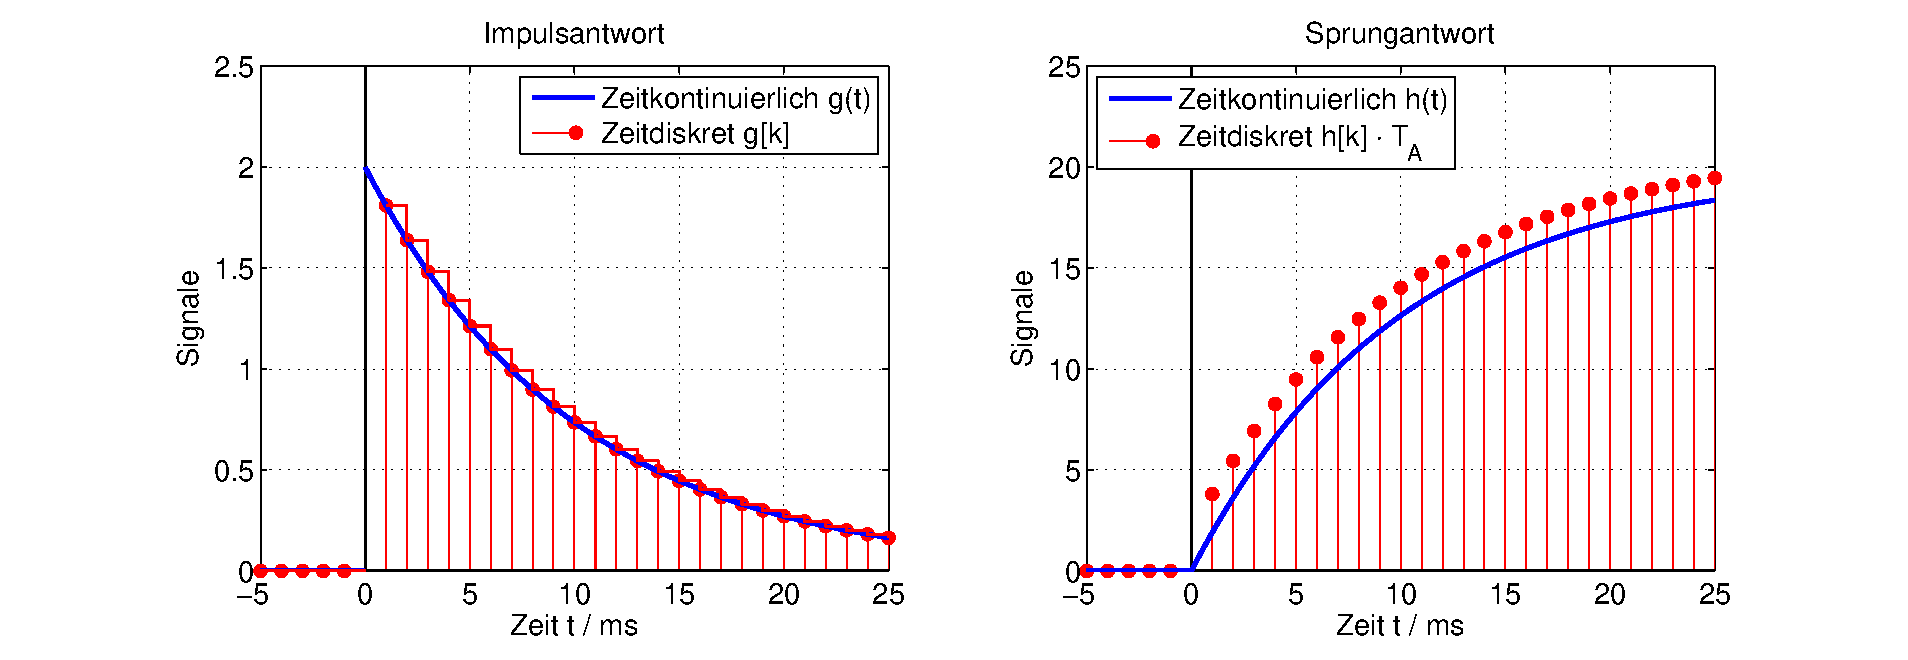
\includegraphics[width=1\textwidth]{Kapitel6/Bilder/image4.eps}}
  \caption{Vergleich der Sprungantworten eines zeitdiskreten und eines zeitkontinuierlichen Systems mit identischen Impulsantworten g[k] = g(k$\cdot$T${}_{A}$)}
  \label{fig:VergleichSprungantworten}
\end{figure}

\noindent Es wird deutlich, dass die Sprungantworten nur n\"{a}herungsweise gleich sind. Grund daf\"{u}r ist die Approximation der Fl\"{a}che unter der Impulsantwort mit den in Bild \ref{fig:VergleichSprungantworten} eingezeichneten Rechtecken. Ein ausf\"{u}hrlicher Vergleich zwischen zeitkontinuierlichen und zeitdiskreten Systemen wird in Kapitel 9 vorgenommen. 

\clearpage

\subsection{Interpretation der \"{U}bertragungsfunktion}

\noindent Gebrochen rationale \"{U}bertragungsfunktionen charakterisieren lineare, zeitinvariante Systeme im z-Bereich. An der \"{U}bertragungsfunktion lassen sich auch ohne R\"{u}cktransformation in den Zeitbereich wichtige Systemeigenschaften ablesen. In diesem Abschnitt werden wichtige Zusammenh\"{a}nge zwischen der \"{U}bertragungsfunktion im z-Bereich und dem Systemverhalten im Zeitbereich hergeleitet 

\subsubsection{Exkurs in die Darstellungsformen von \"{U}bertragungsfunktionen}

\noindent Bei der Diskussion der \"{U}bertragungsfunktion werden unterschiedliche Darstellungsformen genutzt. Sie werden an dieser Stelle miteinander verglichen und ihre Bedeutung f\"{u}r die Systemtheorie herausgearbeitet.\bigskip

{\fontfamily{phv}\selectfont
\noindent\textbf{Darstellungsformen zeitdiskreter LTI-Systeme}}\smallskip

\noindent Die Übertragungsfunktion von zeitdiskreten LTI-Systemen kann auf unterschiedliche Art darge-stellt werden. Die Beschreibung eines Systems mit der Differenzengleichung 

\begin{equation}\label{eq:sixfifty}
\sum _{n=0}^{N}c_{n} \cdot y\left[k-n\right] =\sum _{l=0}^{L}d_{l} \cdot u\left[k-l\right]
\end{equation}

\noindent ist direkt mit einer \"{U}bertragungsfunktion der Form 

\begin{equation}\label{eq:sixfiftyone}
G\left(z\right)=\frac{Y\left(z\right)}{U\left(z\right)} =\frac{\sum _{l=0}^{L}d_{l} \cdot z^{-l}  }{\sum _{n=0}^{N}c_{n} \cdot z^{-n}  }    
\end{equation}

\noindent verkn\"{u}pft. Um ein System mit Hilfe von Speichergliedern zu realisieren, wird die Gleichung nach Y(z) aufgel\"{o}st.

\begin{equation}\label{eq:sixfiftytwo}
Y\left(z\right)=\sum _{l=0}^{L}d_{l} \cdot U\left(z\right)\cdot z^{-l}  -\sum _{n=1}^{N}c_{n} \cdot Y\left(z\right)\cdot z^{-n}  =d_{0} \cdot U\left(z\right)+\sum _{n=1}^{N}\left(d_{n} \cdot U\left(z\right)-c_{n} \cdot Y\left(z\right)\right)\cdot z^{-n}   
\end{equation}

\noindent Es ergibt sich die in Bild \ref{fig:SignalflussDirektstruktur2Laplace} gezeigte kanonische Darstellungsform von Systemen mit Speichergliedern.

\begin{figure}[H]
  \centerline{\includegraphics[width=0.5\textwidth]{Kapitel6/Bilder/image5.png}}
  \caption{Kanonisches Blockschaltbild eines linearen, zeitinvarianten Systems im zeitkontinuierlichen Bereich}
  \label{fig:SignalflussDirektstruktur2Laplace}
\end{figure}

\noindent Durch Erweiterung der \"{U}bertragungsfunktion \eqref{eq:sixfiftyone} mit z${}^{N}$ ergibt sich eine \"{U}bertragungsfunktion, bei der f\"{u}r d${}_{0}$ $\neq$ 0 Z\"{a}hler- und Nennergrad identisch sind.

\begin{equation}\label{eq:sixfiftythree}
G\left(z\right)=\frac{Y\left(z\right)}{U\left(z\right)} =\frac{z^{N} \cdot \sum _{l=0}^{L}d_{l} \cdot z^{-l}  }{z^{N} \cdot \sum _{n=0}^{N}c_{n} \cdot z^{-n}  } =\frac{\sum _{m=0}^{M}b_{m} \cdot z^{m}  }{\sum _{n=0}^{N}a_{n} \cdot z^{n}  } 
\end{equation}

\noindent Diese Darstellungsform wird bei der R\"{u}cktransformation einer z-Transformierten G(z) durch Partialbruchzerlegung eingesetzt. \bigskip

\noindent
\colorbox{lightgray}{%
\arrayrulecolor{white}%
\renewcommand\arraystretch{0.6}%
\begin{tabular}{ wl{16.5cm} }
{\fontfamily{phv}\selectfont{Beispiel: Darstellungsformen von \"{U}bertragungsfunktionen}}
\end{tabular}%
}\medskip

\noindent Gegeben ist ein System mit der Differenzengleichung

\begin{equation}\label{eq:sixfiftyfour}
y\left[k\right]+3\cdot y\left[k-1\right]+2\cdot y\left[k-2\right]=u\left[k\right]+4\cdot u\left[k-1\right] 
\end{equation}

\noindent und der daraus resultierenden \"{U}bertragungsfunktion 

\begin{equation}\label{eq:sixfiftyfive}
G\left(z\right)=\frac{Y\left(z\right)}{U\left(z\right)} =\frac{1+4\cdot z^{-1} }{1+3\cdot z^{-1} +2\cdot z^{-2} } 
\end{equation}

\noindent Aufl\"{o}sen nach Y(z) ergibt

\begin{equation}\label{eq:sixfiftysix}
Y\left(z\right)=U\left(z\right)+\left(4\cdot U\left(z\right)-3\cdot Y\left(z\right)-2\cdot Y\left(z\right)\cdot z^{-1} \right)\cdot z^{-1}
\end{equation}

\noindent Bild \ref{fig:SignalflussDirektstruktur2zBereichBeispiel} zeigt die kanonische Darstellungsform des Systems mit Speichergliedern.

\begin{figure}[H]
  \centerline{\includegraphics[width=0.5\textwidth]{Kapitel6/Bilder/image6.png}}
  \caption{Kanonisches Blockschaltbild Systems mit der Differenzengleichung \eqref{eq:sixfiftyfour}}
  \label{fig:SignalflussDirektstruktur2zBereichBeispiel}
\end{figure}

\noindent Die \"{U}bertragungsfunktion hat im Z\"{a}hler eine Ordnung von M = 1 und im Nenner eine Ordnung N = 2. Erweitern der \"{U}bertragungsfunktion mit z² f\"{u}hrt zu der Darstellung

\begin{equation}\label{eq:sixfiftyseven}
G\left(z\right)=\frac{z^{2} +4\cdot z}{z^{2} +3\cdot z+2}
\end{equation}

\noindent Z\"{a}hler- und Nennerpolynom haben denselben Grad N = 2. Nach Polynomdivision ergibt sich eine echt gebrochen rationale Funktion

\begin{equation}\label{eq:sixfiftyeight}
G\left(z\right)=\frac{z^{2} +4\cdot z}{z^{2} +3\cdot z+2} =1+\frac{z-2}{z^{2} +3\cdot z+2}
\end{equation}

\noindent Sie kann als Summe von Partialbr\"{u}chen dargestellt 

\begin{equation}\label{eq:sixfiftynine}
G\left(z\right)=1+\frac{z-2}{z^{2} +3\cdot z+2} =1-\frac{3}{z+1} +\frac{4}{z+2} =1-3\cdot \frac{z}{z+1} \cdot z^{-1} +4\cdot \frac{z}{z+2} \cdot z^{-1}
\end{equation}

\noindent und in den Zeitbereich zur\"{u}cktransformiert werden.

\begin{equation}\label{eq:sixsixty}
g\left[k\right]=\delta \left[k\right]-3\cdot \left(-1\right)^{k-1} \cdot \sigma \left[k-1\right]+4\cdot \left(-2\right)^{k-1} \cdot \sigma \left[k-1\right]
\end{equation}

\clearpage

{\fontfamily{phv}\selectfont
\noindent\textbf{Darstellungsformen zeitkontinuierlicher LTI-Systeme}}\smallskip

\noindent Auch bei zeitkontinuierlichen Systemen kann die \"{U}bertragungsfunktion auf unterschiedliche Arten dargestellt werden. In Teil A dieser Buchreihe wird in Kapitel 5 ausgehend von einer Differentialgleichung N-ter Ordnung

\begin{equation}\label{eq:sixsixtyone}
\sum _{n=0}^{N}a_{n} \cdot \frac{d^{n} y}{dt^{n} }  =\sum _{m=0}^{M}b_{m} \cdot \frac{d^{m} u}{dt^{m} } 
\end{equation}

\noindent die \"{U}bertragungsfunktion 

\begin{equation}\label{eq:sixsixtytwo}
G\left(s\right)=\frac{Y\left(s\right)}{U\left(s\right)} =\frac{\sum _{m=0}^{M}b_{m} \cdot s^{m}  }{\sum _{n=0}^{N}a_{n} \cdot s^{n}  }
\end{equation}

\noindent bestimmt. Die Interpretation des Systems erfolgt anhand dieser Darstellungsform mit Z\"{a}hler- und Nennerpolynom. Da die Differentiation im Zeitbereich nicht kausal ist, kann diese Darstellungsform jedoch nicht zur Simulation zeitkontinuierlicher LTI-Systeme verwendet werden. Deshalb wird im Abschnitt 3.5 von Teil A dieser Buchreihe die Differentialgleichung N-mal integriert. Analog zu Gleichung \eqref{eq:sixfiftyone} ergibt sich der Ausdruck

\begin{equation}\label{eq:sixsixtythree}
G\left(s\right)=\frac{Y\left(s\right)}{U\left(s\right)} =\frac{\sum _{m=0}^{M}b_{m} \cdot s^{m}  }{\sum _{n=0}^{N}a_{n} \cdot s^{n}  } =\frac{\frac{1}{s^{N} } \cdot \sum _{m=0}^{M}b_{m} \cdot s^{m}  }{\frac{1}{s^{N} } \cdot \sum _{n=0}^{N}a_{n} \cdot s^{n}  } =\frac{\sum _{m=0}^{M}b_{m} \cdot s^{m-N}  }{\sum _{n=0}^{N}a_{n} \cdot s^{n-N}  } =\frac{\sum _{l=0}^{N}d_{l} \cdot s^{-l}  }{\sum _{n=0}^{N}c_{n} \cdot s^{-n}  }
\end{equation}

\noindent Ausmultiplizieren der Gleichung 

\begin{equation}\label{eq:sixsixtyfour}
Y\left(s\right)\cdot \sum _{n=0}^{N}c_{n} \cdot s^{-n}  =U\left(s\right)\cdot \sum _{l=0}^{N}d_{l} \cdot s^{-l}
\end{equation}

\noindent und Aufl\"{o}sen nach Y(s) f\"{u}hrt mit c${}_{0}$ = 1 zu dem Ausdruck

\begin{equation}\label{eq:sixsixtyfive}
\begin{split}
Y\left(s\right) &=U\left(s\right)\cdot \sum _{l=0}^{N}d_{l} \cdot s^{-l}  -Y\left(s\right)\cdot \sum _{n=1}^{N}c_{n} \cdot s^{-n}\\
&=\sum _{l=0}^{N}d_{l}\cdot U(s)\cdot s^{-l}-\sum _{n=1}^{N}c_{n}c_{n}\cdot Y(s) \cdot s^{-n}
\end{split}
\end{equation}

\noindent Um die Integrierer zusammenfassen zu k\"{o}nnen, wird die erste Summe zerlegt.

\begin{equation}\label{eq:sixsixtysix}
Y\left(s\right)=\sum _{l=0}^{N}d_{l} \cdot U\left(s\right)\cdot s^{-l}  -\sum _{n=1}^{N}c_{n} \cdot Y\left(s\right)\cdot s^{-n}  =d_{0} \cdot U\left(s\right)+\sum _{l=1}^{N}d_{l} \cdot U\left(s\right)\cdot s^{-l}  -\sum _{n=1}^{N}c_{n} \cdot Y\left(s\right)\cdot s^{-n}
\end{equation}

\noindent Damit k\"{o}nnen die beiden \"{u}brigen Summen zusammengefasst werden.

\begin{equation}\label{eq:sixsixtyseven}
Y\left(s\right)=d_{0} \cdot U\left(s\right)+\sum _{n=1}^{N}\left(d_{l} \cdot U\left(s\right)-c_{n} \cdot Y\left(s\right)\right)\cdot s^{-n}
\end{equation}
\clearpage
\noindent Es ergibt sich die in Bild \ref{fig:AGAIN} gezeigte kanonische Darstellungsform von Systemen mit Integrierern.

\begin{figure}[H]
  \centerline{\includegraphics[width=0.5\textwidth]{Kapitel6/Bilder/image5.png}}
  \caption{Kanonisches Blockschaltbild eines linearen, zeitinvarianten Systems im zeitkontinuierlichen Bereich}
  \label{fig:AGAIN}
\end{figure} \bigskip

\noindent
\colorbox{lightgray}{%
\arrayrulecolor{white}%
\renewcommand\arraystretch{0.6}%
\begin{tabular}{ wl{16.5cm} }
{\fontfamily{phv}\selectfont{Beispiel: Darstellungsformen der \"{U}bertragungsfunktion f\"{u}r ein Feder-Masse-D\"{a}mpfer-Systems}}
\end{tabular}%
}\medskip

\noindent Die unterschiedlichen Darstellungsformen f\"{u}r zeitkontinuierliche Systeme werden anhand eines Feder-Masse-D\"{a}mpfer-Systems mit der Differentialgleichung 

\begin{equation}\label{eq:sixsixtyeight}
F_{E} \left(t\right)=m\cdot \frac{d^{2} x}{dt^{2} } +D\cdot \frac{dx}{dt} +c\cdot x\left(t\right)
\end{equation}

\noindent verdeutlicht. Eingangssignal ist der Kraftverlauf F${}_{E}$(t), Ausgangssignal ist die Auslenkung x(t). Transformation in den Laplace-Bereich ergibt bei verschwindenden Anfangsbedingungen die Gleichung

\begin{equation}\label{eq:sixsixtynine}
F_{E} \left(s\right)=m\cdot s^{2} \cdot X\left(s\right)+D\cdot s\cdot X\left(s\right)+c\cdot X\left(s\right)
\end{equation}

\noindent Damit lautet die \"{U}bertragungsfunktion

\begin{equation}\label{eq:sixseventy}
\frac{X\left(s\right)}{F_{E} \left(s\right)} =\frac{1}{m\cdot s^{2} +D\cdot s+c} =\frac{1}{m} \cdot \frac{1}{s^{2} +\frac{D}{m} \cdot s+\frac{c}{m} }
\end{equation}

\noindent Auf Basis dieser Darstellung und den Polen des Systems

\begin{equation}\label{eq:sixseventyone}
\alpha _{1,2} =-\frac{D}{2\cdot m} \pm \sqrt{\frac{D^{2} }{4\cdot m^{2} } -\frac{c}{m} }
\end{equation}

\noindent k\"{o}nnen die Systemeigenschaften diskutiert werden. Andererseits erfolgt die Systemsimulation \"{u}ber eine Darstellungsform

\begin{equation}\label{eq:sixseventytwo}
\frac{X\left(s\right)}{F_{E} \left(s\right)} =\frac{\frac{1}{s^{2} } }{m+\frac{D}{s} +\frac{c}{s^{2} } }
\end{equation}

\noindent Sie kann nach X(s) aufgel\"{o}st werden

\begin{equation}\label{eq:sixseventythree}
X\left(s\right)=\frac{1}{m} \cdot \left(\frac{1}{s^{2} } \cdot F_{E} \left(s\right)-\frac{D}{s} \cdot X\left(s\right)-\frac{c}{s^{2} } \cdot X\left(s\right)\right)
\end{equation}

Es ergibt sich das in Bild \ref{fig:FederMasseDaempferDirektstruktur2} dargestellte kanonische Blockschaltbild. 

\begin{figure}[H]
  \centerline{\includegraphics[width=0.5\textwidth]{Kapitel6/Bilder/image8.png}}
  \caption{Kanonisches Blockschaltbild eines Feder-Masse-D\"{a}mpfer-Systems}
  \label{fig:FederMasseDaempferDirektstruktur2}
\end{figure}

\noindent Je nach Anwendungsfall wird die Darstellung mit Z\"{a}hler- und Nennerpolynom oder die Darstellung \"{u}ber Integrierglieder mit der Laplace-Transformierten 1/s verwendet.\bigskip

{\fontfamily{phv}\selectfont
\noindent\textbf{Zusammenfassung der Darstellungsformen von Übertragungsfunktionen}}\smallskip

\noindent \"{U}bertragungsfunktionen werden damit sowohl bei zeitkontinuierlichen als auch bei zeitdiskreten Systemen in zwei Darstellungsformen behandelt. Sie sind in Tabelle \ref{tab:sixthree} zusammen mit ihrer Anwendung dargestellt.

\begin{table}[H]
\setlength{\arrayrulewidth}{.1em}
\caption{\"{U}bersicht zu Darstellungsformen von \"{U}bertragungsfunktionen und ihrer Anwendung}
\setlength{\fboxsep}{0pt}%
\colorbox{lightgray}{%
\arrayrulecolor{white}%
\begin{tabular}{| c | c | c |}
\hline
\parbox[c][0.3in][c]{1.9in}{\smallskip\centering\textbf{\fontfamily{phv}\selectfont{Anwendung}}} & 
\parbox[c][0.3in][c]{2.2in}{\smallskip\centering\textbf{\fontfamily{phv}\selectfont{Zeitkontinuierliche Systeme}}} &
\parbox[c][0.3in][c]{2.2in}{\smallskip\centering\textbf{\fontfamily{phv}\selectfont{Zeitdiskrete Systeme}}}\\ \hline


\parbox[c][1in][c]{1.9in}{\centering{\fontfamily{phv}\selectfont{Mathematische Diskussion der \"{U}bertragungsfunktion}}} & 
\parbox[c][1in][c]{2.2in}{\centering{$G\left(s\right)=\frac{\sum _{m=0}^{M}b_{m} \cdot s^{m}  }{\sum _{n=0}^{N}a_{n} \cdot s^{n}  } $}} &
\parbox[c][1in][c]{2.2in}{\centering{$G\left(z\right)=\frac{\sum _{m=0}^{M}b_{m} \cdot z^{m}  }{\sum _{n=0}^{N}a_{n} \cdot z^{n}  } $}}\\
\hline

\parbox[c][1in][c]{1.9in}{\centering{\fontfamily{phv}\selectfont{Darstellungsform zur Realisierung der Systeme}}} & 
\parbox[c][1in][c]{2.2in}{\centering{$G\left(s\right)=\frac{\sum _{l=0}^{L}d_{l} \cdot s^{-l}  }{\sum _{n=0}^{N}c_{n} \cdot s^{-n}  } $}} &
\parbox[c][1in][c]{2.2in}{\centering{$G\left(z\right)=\frac{\sum _{l=0}^{L}d_{l} \cdot z^{-l}  }{\sum _{n=0}^{N}c_{n} \cdot z^{-n}  } $}}\\
\hline


\end{tabular}%
}
\label{tab:sixfive}
\end{table}

\noindent Die folgende Diskussion der \"{U}bertragungsfunktion zeitdiskreter Systeme bezieht sich damit auf eine \"{U}bertragungsfunktion der Form

\begin{equation}\label{eq:sixseventyfour}
G\left(z\right)=\frac{\sum _{m=0}^{M}b_{m}\cdot z^{m}}{\sum _{n=0}^{N}a_{n} \cdot z^{n}}
\end{equation}

\subsubsection{Pol-Nullstellen-Diagramme}

\noindent Die Interpretation der \"{U}bertragungsfunktion erlaubt Aussagen \"{u}ber Stabilit\"{a}t, Schwingungsneigung und Sprungf\"{a}higkeit von Systemen. Ein wesentlicher Schritt zur Interpretation des Systems ist die Analyse der unterschiedlichen Pole $\alpha_{n}$ und der unterschiedlichen Nullstellen $\beta_{m}$. Dazu wird die \"{U}bertragungsfunktion durch Linearfaktoren dargestellt. 

\begin{equation}\label{eq:sixseventyfive}
G\left(z\right)=\frac{B\left(z\right)}{A\left(z\right)} =\frac{\sum _{m=0}^{M}b_{m} \cdot z^{m}  }{\sum _{n=0}^{N}a_{n} \cdot z^{n}  } =\frac{b_{M} }{a_{N} } \cdot \frac{\left(z-\beta _{1} \right)^{M_{1} } \cdot \left(z-\beta _{2} \right)^{M_{2} } \cdot ...}{\left(z-\alpha _{1} \right)^{N_{1} } \cdot \left(z-\alpha _{2} \right)^{N_{2} } \cdot ...}
\end{equation}

\noindent Die Pole $\alpha_{n}$ und Nullstellen $\beta_{m}$ k\"{o}nnen zur besseren \"{U}bersicht in der komplexen Ebene dargestellt werden. Dabei werden Nullstellen mit einem Kreis und Pole mit einem Kreuz dargestellt, ihre Vielfachheit N${}_{n}$ und M${}_{m}$ wird in Klammern angegeben. Die Diagramme werden als Pol-Nullstellen-Diagramme oder als Pole-Zero-Maps bezeichnet.\bigskip

\noindent
\colorbox{lightgray}{%
\arrayrulecolor{white}%
\renewcommand\arraystretch{0.6}%
\begin{tabular}{ wl{16.5cm} }
{\fontfamily{phv}\selectfont{Beispiel: Pol-Nullstellen-Diagramm}}
\end{tabular}%
}\medskip

\noindent Ein System mit der Differenzengleichung 

\begin{equation}\label{eq:sixseventysix}
y\left[k\right]-0.2\cdot y\left[k-1\right]+0.15\cdot y\left[k-2\right]=u\left[k\right]+1.5\cdot u\left[k-1\right]
\end{equation}

\noindent weist eine \"{U}bertragungsfunktion 

\begin{equation}\label{eq:sixseventyseven}
G\left(z\right)=\frac{Y\left(z\right)}{U\left(z\right)} =\frac{1+1.5\cdot z^{-1} }{1-0.2\cdot z^{-1} +0.15\cdot z^{-2} } =\frac{z^{2} +1.5\cdot z}{z^{2} -0.2\cdot z+0.15} =\frac{z\cdot \left(z+1.5\right)}{\left(z-0.5\right)\cdot \left(z+0.3\right)}
\end{equation}

\noindent auf. Sie besitzt die Nullstellen $\beta_{1}$ = - 1.5 und $\beta_{2}$ = 0, sowie die reellen Polstellen $\alpha_{1}$ = - 0.3 und $\alpha_{2}$ = 0.5. Es ergibt sich das in Bild \ref{fig:zSysteme_PolNullstellenDiagramm} dargestellte Pol-Nullstellen-Diagramm.

\begin{figure}[H]
  \centerline{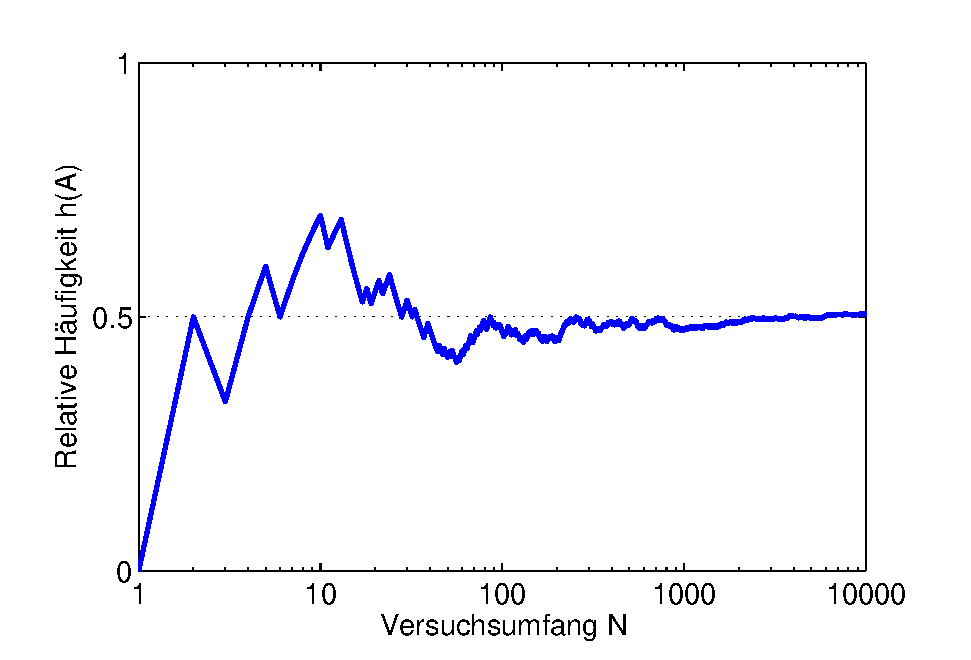
\includegraphics[width=0.5\textwidth]{Kapitel6/Bilder/image9.eps}}
  \caption{Pol-Nullstellen-Diagramm des Systems aus Gleichung \eqref{eq:sixseventyfive}}
  \label{fig:zSysteme_PolNullstellenDiagramm}
\end{figure}

\noindent Das Pol-Nullstellen-Diagramm bietet einen guten \"{U}berblick \"{u}ber die Lage der Pole und Nullstellen in der komplexen Ebene.

\subsubsection{\"{U}bertragungsfunktion und Kausalit\"{a}t von Systemen}

\noindent Zur \"{U}berpr\"{u}fung der Kausalit\"{a}t eines Systems mit der \"{U}bertragungsfunktion 

\begin{equation}\label{eq:sixseventeight}
G\left(z\right)=\frac{Y\left(z\right)}{U\left(z\right)} =\frac{\sum _{m=0}^{M}b_{m} \cdot z^{m}  }{\sum _{n=0}^{N}a_{n} \cdot z^{n}  } =\frac{\sum _{m=0}^{M}b_{m} \cdot z^{m-N}  }{\sum _{n=0}^{N}a_{n} \cdot z^{n-N}  }
\end{equation}

\noindent werden Z\"{a}hler- und Nennerpolynom durch z${}^{N}$ dividiert. Ausmultiplizieren und Aufl\"{o}sen der Summen f\"{u}hrt zur Gleichung 

\begin{equation}\label{eq:sixseventnine}
Y\left(z\right)\cdot \left(a_{N} +...+a_{0} \cdot z^{-N} \right)=U\left(z\right)\cdot \left(b_{M} \cdot z^{M-N} +...+b_{0} \cdot z^{-N} \right)
\end{equation}

\noindent R\"{u}cktransformation ergibt f\"{u}r verschwindende Anfangsbedingungen 

\begin{equation}\label{eq:sixseighty}
a_{N} \cdot y\left[k\right]+...+a_{0} \cdot y\left[k-N\right]=b_{M} \cdot u\left[k+M-N\right]+...+b_{0} \cdot u\left[k-N\right]
\end{equation}

\noindent Das System ist kausal, wenn y[k] nur von aktuellen und vergangenen Eingangswerten abh\"{a}ngt. Das ist der Fall, wenn die Bedingung M $\leq$ N erf\"{u}llt ist. Der Z\"{a}hlergrad der \"{U}bertragungsfunktion darf maximal so gro{\ss} sein wie der Nennergrad, damit das System kausal ist.\bigskip

\noindent
\colorbox{lightgray}{%
\arrayrulecolor{white}%
\renewcommand\arraystretch{0.6}%
\begin{tabular}{ wl{16.5cm} }
{\fontfamily{phv}\selectfont{Beispiel: Nicht kausales System}}
\end{tabular}%
}\medskip

\noindent Gegeben ist ein System mit der \"{U}bertragungsfunktion

\begin{equation}\label{eq:sixseightyone}
G\left(z\right)=\frac{Y\left(z\right)}{U\left(z\right)} =\frac{3\cdot z^{2} +z+2}{2\cdot z+1}
\end{equation}

\noindent Der Z\"{a}hlergrad M = 2 ist gr\"{o}{\ss}er als der Nennergrad N = 1. Das System ist demnach nicht kausal. Umformen der \"{U}bertragungsfunktion f\"{u}hrt zu

\begin{equation}\label{eq:sixseightytwo}
Y\left(z\right)\cdot \left(2\cdot z+1\right)=U\left(z\right)\cdot \left(3\cdot z^{2} +z+2\right)
\end{equation}

\noindent beziehungsweise

\begin{equation}\label{eq:sixseightythree}
Y\left(z\right)\cdot \left(2+z^{-1} \right)=U\left(z\right)\cdot \left(3\cdot z+1+2\cdot z^{-1} \right)
\end{equation}

\noindent R\"{u}cktransformation f\"{u}hrt bei verschwindenden Anfangsbedingungen zu der Differenzengleichung

\begin{equation}\label{eq:sixseightyfour}
2\cdot y\left[k\right]+y\left[k-1\right]=3\cdot u\left[k+1\right]+u\left[k\right]+2\cdot u\left[k-1\right]
\end{equation}

\noindent Der aktuelle Ausgangswert

\begin{equation}\label{eq:sixseightyfive}
y\left[k\right]=\frac{1}{2} \cdot \left(3\cdot u\left[k+1\right]+u\left[k\right]+2\cdot u\left[k-1\right]-y\left[k-1\right]\right)
\end{equation}

\noindent ist von dem zuk\"{u}nftigen Wert u[k+1] abh\"{a}ngig, das System ist damit nicht kausal.

\subsubsection{\"{U}bertragungsfunktion mit Z\"{a}hlergrad M gleich Nennergrad N}

\noindent F\"{u}r kausale Systeme ist der Z\"{a}hlergrad M der \"{U}bertragungsfunktion kleiner oder gleich dem Nennergrad N. F\"{u}r den Fall M = N muss vor der Partialbruchzerlegung eine Polynomdivision durchgef\"{u}hrt werden. Dadurch entsteht im Ausdruck f\"{u}r die \"{U}bertragungsfunktion G(z) ein konstanter Summand. Da die inverse z-Transformierte zu einer Konstanten die Impulsfolge $\delta$[k] ist, entspricht diesem Summand im Zeitbereich der Folgenwert f\"{u}r k = 0

\begin{equation}\label{eq:sixseightysix}
g\left[k=0\right]=\frac{b_{M} }{a_{N}}
\end{equation}

\noindent Alle weiteren Summanden der Partialbruchzerlegung werden im Zeitbereich mit Sprungfunktionen der Form $\sigma$[k - 1] multipliziert und sind erst f\"{u}r k $\mathrm{>}$ 0 von null verschieden. Damit ist ein System nur dann sprungf\"{a}hig, wenn der Z\"{a}hlergrad M gleich dem Nennergrad N ist. \bigskip

\noindent
\colorbox{lightgray}{%
\arrayrulecolor{white}%
\renewcommand\arraystretch{0.6}%
\begin{tabular}{ wl{16.5cm} }
{\fontfamily{phv}\selectfont{Beispiel: Sprungf\"{a}higes System}}
\end{tabular}%
}\medskip

\noindent Die \"{U}bertragungsfunktion G(z) soll interpretiert werden. Da der Z\"{a}hlergrad genauso gro{\ss} ist wie der Nennergrad, wird eine Polynomdivision durchgef\"{u}hrt. Um auf einen Ausdruck der Korrespondenztafel zu kommen, muss der Restbruch mit z erweitert werden.

\begin{equation}\label{eq:sixseightyseven}
G\left(z\right)=\frac{2+z^{-1} }{1-0.2\cdot z^{-1} } =\frac{2\cdot z+1}{z-0.2} =2+\frac{1.4}{z-0.2} =2+\frac{1.4\cdot z}{z-0.2} \cdot z^{-1}
\end{equation}

\noindent Damit kann die Impulsantwort mit der Korrespondenztafel und der Verschiebungsregel bestimmt werden zu

\begin{equation}\label{eq:sixseightyeight}
g\left[k\right]=2\cdot \delta \left[k\right]+1.4\cdot 0.2^{k-1} \cdot \sigma \left[k-1\right]
\end{equation}

\noindent Sie springt an der Stelle k = 0 auf den Wert 2.

\subsubsection{Partialbruchzerlegung mit einfachen reellen Polen}

\noindent Besitzt die \"{U}bertragungsfunktion einfache reelle Pole $\alpha_{n}$ $\neq$ 0, kann sie \"{u}ber die Partialbruchzerlegung dargestellt werden als

\begin{equation}\label{eq:sixseightynine}
G\left(z\right)=\sum _{n=1}^{N}\frac{A_{n} }{z-\alpha _{n}}
\end{equation}

\noindent Jeder einzelne Partialbruch hat die Form 

\begin{equation}\label{eq:sixsninety}
G_{n} \left(z\right)=\frac{A_{n} }{z-\alpha _{n} } =A_{n} \cdot \frac{z}{z-\alpha _{n} } \cdot z^{-1}
\end{equation}

\noindent Im Zeitbereich ergibt sich damit f\"{u}r jeden Partialbruch eine Exponentialfunktion, die um einen Folgenindex nach rechts verschoben ist:

\begin{equation}\label{eq:sixsninetyone}
g_{n} \left[k\right]=A_{n} \cdot \alpha _{n}^{k-1} \cdot \sigma \left[k-1\right]
\end{equation}

\noindent Die Summe der einzelnen Partialbr\"{u}che entspricht deshalb im Zeitbereich der Folge

\begin{equation}\label{eq:sixsninetytwo}
g\left[k\right]=\sum _{n=1}^{N}A_{n} \cdot \alpha _{n}^{k-1} \cdot \sigma \left[k-1\right]
\end{equation}

\noindent Der Betrag der Pole $\alpha_{n}$ entscheidet \"{u}ber die Frage, ob die Impulsantwort konvergent oder divergent ist und damit \"{u}ber die Stabilit\"{a}t des Systems. 

\noindent Die Impulsantwort beginnt bei sprungf\"{a}higen Systemen bei k = 0 und bei nicht sprungf\"{a}higen Systemen bei k = 1, und sie ist unendlich lang. Deshalb werden wird die Impulsantwort als Infinite-Impulse-Response und die Systeme als Infinite-Impulse-Response-Systeme (IIR-Systeme) bezeichnet. IIR-Systeme sind daran zu erkennen, dass zumindest ein Pol $\alpha_{n}$ der \"{U}bertragungsfunktion nicht im Koordinatenursprung liegt.\bigskip

\noindent
\colorbox{lightgray}{%
\arrayrulecolor{white}%
\renewcommand\arraystretch{0.6}%
\begin{tabular}{ wl{16.5cm} }
{\fontfamily{phv}\selectfont{Beispiel: \"{U}bertragungsfunktion mit einfachen reellen Polen}}
\end{tabular}%
}\medskip

\noindent Die untenstehende \"{U}bertragungsfunktion G(z) soll interpretiert werden. Ihr Z\"{a}hlergrad ist kleiner als der Nennergrad, und sie hat zwei einfache reelle Pole. Die \"{U}bertragungsfunktion kann in Partialbr\"{u}che zerlegt werden.

\begin{equation}\label{eq:sixsninetythree}
\begin{split}
G\left(z\right)&=\frac{3\cdot z^{-1} -3.5\cdot z^{-2} }{1-2\cdot z^{-1} +0.75\cdot z^{-2} } =\frac{3\cdot z-3.5}{z^{2} -2\cdot z+0.75} =\frac{3\cdot z-3.5}{\left(z-0.5\right)\cdot \left(z-1.5\right)} \\ & =\frac{2}{z-0.5} +\frac{1}{z-1.5} =\frac{2\cdot z}{z-0.5} \cdot z^{-1} +\frac{z}{z-1.5} \cdot z^{-1}
\end{split}
\end{equation}

\noindent Durch R\"{u}cktransformation errechnet sich die Impulsantwort zu

\begin{equation}\label{eq:sixsninetyfour}
g\left[k\right]=g_{1} \left[k\right]+g_{2} \left[k\right]=2\cdot 0.5^{k-1} \cdot \sigma \left[k-1\right]+1.5^{k-1} \cdot \sigma \left[k-1\right]
\end{equation}

\noindent In Bild \ref{fig:SystemReellePole} sind die Lage der Pole und Nullstelle sowie die Impulsantwort des Systems dargestellt.

\begin{figure}[H]
  \centerline{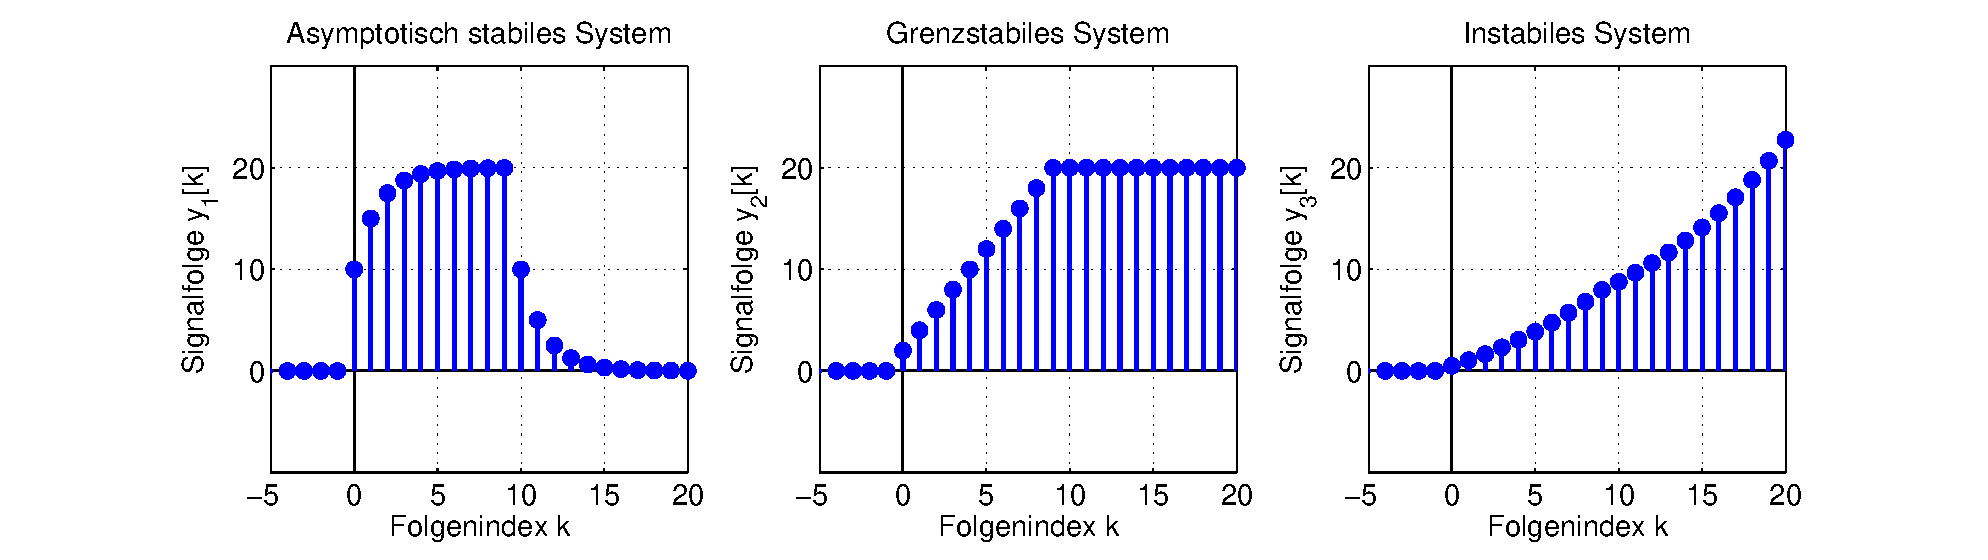
\includegraphics[width=1\textwidth]{Kapitel6/Bilder/image10.eps}}
  \caption{Lage der Pol- und Nullstellen sowie und Impulsantwort bei einfachen reellen Polen}
  \label{fig:SystemReellePole}
\end{figure}

\noindent Der Pol an der Stelle $\alpha_{1}$ = 0.5 liegt innerhalb des Einheitskreises, der korrespondierende Teil der Impulsantwort g${}_{1}$[k] ist konvergent. Der Pol an der Stelle $\alpha_{2}$ = 1.5 liegt au{\ss}erhalb des Einheitskreises und f\"{u}hrt zu einem divergenten Anteil g${}_{2}$[k] an der Impulsantwort. Die Summe der Impulsantworten ist damit divergent. Sobald ein Pol der \"{U}bertragungsfunktion au{\ss}erhalb des Einheitskreises liegt, divergiert die Impulsantwort, und das System ist instabil. Ausf\"{u}hrlich wird die Stabilit\"{a}t von Systemen in Abschnitt 6.3.11 diskutiert.

\subsubsection{\"{U}bertragungsfunktionen mit mehrfachen Polen}

\noindent Liegt ein N-facher Pol an der Stelle $\alpha$ $\neq$ 0 vor, ergibt sich f\"{u}r die Partialbruchzerlegung dieses Teils der \"{U}bertragungsfunktion der Ansatz

\begin{equation}\label{eq:sixsninetyfive}
G\left(z\right)=\frac{B\left(z\right)}{\left(z-\alpha \right)^{N} } =\sum _{n=1}^{N}\frac{A_{n} }{\left(z-\alpha \right)^{n} }
\end{equation}

\noindent Die R\"{u}cktransformation der einzelnen Summanden kann mit Korrespondenz 9 angegeben werden zu

\begin{equation}\label{eq:sixsninetysix}
g_{n} \left[k\right]=A_{n} \cdot \left(\begin{array}{c} {k-1} \\ {n-1} \end{array}\right)\cdot \alpha ^{k-n} \cdot \sigma \left[k-n\right]
\end{equation}

\noindent Zum Beispiel ergibt sich f\"{u}r einen zweifachen Pol

\begin{equation}\label{eq:sixsninetyseven}
g\left[k\right]=\sum _{n=1}^{2}A_{n} \cdot \left(\begin{array}{c} {k-1} \\ {n-1} \end{array}\right)\cdot \alpha ^{k-n} \cdot \sigma \left[k-n\right]=A_{1} \cdot \alpha ^{k-1} \cdot \sigma \left[k-1\right]+A_{2} \cdot \left(k-1\right)\cdot \alpha ^{k-2} \cdot \sigma \left[k-2\right]
\end{equation}

\noindent Die Impulsantwort ist unendlich lang, es handelt sich also um ein IIR-System. Der Ausdruck 

\begin{equation}\label{eq:sixsninetyeight}
\left(\begin{array}{l} {k-1} \\ {n-1} \end{array}\right)=\frac{\left(k-1\right)!}{\left(n-1\right)!\cdot \left(k-1-n+1\right)!} =\frac{\left(k-1\right)!}{\left(n-1\right)!\cdot \left(k-n\right)!}
\end{equation}

\noindent f\"{u}hrt zu einem Polynom in k mit der Ordnung n - 1. Da die Exponentialfunktion f\"{u}r $\alpha$ $\neq$ 1 st\"{a}rker steigt oder f\"{a}llt als jede Potenz von k, ist die Stabilit\"{a}tsbetrachtung von diesem Ausdruck unabh\"{a}ngig. Deshalb bestimmt auch in diesem Fall der Betrag des Pols $\alpha$, ob die Impulsantwort gegen den Wert null konvergiert, und entscheidet damit \"{u}ber die Stabilit\"{a}t des Systems. Der Sonderfall eines Pols mit dem Betrag 1 wird in Abschnitt 6.3.11 diskutiert.\bigskip

\noindent
\colorbox{lightgray}{%
\arrayrulecolor{white}%
\renewcommand\arraystretch{0.6}%
\begin{tabular}{ wl{16.5cm} }
{\fontfamily{phv}\selectfont{Beispiel: \"{U}bertragungsfunktion mit mehrfachen reellen Polen}}
\end{tabular}%
}\medskip

\noindent Die untenstehende \"{U}bertragungsfunktion G(z) soll interpretiert werden. Ihr Z\"{a}hlergrad ist kleiner als der Nennergrad, und sie hat einen doppelten Pol an der Stelle $\alpha$ = - 0.5. Es ergibt sich die Partialbruchzerlegung

\begin{equation}\label{eq:sixsninetynine}
G\left(z\right)=\frac{z+1}{\left(z+0.5\right)^{2} } =\frac{1}{z+0.5} +\frac{0.5}{\left(z+0.5\right)^{2} } =\frac{z}{z+0.5} \cdot z^{-1} -\frac{-0.5\cdot z}{\left(z+0.5\right)^{2} } \cdot z^{-1}
\end{equation}

\noindent Zur R\"{u}cktransformation werden die Korrespondenzen 5 und 6 sowie der Verschiebungssatz verwendet.

\begin{equation}\label{eq:sixsonehundred}
g\left[k\right]=g_{1} \left[k\right]+g_{2} \left[k\right]=\left(-0.5\right)^{k-1} \cdot \sigma \left[k-1\right]-(k-1)\cdot \left(-0.5\right)^{k-1} \cdot \sigma \left[k-2\right]
\end{equation}

\noindent In Bild \ref{fig:SystemDoppelteReellePole} sind die Lage der Nullstelle und Pole sowie die Impulsantwort des Systems dargestellt.

\begin{figure}[H]
  \centerline{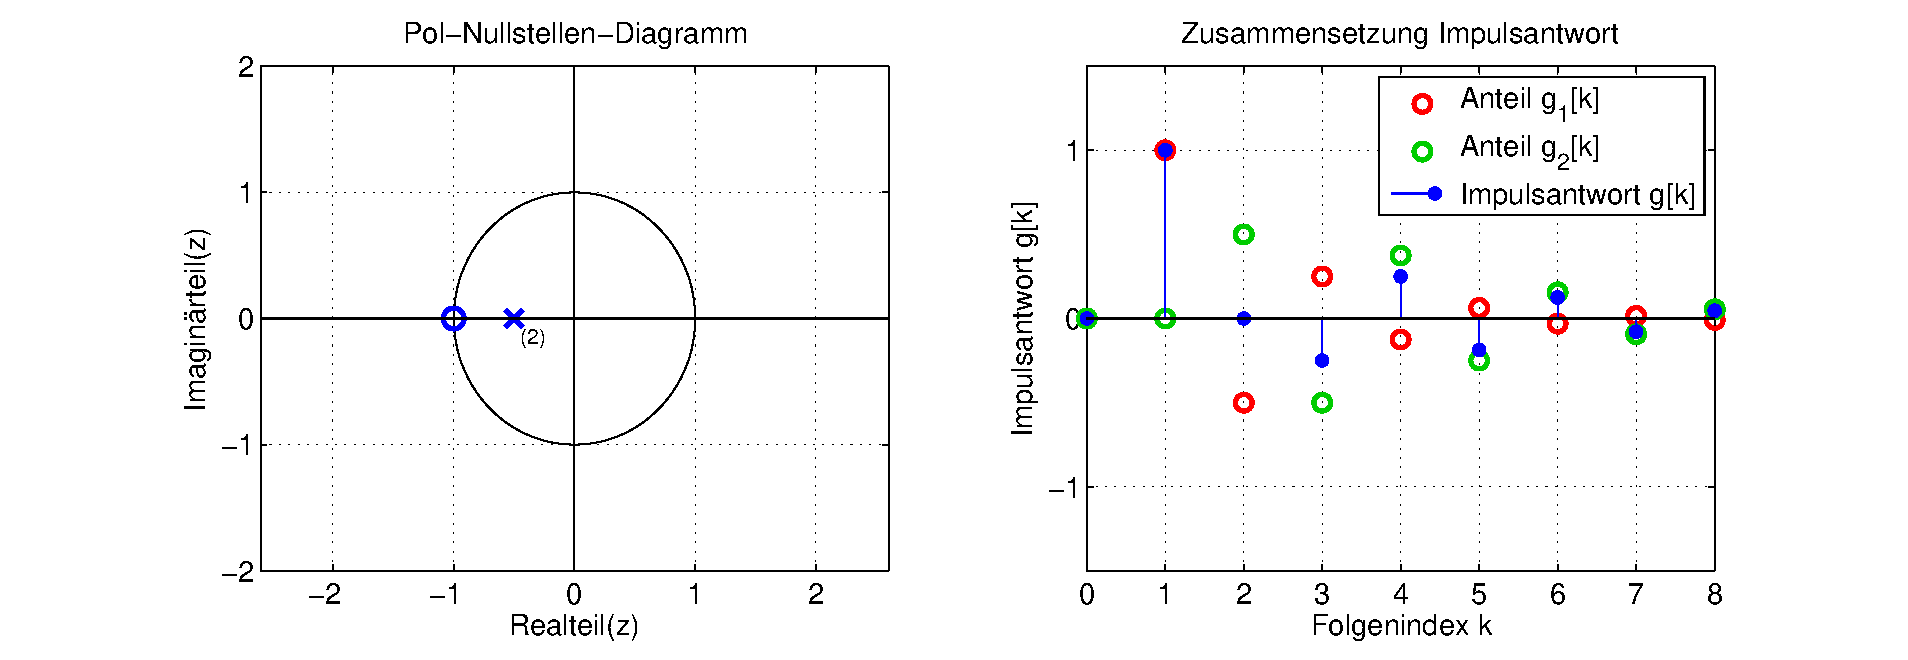
\includegraphics[width=1\textwidth]{Kapitel6/Bilder/image11.eps}}
  \caption{Lage der Nullstelle und Pole sowie die Impulsantwort bei mehrfachem reellenm Pol}
  \label{fig:SystemDoppelteReellePole}
\end{figure}

\noindent Da der mehrfache Pol innerhalb des Einheitskreises liegt, ist das System stabil. Aufgrund des negativen Vorzeichens sind die beiden Teile der Impulsantwort alternierend, und es ergibt sich eine schwingende Impulsantwort. Besitzt die \"{U}bertragungsfunktion einen einfachen oder mehrfachen Pol mit negativem Vorzeichen, 
\begin{equation}\label{eq:sixsonehundredone}
G\left(z\right)=\frac{z}{z-r_{0} \cdot e^{j\cdot \pi } }
\end{equation}

\noindent wechselt das Vorzeichen der Impulsantwort des zeitdiskreten Systems. Die Impulsantwort schwingt mit der normierten Kreisfrequenz $\pi$.

\begin{equation}\label{eq:sixsonehundredtwo}
g\left[k\right]=r_{0}^{k} \cdot e^{j\cdot \pi \cdot k} \cdot \sigma \left[k\right]=r_{0}^{k} \cdot \left(-1\right)^{k} \cdot \sigma \left[k\right]
\end{equation}

\noindent Diese Systemeigenschaft besitzt im zeitkontinuierlichen Bereich kein \"{A}quivalent.

\clearpage

\subsubsection{\"{U}bertragungsfunktion mit konjugiert komplexem Polpaar}

\noindent Im Fall konjugiert komplexer Polpaare weist die \"{U}bertragungsfunktion Partialbr\"{u}che der Form 

\begin{equation}\label{eq:sixsonehundredthree}
G\left(z\right)=\frac{A_{1} }{z-r\cdot e^{j\cdot \varphi } } +\frac{A_{2} }{z-r\cdot e^{-j\cdot \varphi } } =\frac{A}{z-r\cdot e^{j\cdot \varphi } } +\frac{A^{*} }{z-r\cdot e^{-j\cdot \varphi } } =\frac{A\cdot e^{j\cdot \varphi _{A} } }{z-r\cdot e^{j\cdot \varphi } } +\frac{A\cdot e^{-j\cdot \varphi _{A} } }{z-r\cdot e^{-j\cdot \varphi } }
\end{equation}

\noindent auf. Damit das System reelle Koeffizienten a${}_{n}$ und b${}_{m}$ besitzt, m\"{u}ssen die Koeffizienten der Partialbr\"{u}che A${}_{1}$ und A${}_{2}$ ebenfalls konjugiert komplex zueinander sein. Die Impulsantwort errechnet sich zu

\begin{equation}\label{eq:sixsonehundredfour}
\begin{split}
g\left[k\right] & = A\cdot e^{j\cdot \varphi _{A} } \cdot \left(r\cdot e^{j\cdot \varphi}\right)^{k-1} \cdot \sigma \left[k-1\right]+A\cdot e^{-j\cdot \varphi _{A} } \cdot\left(r\cdot e^{-j\cdot \varphi }\right)^{k-1} \cdot \sigma \left[k-1\right] \\ 
& = A\cdot r^{k-1} \left(e^{j\cdot \varphi _{A} } \cdot e^{j\cdot \varphi \cdot \left(k-1\right)} +e^{-j\cdot \varphi _{A} } \cdot e^{-j\cdot \varphi \cdot \left(k-1\right)} \right)\cdot \sigma \left[k-1\right] \\
&=2\cdot A\cdot r^{k-1} \cdot \cos \left(\varphi \cdot \left(k-1\right)+\varphi _{A} \right)\cdot \sigma \left[k-1\right]
\end{split}
\end{equation}

\noindent Die Folge ist eine ged\"{a}mpfte harmonische Folge. Die Phasenlage $\varphi$ des Polpaares definiert, mit welcher Frequenz die Folge schwingt. Der Betrag der Pole r ist f\"{u}r das Abfallen beziehungsweise Ansteigen der Amplitude verantwortlich. Die Koeffizienten A und A* bestimmen \"{u}ber die Amplitude und Phasenlage der Impulsantwort. Die Impulsantwort ist wieder unendlich lang, es handelt sich also erwartungsgem\"{a}{\ss} um ein IIR-System.\bigskip

\noindent
\colorbox{lightgray}{%
\arrayrulecolor{white}%
\renewcommand\arraystretch{0.6}%
\begin{tabular}{ wl{16.5cm} }
{\fontfamily{phv}\selectfont{Beispiel: \"{U}bertragungsfunktion mit konjugiert komplexem Polpaar}}
\end{tabular}%
}\medskip

\noindent Die z-Transformierte G(z) soll in den Zeitbereich zur\"{u}cktransformiert werden. Ihr Z\"{a}hlergrad ist kleiner als der Nennergrad, und sie hat ein konjugiert komplexes Polpaar an der Stelle $\alpha$ = + 0.5 $\pm$ 0.5$.$j. Es ergibt sich die Partialbruchzerlegung

\begin{equation}\label{eq:sixsonehundredfive}
G\left(z\right)=\frac{2\cdot z}{z^{2} -z+0.5} =\frac{1-j}{z-0.5-0.5\cdot j}+\frac{1+j}{z-0.5+0.5\cdot j}=\frac{\sqrt{2}\cdot e^{-j\cdot\pi/4}}{z-\frac{e^{j\cdot \pi /4} }{\sqrt{2} } } +\frac{\sqrt{2} \cdot e^{j\cdot\pi /4}}{z-\frac{e^{-j\cdot \pi /4} }{\sqrt{2}}}
\end{equation}

\noindent Die R\"{u}cktransformation f\"{u}hrt nach den Ausf\"{u}hrungen oben zu der Impulsantwort

\begin{equation}\label{eq:sixsonehundredsix}
g\left[k\right]=2\cdot \sqrt{2} \cdot \left(\frac{1}{\sqrt{2} } \right)^{k-1} \cdot \cos \left(\frac{\pi }{4} \cdot \left(k-1\right)-\frac{\pi }{4} \right)\cdot \sigma \left[k-1\right]
\end{equation}

\noindent In Bild \ref{fig:SystemKonjKomplexePole} sind die Lage der Pole und Nullstelle sowie die Impulsantwort des Systems dargestellt.

\begin{figure}[H]
  \centerline{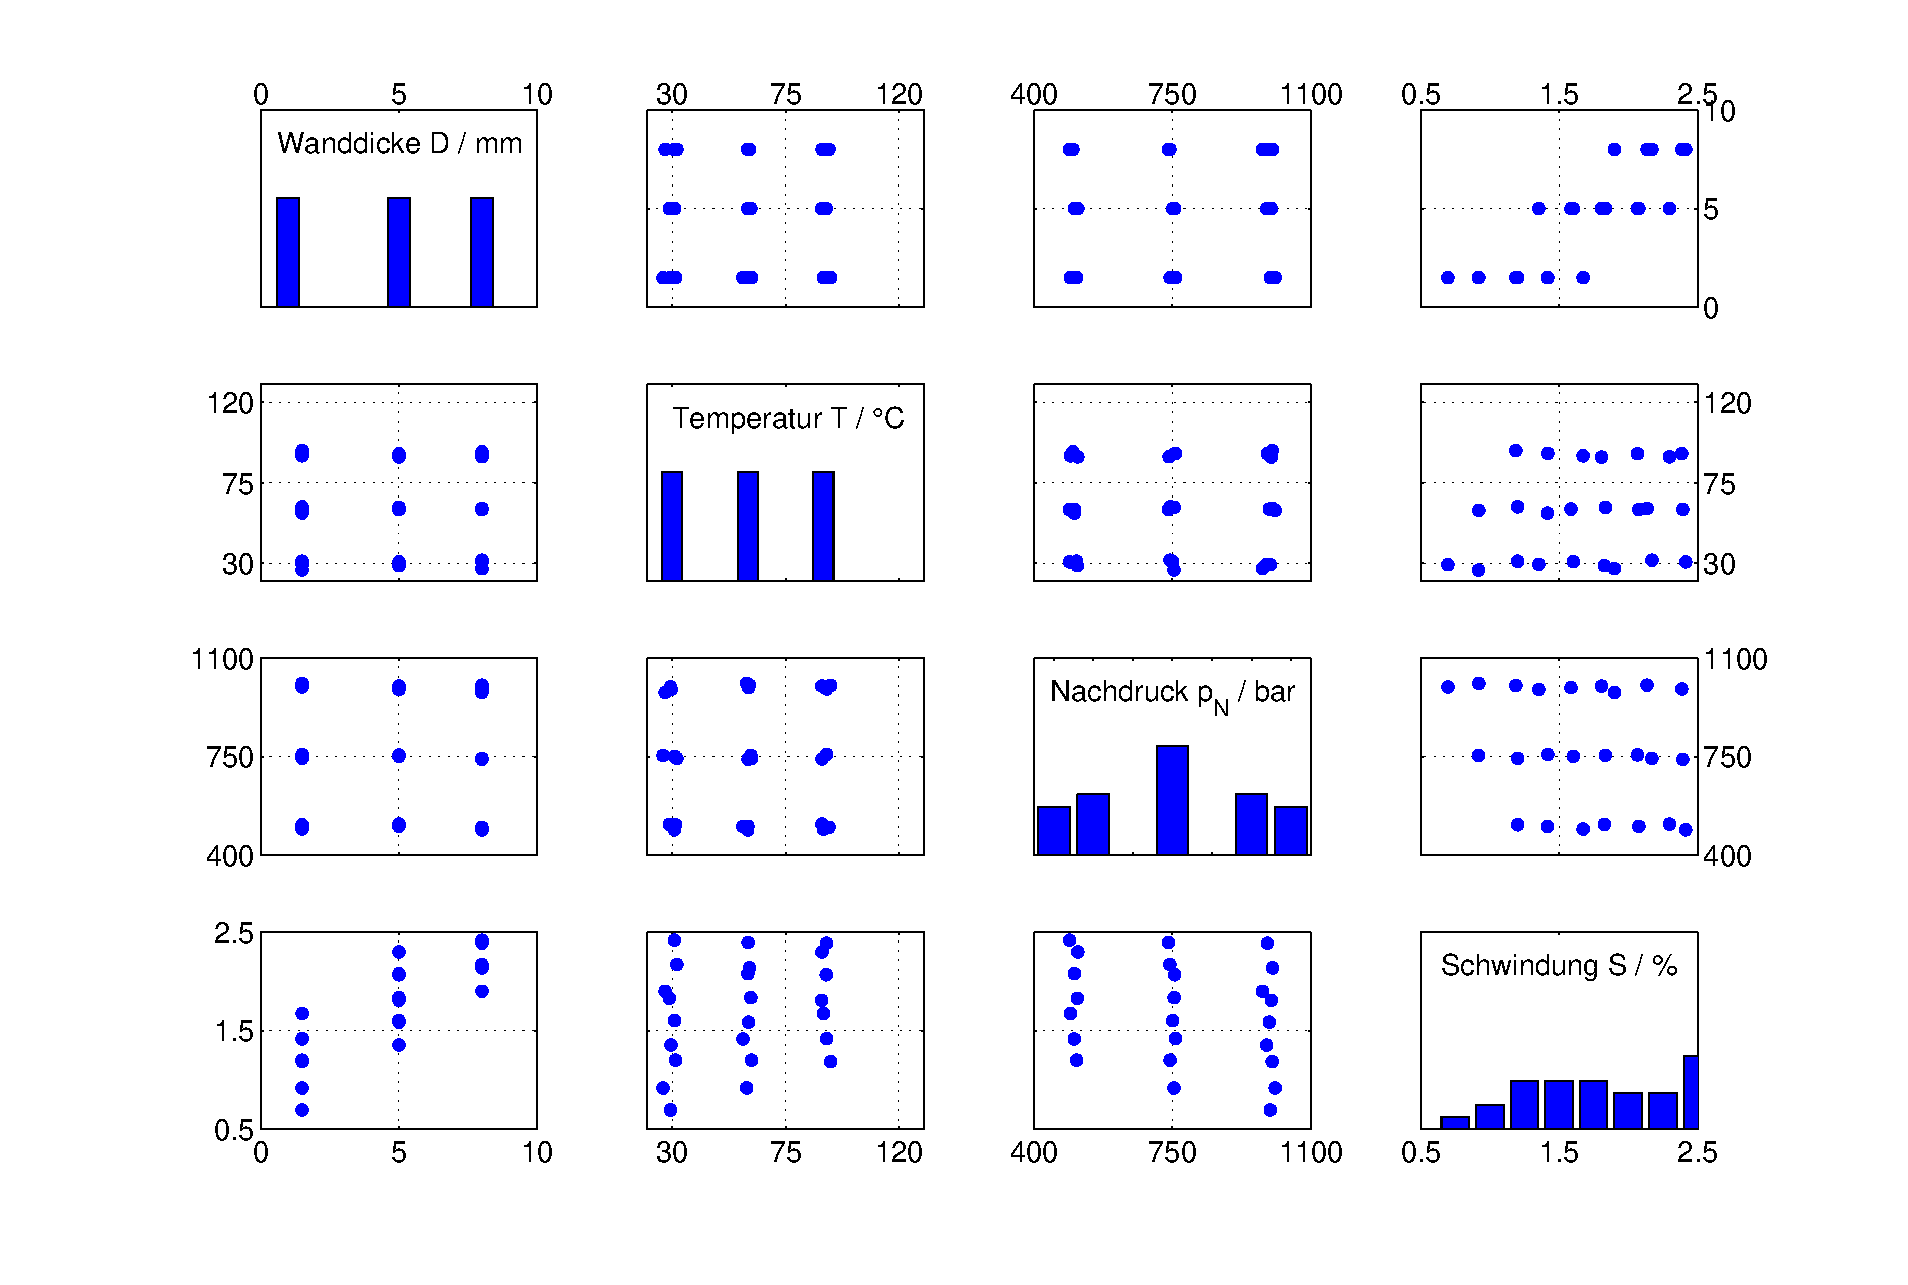
\includegraphics[width=1\textwidth]{Kapitel6/Bilder/image12.eps}}
  \caption{Lage der Nullstelle und Pole sowie die Impulsantwort bei konjugiert komplexem Polpaar}
  \label{fig:SystemKonjKomplexePole}
\end{figure}

\noindent Die Impulsantwort eines zeitdiskreten Systems mit konjugiert komplexem Polpaar schwingt. Liegen die Pole innerhalb des Einheitskreises nimmt die Amplitude der Schwingung ab.

\clearpage

\subsubsection{\"{U}bertragungsfunktion mit N-fachem Pol im Koordinatenursprung}

\noindent Wenn die \"{U}bertragungsfunktion G(z) nur Pole an der Stelle $\alpha$ = 0 besitzt, sind alle Koeffizienten a${}_{n}$ = 0 bis auf den Koeffizienten a${}_{N}$. Damit gilt

\begin{equation}\label{eq:sixsonehundredseven}
G\left(z\right)=\frac{\sum _{m=0}^{M}b_{m} \cdot z^{m}  }{a_{N} \cdot z^{N} } =\sum _{m=0}^{M}\frac{b_{m} }{a_{N} } \cdot z^{m-N}  =\frac{b_{0} }{a_{N} } \cdot z^{-N} +\frac{b_{1} }{a_{N} } \cdot z^{1-N} +...+\frac{b_{M} }{a_{N} } \cdot z^{M-N}
\end{equation}

\noindent Bei kausalen Systemen ist der Z\"{a}hlergrad M kleiner oder gleich dem Nennergrad N. Damit sind alle Exponenten der komplexen Variablen z kleiner oder gleich null, und es kann der Verschiebungssatz der z-Transformation angewendet werden. Die Impulsantwort ergibt sich damit zu

\begin{equation}\label{eq:sixsonehundredeight}
g\left[k\right]=\frac{b_{0} }{a_{N} } \cdot \delta \left[k-N\right]+\frac{b_{1} }{a_{N} } \cdot \delta \left[k-N+1\right]+...+\frac{b_{M} }{a_{N} } \cdot \delta \left[k-N+M\right]
\end{equation}

\noindent Die Impulsantwort besteht aus N + 1 Impulsen. Die Koeffizienten der Impulse entsprechen den Koeffizienten der \"{U}bertragungsfunktion G(z). Im Gegensatz zu den bisher behandelten Impulsantworten ist sie nur an N + 1 Stellen von null verschieden. Deshalb wird die Impulsantwort als Finite-Impulse-Response und die Systeme als Finite-Impulse-Response-Systeme (FIR-Systeme) bezeichnet.\bigskip

\noindent
\colorbox{lightgray}{%
\arrayrulecolor{white}%
\renewcommand\arraystretch{0.6}%
\begin{tabular}{ wl{16.5cm} }
{\fontfamily{phv}\selectfont{Beispiel: N-facher Pol im Koordinatenursprung}}
\end{tabular}%
}\medskip

\noindent Die \"{U}bertragungsfunktion G(z) soll in den Zeitbereich zur\"{u}cktransformiert werden. Sie hat einen 4-fachen Pol an der Stelle $\alpha$ = 0. Das System besitzt eine endliche Impulsantwort.

\begin{equation}\label{eq:sixsonehundrednine}
G\left(z\right)=\frac{z^{4} +2\cdot z^{3} +3\cdot z^{2} +2\cdot z+1}{9\cdot z^{4} } =\frac{1}{9} \cdot \left(1+2\cdot z^{-1} +3\cdot z^{-2} +2\cdot z^{-3} +1\cdot z^{-4} \right)
\end{equation}

\noindent Mit dem Verschiebungssatz der z-Transformation ergibt sich im Zeitbereich die Folge

\begin{equation}\label{eq:sixsonehundredten}
g\left[k\right]=\frac{1}{9} \cdot \delta \left[k\right]+\frac{2}{9} \cdot \delta \left[k-1\right]+\frac{3}{9} \cdot \delta \left[k-2\right]+\frac{2}{9} \cdot \delta \left[k-3\right]+\frac{1}{9} \cdot \delta \left[k-4\right]
\end{equation}

\noindent Die Werte der Impulsantwort sind identisch zu den Koeffizienten des Filters. In Bild \ref{fig:SystemPoleImUrsprung} sind die Lage der Pole und Nullstellen sowie die Impulsantwort des Systems dargestellt.

\begin{figure}[H]
  \centerline{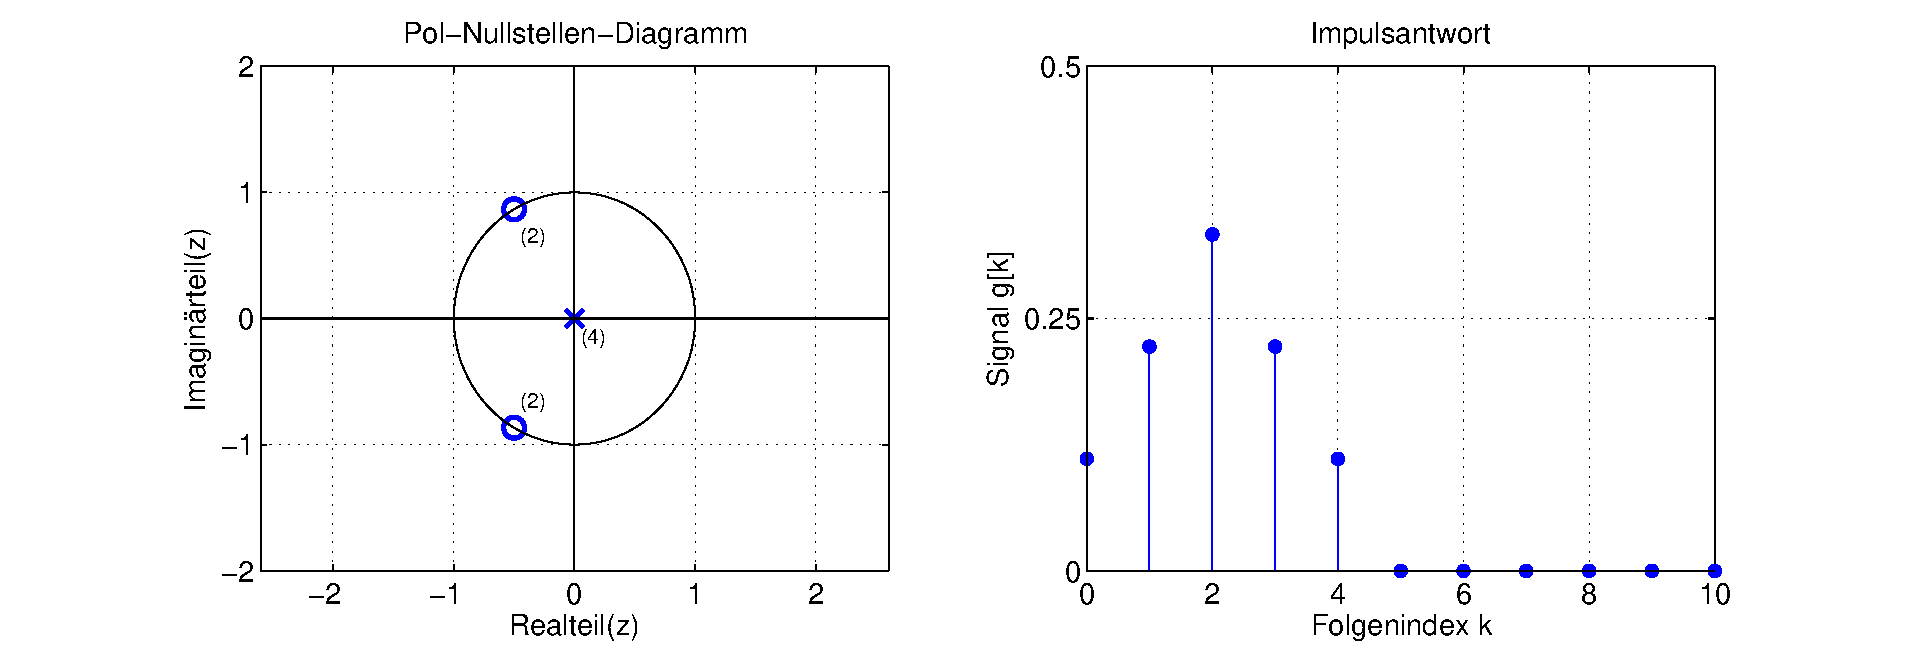
\includegraphics[width=1\textwidth]{Kapitel6/Bilder/image13.eps}}
  \caption{Pollage und Impulsantwort bei Polen im Koordinatenursprung}
  \label{fig:SystemPoleImUrsprung}
\end{figure}

\noindent Die Impulsantwort hat N + 1 = 5 von null verschiedene Werte. F\"{u}r k $\geq$ 5 bleibt die Impulsantwort null.

\subsubsection{\"{U}bertragungsfunktion invertierbarer Systeme}

\noindent Bei der \"{U}bertragung von Signalen ist es unter Umst\"{a}nden erforderlich, Verzerrungen einer \"{U}bertragungsstrecke zu kompensieren. Dazu wird ein System verwendet, das ein inverses Systemverhalten aufweist. Angenommen ein Signal wird \"{u}ber ein System G${}_{1}$(z) \"{u}bertragen, das die Form

\begin{equation}\label{eq:sixsonehundredeleven}
G_{1} \left(z\right)=\frac{z-\beta }{z-\alpha}
\end{equation}

\noindent aufweist. Zur Kompensation wird ein System verwendet, das im Idealfall folgende Bedingung erf\"{u}llt

\begin{equation}\label{eq:sixsonehundredtwelve}
G_{1} \left(z\right)\cdot G_{2} \left(z\right)=1
\end{equation}

\noindent In diesem Fall w\"{u}rden die Verzerrungen, die durch die Signal\"{u}bertragung im System G${}_{1}$(z) entstanden sind, ideal kompensiert. Aufl\"{o}sen der Bedingung f\"{u}hrt zu der \"{U}bertragungsfunktion

\begin{equation}\label{eq:sixsonehundredthirteen}
G_{2} \left(z\right)=\frac{1}{G_{1} \left(z\right)} =\frac{1}{\frac{z-\beta }{z-\alpha } } =\frac{z-\alpha }{z-\beta}
\end{equation}

\noindent Die Nullstellen der \"{U}bertragungsfunktion G${}_{1}$(z) werden zu Polen der inversen \"{U}bertragungsfunktion G${}_{2}$(z). Das inverse System G${}_{2}$(z) muss stabil sein, damit es realisierbar ist. Damit darf ein System, dessen Verhalten kompensiert werden soll, nur Nullstellen innerhalb des Einheitskreises besitzen. Bild \ref{fig:SystemInvertierbar} zeigt ein Beispiel f\"{u}r die Pol- und Nullstellenlage invertierbarer und nicht invertierbarer Systeme.

\begin{figure}[H]
  \centerline{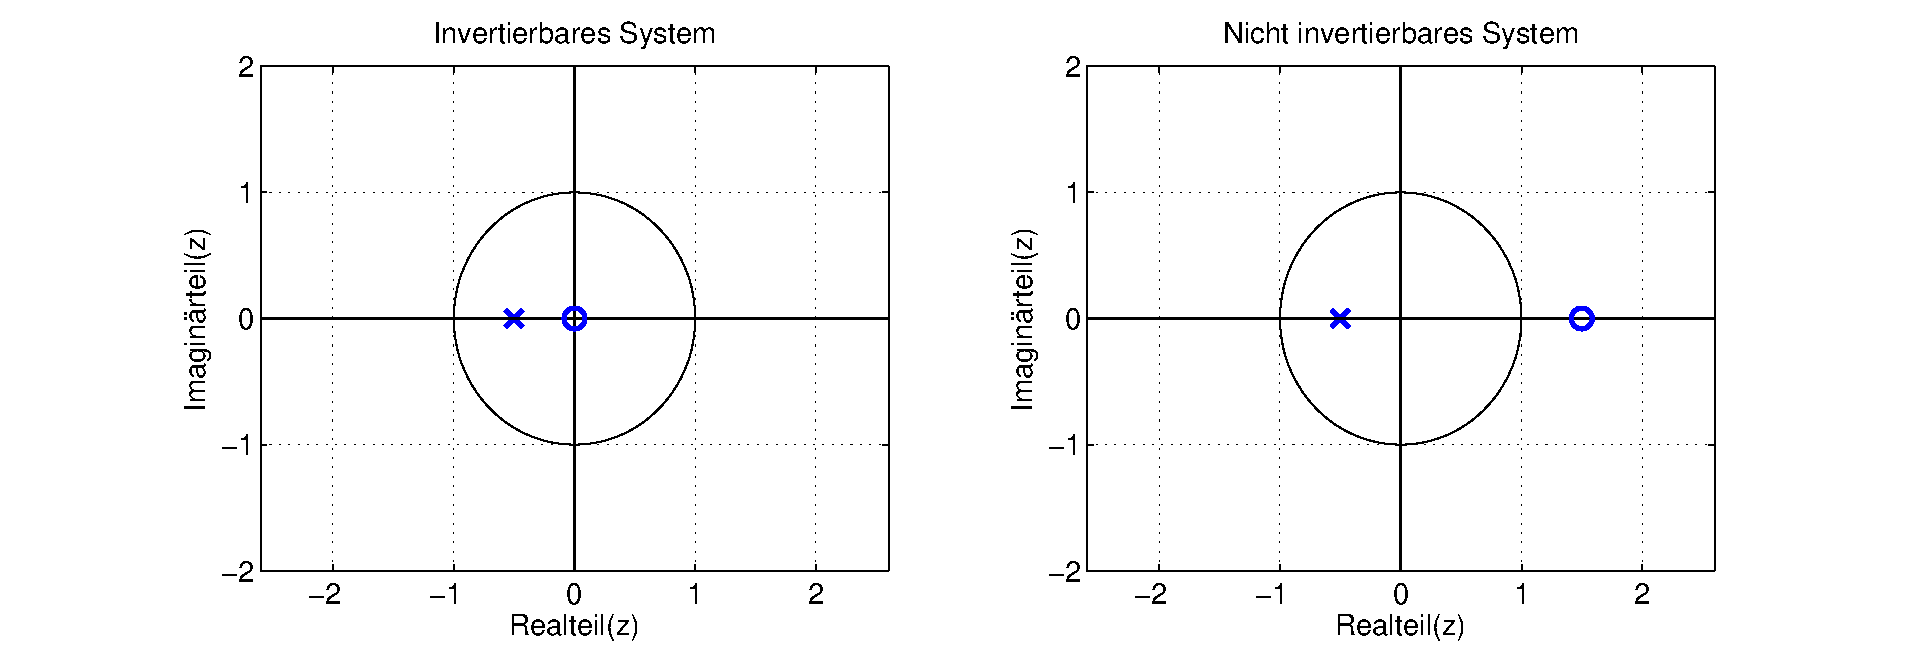
\includegraphics[width=1\textwidth]{Kapitel6/Bilder/image14.eps}}
  \caption{Pollage f\"{u}r ein invertierbares und ein nicht invertierbares System}
  \label{fig:SystemInvertierbar}
\end{figure}

\noindent Beide Systeme sind stabil, da der Pol bei beiden Systemen im Einheitskreis liegt. Das linke System ist invertierbar, da die Nullstelle innerhalb des Einheitskreises liegt. Das rechte System ist wegen der Lage der Nullstelle au{\ss}erhalb des Einheitskreises nicht invertierbar.
\clearpage
\subsubsection{Zusammenfassung Interpretation der \"{U}bertragungsfunktion}

\noindent Bei der Interpretation von \"{U}bertragungsfunktionen werden unterschiedliche Systemeigenschaften aufgezeigt. Tabelle \ref{tab:sixfour} fasst die an der \"{U}bertragungsfunktion ablesbaren Systemeigenschaften zusammen. Der Zusammenhang zwischen Pollage und Impulsantwort ist f\"{u}r einfache reelle Pole und f\"{u}r konjugiert komplexe Polpaare in Tabelle \ref{tab:sixfive} dargestellt.

\begin{table}[H]
\setlength{\arrayrulewidth}{.1em}
\caption{Tabellarische \"{U}bersicht der an der \"{U}bertragungsfunktion ablesbaren Systemeigenschaften}
\setlength{\fboxsep}{0pt}%
\colorbox{lightgray}{%
\arrayrulecolor{white}%
\begin{tabular}{| c | c |}
\hline
\parbox[c][0.35in][c]{3.3in}{\smallskip\centering\textbf{\fontfamily{phv}\selectfont{Eigenschaft}}} & 
\parbox[c][0.35in][c]{3.3in}{\smallskip\centering\textbf{\fontfamily{phv}\selectfont{Übertragungsfunktion}}}\\ \hline

\parbox[c][0.4in][c]{3.3in}{\centering{\fontfamily{phv}\selectfont{Kausalität}}} & 
\parbox[c][0.4in][c]{3.3in}{\centering{\fontfamily{phv}\selectfont{Z\"{a}hlergrad M $\leq$ Nennergrad N}}}\\ \hline

\parbox[c][0.4in][c]{3.3in}{\centering{\fontfamily{phv}\selectfont{Sprungfähigkeit}}} & 
\parbox[c][0.4in][c]{3.3in}{\centering\fontfamily{phv}\selectfont{{Z\"{a}hlergrad M = Nennergrad N}}}\\ \hline

\parbox[c][0.4in][c]{3.3in}{\centering{\fontfamily{phv}\selectfont{Schwingungsneigung}}} & 
\parbox[c][0.4in][c]{3.3in}{\centering{\fontfamily{phv}\selectfont{negative reelle Pole oder konjugiert komplexe Polpaare}}}\\ \hline

\parbox[c][0.5in][c]{3.3in}{\centering{\fontfamily{phv}\selectfont{System mit endlicher Impulsantwort\\
Finite-Impulse-Response (FIR-System)}}} & 
\parbox[c][0.5in][c]{3.3in}{\centering{\fontfamily{phv}\selectfont{Alle Pole im Koordinatenursprung}}}\\ \hline

\parbox[c][0.5in][c]{3.3in}{\centering{\fontfamily{phv}\selectfont{System mit unendlicher Impulsantwort\\
Infinite-Impulse-Response (IIR-System)}}} & 
\parbox[c][0.5in][c]{3.3in}{\centering{\fontfamily{phv}\selectfont{Mindestens ein Pol nicht \\
im Koordinatenursprung}}}\\ \hline

\parbox[c][0.5in][c]{3.3in}{\centering{\fontfamily{phv}\selectfont{Stabile invertierbare Systeme}}} & 
\parbox[c][0.5in][c]{3.3in}{\centering{\fontfamily{phv}\selectfont{Pole und Nullstellen innerhalb des Einheitskreises,
Zählergrad M = Nennergrad N}}}\\ \hline

\parbox[c][0.4in][c]{3.3in}{\centering{\fontfamily{phv}\selectfont{Verstärkung}}} & 
\parbox[c][0.4in][c]{3.3in}{\centering{\fontfamily{phv}\selectfont{Übertragungsfunktion $G(z = 1)$}}}\\ \hline

\end{tabular}%
}
\label{tab:sixsix}
\end{table}

\clearpage

\begin{table}[H]
\setlength{\arrayrulewidth}{.1em}
\caption{Tabellarische \"{U}bersicht \"{u}ber korrespondierende Elemente der s- und z-Ebene}
\setlength{\fboxsep}{0pt}%
\colorbox{lightgray}{%
\arrayrulecolor{white}%
\begin{tabular}{| c | c |}
\hline
\parbox[c][0.35in][c]{3.3in}{\smallskip\centering\textbf{\fontfamily{phv}\selectfont{Pollage X(z)}}} & \parbox[c][0.35in][c]{3.3in}{\smallskip\centering\textbf{\fontfamily{phv}\selectfont{Signalfolge x[k]}}}\\ \hline

\parbox[c][1.4in][c]{3.3in}{\centerline{\includegraphics[width=0.3\textwidth]{Kapitel6/Table/image1.png}}} & 
\parbox[c][1.4in][c]{3.3in}{\centerline{\includegraphics[width=0.3\textwidth]{Kapitel6/Table/image2.png}}}\\ \hline

\parbox[c][1.4in][c]{3.3in}{\centerline{\includegraphics[width=0.3\textwidth]{Kapitel6/Table/image3.png}}} & 
\parbox[c][1.4in][c]{3.3in}{\centerline{\includegraphics[width=0.3\textwidth]{Kapitel6/Table/image4.png}}}\\ \hline

\parbox[c][1.4in][c]{3.3in}{\centerline{\includegraphics[width=0.3\textwidth]{Kapitel6/Table/image5.png}}} & 
\parbox[c][1.4in][c]{3.3in}{\centerline{\includegraphics[width=0.3\textwidth]{Kapitel6/Table/image6.png}}}\\ \hline

\parbox[c][1.4in][c]{3.3in}{\centerline{\includegraphics[width=0.3\textwidth]{Kapitel6/Table/image7.png}}} & 
\parbox[c][1.4in][c]{3.3in}{\centerline{\includegraphics[width=0.3\textwidth]{Kapitel6/Table/image8.png}}}\\ \hline

\parbox[c][1.4in][c]{3.3in}{\centerline{\includegraphics[width=0.3\textwidth]{Kapitel6/Table/image9.png}}} & 
\parbox[c][1.4in][c]{3.3in}{\centerline{\includegraphics[width=0.3\textwidth]{Kapitel6/Table/image10.png}}}\\ \hline

\parbox[c][1.4in][c]{3.3in}{\centerline{\includegraphics[width=0.3\textwidth]{Kapitel6/Table/image11.png}}} & 
\parbox[c][1.4in][c]{3.3in}{\centerline{\includegraphics[width=0.3\textwidth]{Kapitel6/Table/image12.png}}}\\ \hline


\end{tabular}%
}
\label{tab:sixseven}
\end{table}
\clearpage
\subsubsection{Stabilit\"{a}t und Pole der \"{U}bertragungsfunktion}

\noindent Bei der Einf\"{u}hrung des Begriffes der Stabilit\"{a}t in Abschnitt 4.4.4 wird gezeigt, dass asymptotisch stabile Systeme eine abklingende Impulsantwort aufweisen m\"{u}ssen. Die \"{U}bertragungsfunktion G(z) ist die z-Transformierte der Impulsantwort g[k]. Deshalb kann die Stabilit\"{a}tsbetrachtung auch im z-Bereich erfolgen. Liegen ausschlie{\ss}lich Pole mit einem Betrag {\textbar}$\alpha_{n}${\textbar} $\mathrm{<}$ 1 vor, konvergiert die Impulsantwort g[k] f\"{u}r k $\rightarrow$ $\infty$ gegen null. Das System ist asymptotisch stabil. Liegt mindestens ein Pol mit einem Betrag {\textbar}$\alpha_{n}${\textbar} $\mathrm{<}$ 1 vor, divergiert die Impulsantwort. Das System ist instabil. Bei einem Pol mit einem Betrag {\textbar}$\alpha${\textbar} = 1 entscheidet die Mehrfachheit \"{u}ber die Konvergenz. Zu der \"{U}bertragungsfunktion

\begin{equation}\label{eq:sixsonehundredfourteen}
G\left(z\right)=\frac{B\left(z\right)}{\left(z-e^{j\cdot \varphi } \right)^{N} } =\sum _{n=1}^{N}\frac{A_{n} }{\left(z-e^{j\cdot \varphi } \right)^{n} }
\end{equation}

\noindent geh\"{o}rt die Impulsantwort

\begin{equation}\label{eq:sixsonehundredfifteen}
g\left[k\right]=\sum _{n=1}^{N}A_{n} \cdot \left(\begin{array}{c} {k-1} \\ {n-1} \end{array}\right)\cdot e^{j\cdot \varphi \cdot \left(k-n\right)} \cdot \sigma \left[k-n\right]
\end{equation}

\noindent Der Binomialkoeffizient zum Beispiel f\"{u}r n = 2 zu einem Faktor

\begin{equation}\label{eq:sixsonehundredsixteen}
\left(\begin{array}{c} {k-1} \\ {2-1} \end{array}\right)=\frac{\left(k-1\right)!}{\left(2-1\right)!\, \cdot \left(k-2\right)!} =\left(k-1\right)
\end{equation}

\noindent Der Faktor steigt linear mit dem Folgenindex k. Er wird mit einer Exponentialfunktion multipliziert, deren Betrag konstant ist. Damit divergiert die Impulsantwort f\"{u}r eine Vielfachheit N $\geq$ 2.\bigskip

\noindent
\colorbox{lightgray}{%
\arrayrulecolor{white}%
\renewcommand\arraystretch{0.6}%
\begin{tabular}{ wl{16.5cm} }
{\fontfamily{phv}\selectfont{Beispiel: Stabilit\"{a}tsnachweis \"{u}ber Pollage}}
\end{tabular}%
}\medskip

\noindent Ein System mit der \"{U}bertragungsfunktion 

\begin{equation}\label{eq:sixsonehundredseventeen}
G\left(z\right)=\frac{1}{z^{3} +0.1\cdot z^{2} -0.25\cdot z-0.025}
\end{equation}

\noindent soll auf Stabilit\"{a}t gepr\"{u}ft werden. Die \"{U}bertragungsfunktion des Systems kann in Linearfaktorschreibweise dargestellt werden.

\begin{equation}\label{eq:sixsonehundredeighteen}
G\left(z\right)=\frac{1}{\left(z+0.5\right)\cdot \left(z+0.1\right)\cdot \left(z-0.5\right)}
\end{equation}

\noindent Alle Pole weisen einen Betrag r $\mathrm{<}$ 1 auf, das System ist damit stabil.\bigskip

\noindent
\colorbox{lightgray}{%
\arrayrulecolor{white}%
\renewcommand\arraystretch{0.6}%
\begin{tabular}{ wl{16.5cm} }
{\fontfamily{phv}\selectfont{Beispiel: Stabilit\"{a}tspr\"{u}fung eines Systems mit doppeltem Pol}}
\end{tabular}%
}\medskip

\noindent Ein System mit der \"{U}bertragungsfunktion 

\begin{equation}\label{eq:sixsonehundrednineteen}
G\left(z\right)=\frac{1}{\left(z-0.2\right)\cdot \left(z+1\right)^{2} }
\end{equation}

\noindent weist einen Pol an der Stelle $\alpha_{1}$ = 0.2 und einen doppelten Pol an der Stelle $\alpha_{2}$ = - 1 auf. Es ergeben sich die Partialbruchdarstellung

\begin{equation}\label{eq:sixsonehundredtwenty}
G\left(z\right)=\frac{1}{\left(z-0.2\right)\cdot \left(z+1\right)^{2}} =\frac{0.6944}{z-0.2} -\frac{0.6944}{z+1} +\frac{1.25}{\left(z+1\right)^{2}}
\end{equation}

\noindent und die Impulsantwort

\begin{equation}\label{eq:sixsonehundredtwentyone}
g\left[k\right]=0.6944\cdot 0.2^{k-1} \cdot \sigma \left[k-1\right]-0.6944\cdot \left(-1\right)^{k-1} \cdot \sigma \left[k-1\right]+1.25\cdot \left(k-1\right)\cdot \left(-1\right)^{k-1} \cdot \sigma \left[k-1\right]
\end{equation}

\noindent Wegen des letzten Summenden divergiert die Impulsantwort. Er ergibt sich aus dem doppelten Pol $\alpha_{2}$ mit einem Betrag von {\textbar}$\alpha_{2}${\textbar} = 1. Das System ist instabil.

\noindent Die Analyse der Pollage f\"{u}hrt zu einer Stabilit\"{a}tsbewertung, die in Tabelle \ref{tab:sixsix} zusammengefasst ist. Unter Ber\"{u}cksichtigung der in Bild 5.2 gezeigten Abbildung vom Laplace-Bereich in den z-Bereich entsprechen die Stabilit\"{a}tskriterien denen zeitkontinuierlicher Systeme im Laplace-Bereich.

\begin{table}[H]
\setlength{\arrayrulewidth}{.1em}
\caption{Zusammenhang zwischen Polen der \"{U}bertragungsfunktion und der Stabilit\"{a}t von zeitdiskreten LTI-Systemen, die sich \"{u}ber lineare Differenzengleichungen mit konstanten Koeffizienten beschreiben lassen }
\setlength{\fboxsep}{0pt}%
\colorbox{lightgray}{%
\arrayrulecolor{white}%
\begin{tabular}{| c | c |}
\hline
\parbox[c][0.35in][c]{3.3in}{\smallskip\centering\textbf{\fontfamily{phv}\selectfont{Eigenschaft}}} & 
\parbox[c][0.35in][c]{3.3in}{\smallskip\centering\textbf{\fontfamily{phv}\selectfont{Pole $\alpha_{n}$ der \"{U}bertragungsfunktion}}}\\ \hline

\parbox[c][0.4in][c]{3.3in}{\centering{\fontfamily{phv}\selectfont{Asymptotisch stabiles System}}} & 
\parbox[c][0.4in][c]{3.3in}{\centering{\fontfamily{phv}\selectfont{Alle Pole $\alpha_{n}$ besitzen einen Betrag {\textbar}$\alpha{}_{n}${\textbar} $\mathrm{<}$ 1}}}\\ \hline

\parbox[c][0.8in][c]{3.3in}{\centering{\fontfamily{phv}\selectfont{Grenzstabiles System}}} & 
\parbox[c][0.8in][c]{3.3in}{\centering{\fontfamily{phv}\selectfont{Alle L\"{o}sungen $\alpha_{n}$ besitzen einen Betrag {\textbar}$\alpha_{n}${\textbar} $\mathrm{<}$ 1, zus\"{a}tzlich liegt mindestens eine einfache L\"{o}sung mit Betrag {\textbar}$\alpha_{n}${\textbar} = 1 vor}}}\\ \hline

\parbox[c][0.8in][c]{3.3in}{\centering{\fontfamily{phv}\selectfont{Instabiles System}}} & 
\parbox[c][0.8in][c]{3.3in}{\centering{\fontfamily{phv}\selectfont{Es existiert mindestens eine L\"{o}sung $\alpha_{n}$ mit einem Betrag {\textbar}$\alpha_{n}${\textbar} $\mathrm{>}$ 1oder eine mehrfache L\"{o}sung mit Betrag {\textbar}$\alpha_{n}${\textbar} = 1}}}\\ \hline

\end{tabular}%
}
\label{tab:sixeight}
\end{table}

\noindent Diese Diskussion der Pollage entspricht der Diskussion von L\"{o}sungen der charakteristischen Gleichung in Abschnitt 4.3.3. Bei der Pollage werden die Pole der \"{U}bertragungsfunktion bestimmt:

\begin{equation}\label{eq:sixsonehundredtwentytwo}
\alpha ^{N} +a_{1} \cdot \alpha ^{N-1} +a_{2} \cdot \alpha ^{N-2} +...+a_{N} =0
\end{equation}

\noindent In Abschnitt 4.3.3 werden die L\"{o}sungen der charakteristischen Gleichung analysiert.

\begin{equation}\label{eq:sixsonehundredtwentythree}
\lambda ^{N} +a_{1} \cdot \lambda ^{N-1} +a_{2} \cdot \lambda ^{N-2} +...+a_{N} =0
\end{equation}

\noindent Unter der Annahme, dass in der \"{U}bertragungsfunktion keine gemeinsamen Pole und Nullstellen auftreten, sind beide Gleichungen identisch, sodass die Diskussion der L\"{o}sungen zu identischen Aussagen f\"{u}hren muss. Damit haben aber auch beide Gleichungen das Problem, dass sie nur f\"{u}r Systeme mit einer Ordnung N = 3 analytisch gel\"{o}st werden k\"{o}nnen. F\"{u}r Ordnungen N $\mathrm{>}$ 3 kann eine L\"{o}sung nur numerisch bestimmt werden. 

\clearpage

\subsection{Analyse und Simulation zeitdiskreter Systeme mit MATLAB}

\subsubsection{Interpretation der \"{U}bertragungsfunktion mit MATLAB}

\noindent Neben den MATLAB-Funktionen, die bei der z-Transformation behandelt werden, bietet MATLAB die M\"{o}glichkeit, eine \"{U}bertragungsfunktion im z-Bereich zu definieren und zu interpretieren. Tabelle \ref{tab:sixseven} stellt einige MATLAB-Befehle zur Interpretation von \"{U}bertragungsfunktionen zusammen. Dabei wird bei der \"{U}bertragungsfunktion von folgender Darstellungsform ausgegangen:

\begin{equation}\label{eq:sixsonehundredtwentyfour}
G\left(z\right)=\frac{Y\left(z\right)}{X\left(z\right)} =\frac{\sum _{m=0}^{N}b_{m} \cdot z^{m}}{\sum _{n=0}^{N}a_{n} \cdot z^{n}}
\end{equation}

\begin{table}[H]
\setlength{\arrayrulewidth}{.1em}
\caption{Tabellarische \"{U}bersicht \"{u}ber Befehle zur Interpretation von \"{U}bertragungsfunktionen in MATLAB}
\setlength{\fboxsep}{0pt}%
\colorbox{lightgray}{%
\arrayrulecolor{white}%
\begin{tabular}{| c | c |}
\hline
\parbox[c][0.35in][c]{2.5in}{\smallskip\centering\textbf{\fontfamily{phv}\selectfont{Befehl}}} & \parbox[c][0.35in][c]{4in}{\smallskip\centering\textbf{\fontfamily{phv}\selectfont{Beschreibung}}}\\ \hline

\parbox[c][0.4in][c]{2.5in}{\centering{\fontfamily{phv}\selectfont{G = tf([bM {\dots} b0],[aN {\dots} a0],TA);}}} & 
\parbox[c][0.4in][c]{4in}{\centering{\fontfamily{phv}\selectfont{Definition der Übertragungsfunktion über\\ 
Zähler- und Nennerpolynom sowie der Abtastzeit TA}}}\\ \hline

\parbox[c][0.4in][c]{2.5in}{\centering{\fontfamily{phv}\selectfont{zero(G)}}} & 
\parbox[c][0.4in][c]{4in}{\centering{\fontfamily{phv}\selectfont{Berechnung der Nullstellen der Übertragungsfunktion}}}\\ \hline

\parbox[c][0.4in][c]{2.5in}{\centering{\fontfamily{phv}\selectfont{pole(G)}}} & 
\parbox[c][0.4in][c]{4in}{\centering{\fontfamily{phv}\selectfont{Berechnung der Pole der Übertragungsfunktion}}}\\ \hline

\parbox[c][0.4in][c]{2.5in}{\centering{\fontfamily{phv}\selectfont{pzmap(G)}}} & 
\parbox[c][0.4in][c]{4in}{\centering{\fontfamily{phv}\selectfont{Darstellung der Pole und Nullstellen in der z-Ebene}}}\\ \hline

\parbox[c][0.4in][c]{2.5in}{\centering{\fontfamily{phv}\selectfont{impulse(G)}}} & 
\parbox[c][0.4in][c]{4in}{\centering{\fontfamily{phv}\selectfont{Berechnung / Darstellung der Impulsantwort}}}\\ \hline

\parbox[c][0.4in][c]{2.5in}{\centering{\fontfamily{phv}\selectfont{step(G)}}} & 
\parbox[c][0.4in][c]{4in}{\centering{\fontfamily{phv}\selectfont{Berechnung / Darstellung der Sprungantwort}}}\\ \hline

\end{tabular}%
}
\label{tab:sixnine}
\end{table}

\noindent Einige dieser Funktionen haben Erweiterungen, die sich aus der MATLAB-Hilfe ergeben und die hier nicht detailliert dargestellt werden sollen. \bigskip

\noindent
\colorbox{lightgray}{%
\arrayrulecolor{white}%
\renewcommand\arraystretch{0.6}%
\begin{tabular}{ wl{16.5cm} }
{\fontfamily{phv}\selectfont{Beispiel: Interpretation der Übertragungsfunktion mit MATLAB}}
\end{tabular}%
}\medskip

\noindent Zur Interpretation der Übertragungsfunktion mit MATLAB wird das Beispiel einer Übertragungsfunktion mit konjugiert komplexen Polstellen aufgegriffen, um die MATLAB-Ergebnisse mit den analytisch berechneten Ergebnissen vergleichen zu können. Die Übertragungsfunktion lautet:

\begin{equation}\label{eq:sixsonehundredtwentyfive}
G\left(z\right)=\frac{2\cdot z}{z^{2} -z+0.5}
\end{equation}

\noindent Die Definition erfolgt \"{u}ber die Koeffizienten von Z\"{a}hler- und Nennerpolynom, die jeweils als Vektor dargestellt werden. Dabei ist zu beachten, dass MATLAB die Koeffizienten der h\"{o}chsten Potenz von z als ersten Wert erwartet. Um MATLAB anzuzeigen, dass es sich um ein zeitdiskretes System handelt, wird die Abtastzeit als dritter Parameter angegeben. Hier wird die Abtastzeit T${}_{A}$ = 1 gew\"{a}hlt.

\clearpage

\lstinputlisting[caption = {}]{Kapitel6/mat1.m}

\noindent Ist die Übertragungsfunktion definiert, können Pole und Nullstellen berechnet werden. Weiterhin ist die Darstellung der Pole und Nullstellen in der z-Ebene möglich.

\lstinputlisting[caption = {}]{Kapitel6/mat2.m}

\noindent Mit diesen Befehlen gibt MATLAB die Pole und Nullstellen an und stellt sie wie in Bild \ref{fig:SystemInterpretationMatlab} als Grafik dar. 

\begin{figure}[H]
  \centerline{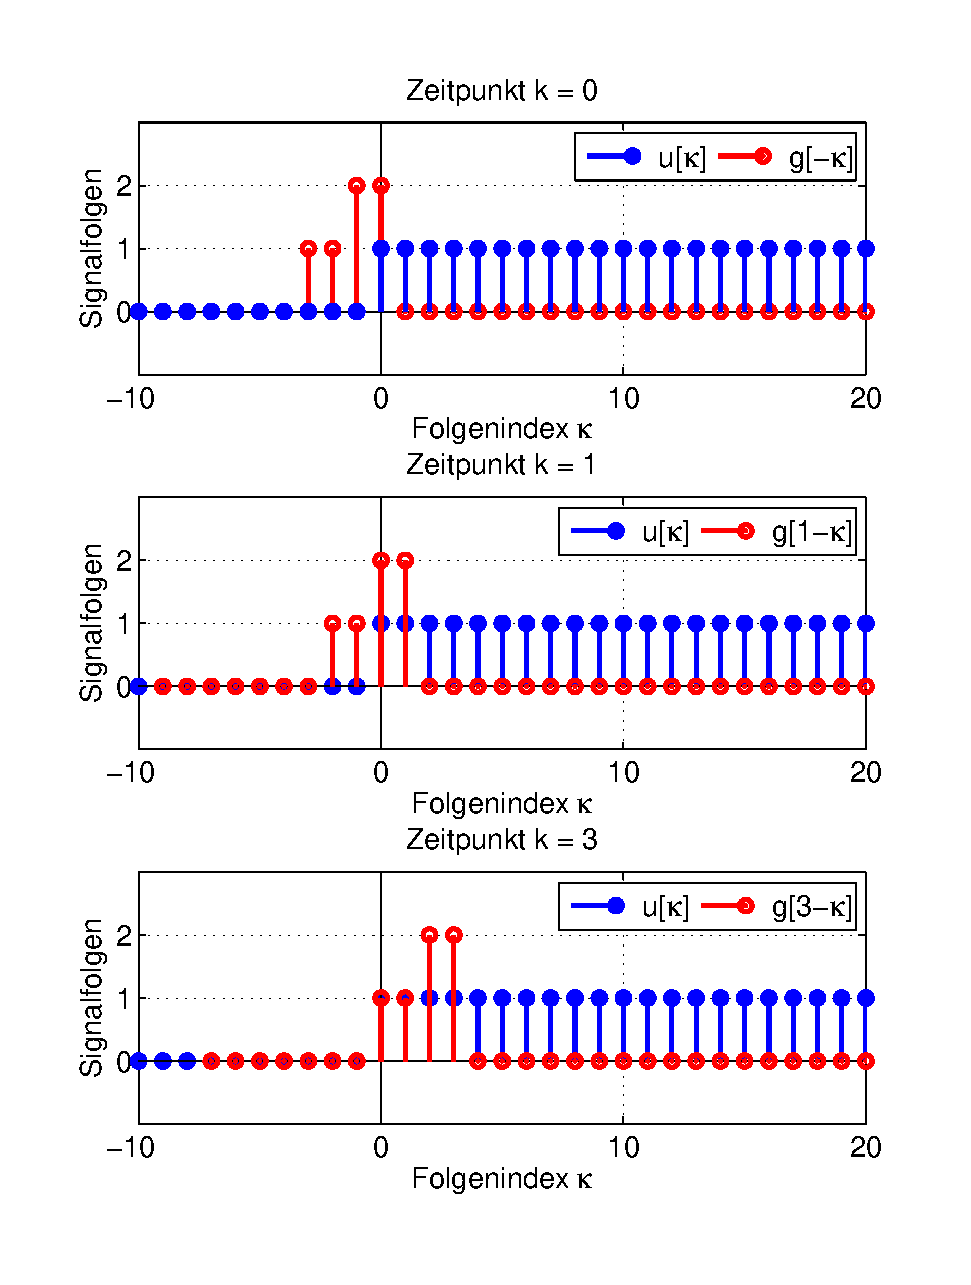
\includegraphics[width=0.5\textwidth]{Kapitel6/Bilder/image15.eps}}
  \caption{Pole und Nullstellen in der komplexen z-Ebene (Befehl pzmap)}
  \label{fig:SystemInterpretationMatlab}
\end{figure}

\noindent Dabei wird neben den Polen und Nullstellen gleich der Einheitskreis mit eingezeichnet, um die Stabilitätseigenschaften direkt ablesen zu können.

\noindent Die Impuls- und Sprungantworten werden mit dem Befehlen impulse(g,10) und step(g,10) dar-gestellt, wobei der Parameter 10 den größten Folgenindex festlegt.

\lstinputlisting[caption = {}]{Kapitel6/mat3.m}

\noindent MATLAB stellt die Ergebnisse als Stufenfunktion dar. Für das Beispiel ergeben sich die in Bild \ref{fig:SystemInterpretationMatlab1} dargestellten Signalverläufe.

\begin{figure}[H]
  \centerline{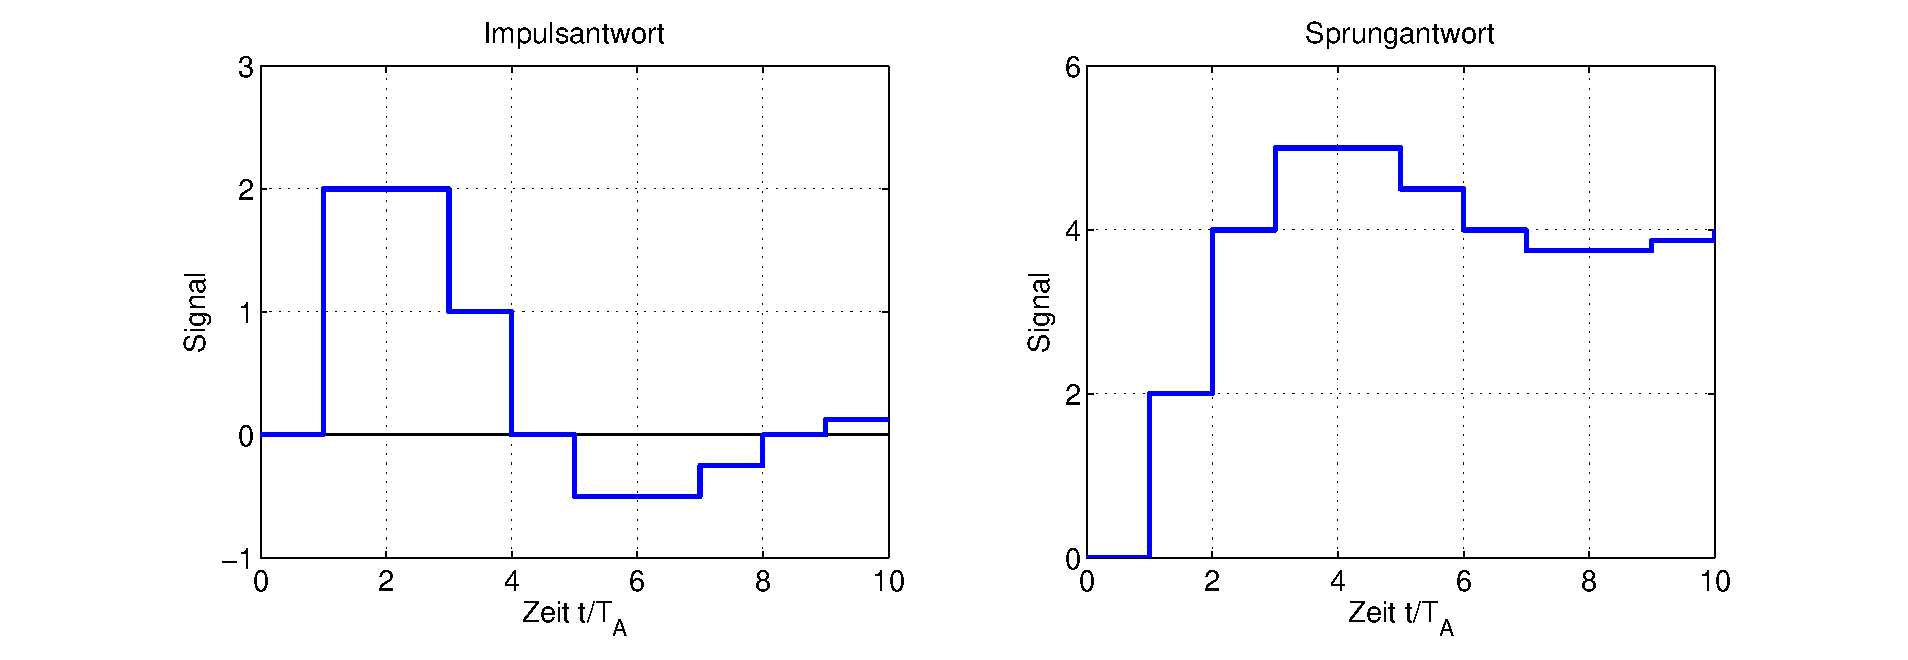
\includegraphics[width=1\textwidth]{Kapitel6/Bilder/image16.eps}}
  \caption{Impuls- und Sprungantwort berechnet mit MATLAB}
  \label{fig:SystemInterpretationMatlab1}
\end{figure}

\noindent Alternativ kann die Grafik unterdrückt und die Ergebnisse als Vektor abgespeichert werden. 

\lstinputlisting[caption = {}]{Kapitel6/mat4.m}

\noindent Weitere Informationen zu dem Verfahren können der MATLAB-Hilfe entnommen werden.

\subsubsection{Simulation eines zeitdiskreten Systems mit SIMULINK}

\noindent Neben der Berechnung von Systemantworten in MATLAB k\"{o}nnen Systeme als Blockschaltbilder in SIMULINK dargestellt werden. Dazu stellt SIMULINK verschiedene elementare \"{U}bertragungsglieder zur Verf\"{u}gung. Mit ihnen lassen sich Strukturen sehr detailliert darstellen oder als \"{U}bertragungsfunktionen implementieren.\bigskip

{\fontfamily{phv}\selectfont
\noindent\textbf{Signalquellen}}\smallskip

\noindent Mit Hilfe von Signalquellen werden Eingangssignale generiert. Neben den typischen Signalformen wie Sprung-, Rampen, Rechteck und Sinusfunktion erlaubt SIMULINK die Erzeugung von Signalquellen \"{u}ber selbst definierte Variablen oder sogenannte mat-Files. Damit ist es zum Beispiel auch m\"{o}glich, gemessene Daten als Signalquelle zu verwenden, indem die Messdaten als mat-File eingebunden werden. Tabelle \ref{tab:sixeight} stellt eine Auswahl von Signalquellen in SIMULINK dar.
\clearpage

\begin{table}[H]
\caption{Auswahl von Signalquellen in Simulink}
\setlength{\fboxsep}{0pt}%
\colorbox{lightgray}{%
\arrayrulecolor{white}%
\begin{tabular}{| c | c | c | c |}
\hline
\parbox[c][0.28in][c]{1.6in}{\smallskip\centering\textbf{\fontfamily{phv}\selectfont{Signalquelle}}} & \parbox[c][0.28in][c]{1.5in}{\smallskip\centering\textbf{\fontfamily{phv}\selectfont{Simulink Symbol}}} &
\parbox[c][0.28in][c]{1.6in}{\smallskip\centering\textbf{\fontfamily{phv}\selectfont{Signalquelle}}} &
\parbox[c][0.28in][c]{1.5in}{\smallskip\centering\textbf{\fontfamily{phv}\selectfont{Simulink Symbol}}}\\ \hline

\parbox[c][0.9in][c]{1.6in}{\centering{\fontfamily{phv}\selectfont{Konstante}}} &
\parbox[c][0.9in][c]{1.5in}{\centerline{\includegraphics[width=0.1\textwidth]{Kapitel6/Table1/image1.png}}} &
\parbox[c][0.9in][c]{1.6in}{\centering{\fontfamily{phv}\selectfont{Sinusfunktion}}} &
\parbox[c][0.9in][c]{1.5in}{\centerline{\includegraphics[width=0.1\textwidth]{Kapitel6/Table1/image2.png}}} \\ \hline

\parbox[c][0.9in][c]{1.6in}{\centering{\fontfamily{phv}\selectfont{Sprungfunktion}}} &
\parbox[c][0.9in][c]{1.5in}{\centerline{\includegraphics[width=0.085\textwidth]{Kapitel6/Table1/image3.png}}}&
\parbox[c][0.9in][c]{1.6in}{\centering{\fontfamily{phv}\selectfont{Zugriff auf Variable im Workspace}}} &
\parbox[c][0.9in][c]{1.5in}{\centerline{\includegraphics[width=0.12\textwidth]{Kapitel6/Table1/image4.png}}} \\ \hline

\parbox[c][0.9in][c]{1.6in}{\centering{\fontfamily{phv}\selectfont{Rampenfunktion}}} &
\parbox[c][0.9in][c]{1.5in}{\centerline{\includegraphics[width=0.085\textwidth]{Kapitel6/Table1/image5.png}}} &
\parbox[c][0.9in][c]{1.6in}{\centering{\fontfamily{phv}\selectfont{Definition in mat-File}}} &
\parbox[c][0.9in][c]{1.5in}{\centerline{\includegraphics[width=0.12\textwidth]{Kapitel6/Table1/image6.png}}} \\ \hline

\parbox[c][0.9in][c]{1.6in}{\centering{\fontfamily{phv}\selectfont{Rechteckfunktion}}} &
\parbox[c][0.9in][c]{1.5in}{\centerline{\includegraphics[width=0.1\textwidth]{Kapitel6/Table1/image7.png}}} &
\parbox[c][0.9in][c]{1.6in}{\centering{\fontfamily{phv}\selectfont{Zeit}}} &
\parbox[c][0.9in][c]{1.5in}{\centerline{\includegraphics[width=0.07\textwidth]{Kapitel6/Table1/image8.png}}}\\ \hline

\end{tabular}%
}\bigskip
\label{tab:sixten}
\end{table}

{\fontfamily{phv}\selectfont
\noindent\textbf{Signalpfade und Verknüpfung von Signalpfaden}}\smallskip

\noindent SIMULINK definiert Systeme über das Verbinden von Funktionsblöcken mit Signalpfaden. Zum Beispiel könnte ein System, das die Gleichung

\begin{equation}\label{eq:sixsonehundredtwentysix}
y\left[k\right]=3\cdot x\left[k\right]+5
\end{equation}

\noindent erf\"{u}llt, in SIMULINK \"{u}ber das Modell in Bild \ref{fig:DONTHAVE} dargestellt werden.

\begin{figure}[H]
  \centerline{\includegraphics[width=0.7\textwidth]{Kapitel6/Bilder/image17.png}}
  \caption{Einfaches SIMULINK Modell}
  \label{fig:DONTHAVE}
\end{figure}

\noindent Die Signalpfade laufen durch Bl\"{o}cke, die eine definierte Funktion ausf\"{u}hren. Diese Funktion kann neben Additionen, Subtraktion, Multiplikation und Division auch eine h\"{o}here mathematische Funktion sein, die als Math-Function-Block definiert wird. Mit den Bl\"{o}cken Multiplexer und Demultiplexer k\"{o}nnen Signale zu einem mehrdimensionalen Signalpfad zusammengefasst beziehungsweise von einem Signalpfad in einzelne Signale zerlegt werden. Tabelle \ref{tab:sixnine} stellt eine Auswahl von Verkn\"{u}pfungen in SIMULINK dar.

\clearpage

\begin{table}[H]
\caption{Auswahl von Funktionen zur Signalverknüpfung}
\setlength{\fboxsep}{0pt}%
\colorbox{lightgray}{%
\arrayrulecolor{white}%
\begin{tabular}{| c | c | c | c |}
\hline
\parbox[c][0.28in][c]{1.6in}{\smallskip\centering\textbf{\fontfamily{phv}\selectfont{Operation}}} & \parbox[c][0.28in][c]{1.5in}{\smallskip\centering\textbf{\fontfamily{phv}\selectfont{Simulink Symbol}}} &
\parbox[c][0.28in][c]{1.6in}{\smallskip\centering\textbf{\fontfamily{phv}\selectfont{Operation}}} &
\parbox[c][0.28in][c]{1.5in}{\smallskip\centering\textbf{\fontfamily{phv}\selectfont{Simulink Symbol}}}\\ \hline


\parbox[c][0.9in][c]{1.6in}{\centering{\fontfamily{phv}\selectfont{Addition von Signalen}}} &
\parbox[c][0.9in][c]{1.5in}{\centerline{\includegraphics[width=0.1\textwidth]{Kapitel6/Table1/image9.png}}} &
\parbox[c][0.9in][c]{1.6in}{\centering{\fontfamily{phv}\selectfont{Multiplikation / Division \\ von Signalen}}} &
\parbox[c][0.9in][c]{1.5in}{\centerline{\includegraphics[width=0.1\textwidth]{Kapitel6/Table1/image10.png}}} \\ \hline

\parbox[c][0.9in][c]{1.6in}{\centering{\fontfamily{phv}\selectfont{Multiplikation \\
mit einem Faktor, \\
Verstärkung}}} &
\parbox[c][0.9in][c]{1.5in}{\centerline{\includegraphics[width=0.1\textwidth]{Kapitel6/Table1/image11.png}}} &
\parbox[c][0.9in][c]{1.6in}{\centering{\fontfamily{phv}\selectfont{Mathematische \\
Funktionen}}} &
\parbox[c][0.9in][c]{1.5in}{\centerline{\includegraphics[width=0.1\textwidth]{Kapitel6/Table1/image12.png}}} \\ \hline

\parbox[c][0.9in][c]{1.6in}{\centering{\fontfamily{phv}\selectfont{Multiplexer}}} &
\parbox[c][0.9in][c]{1.5in}{\centerline{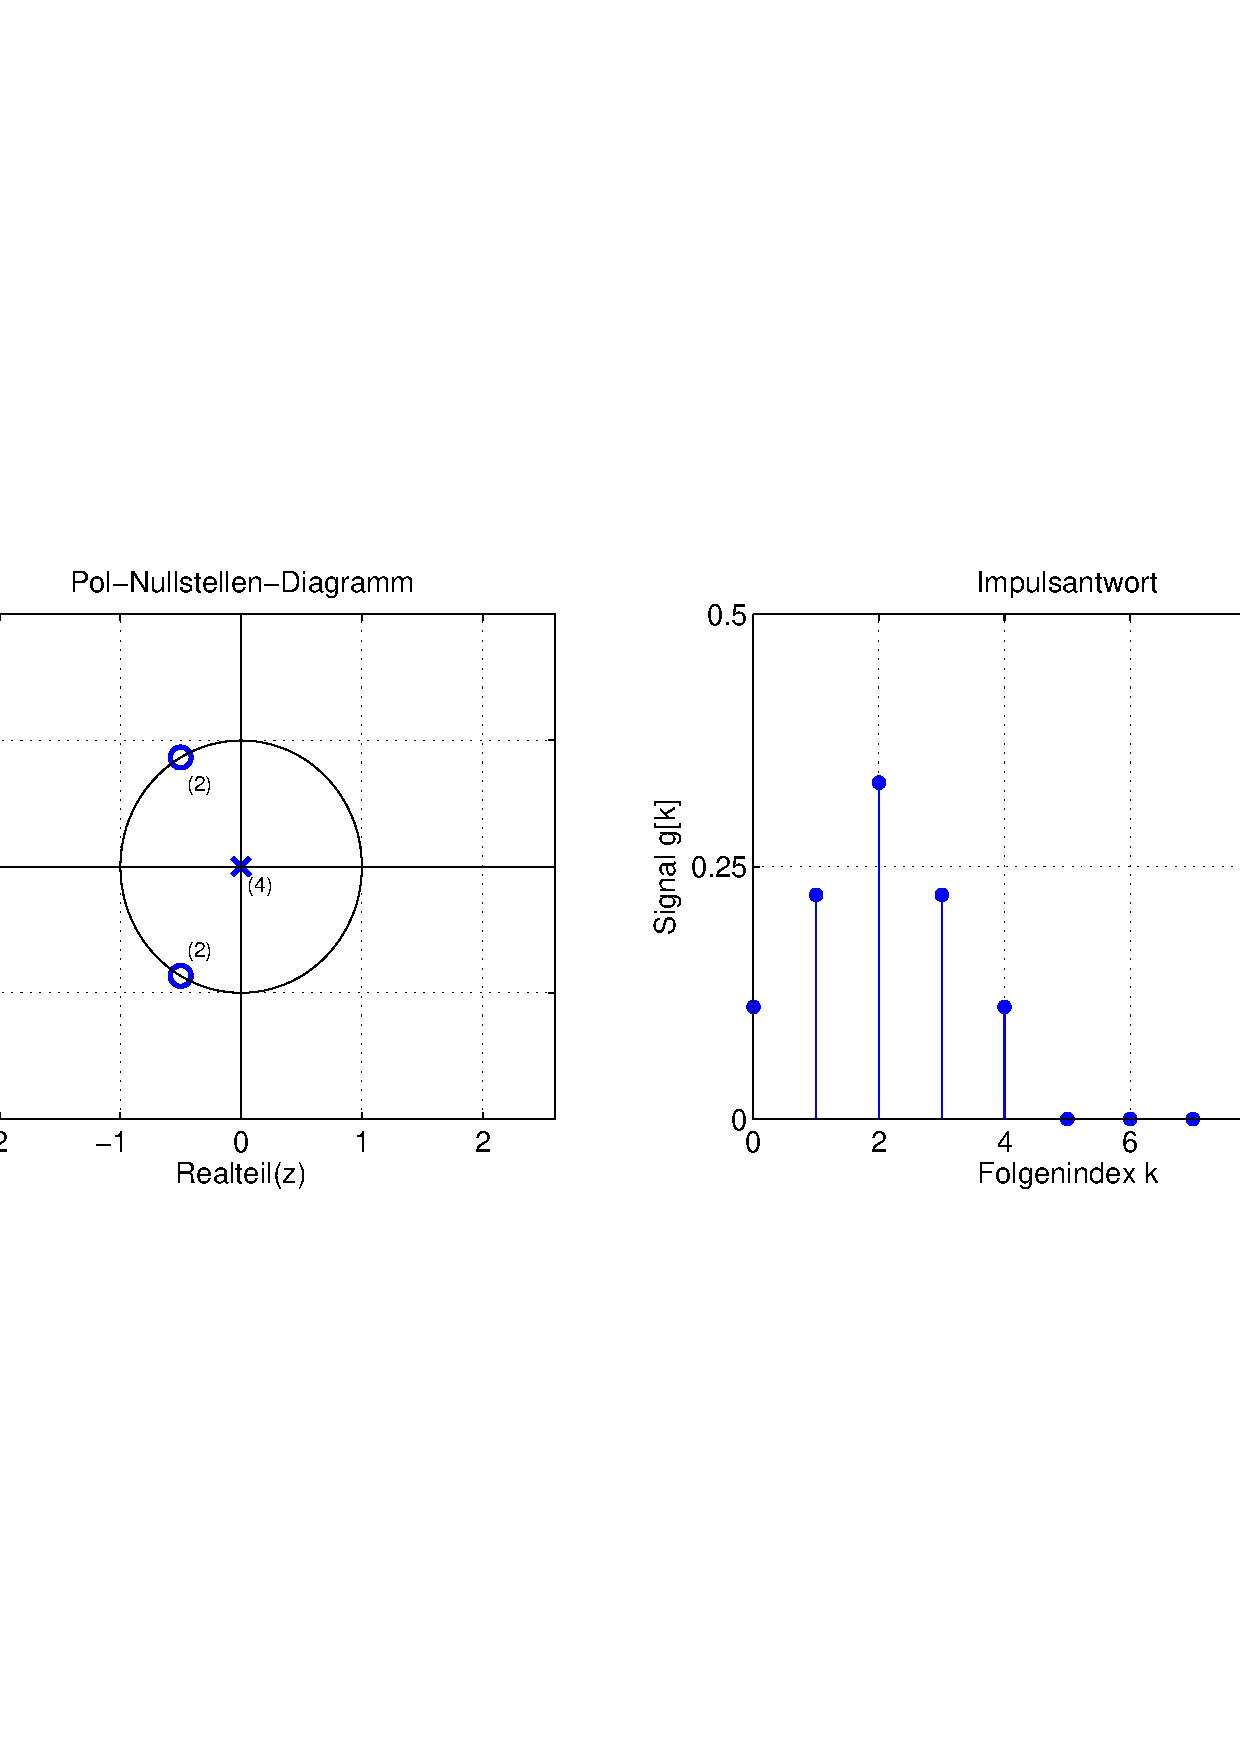
\includegraphics[width=0.05\textwidth]{Kapitel6/Table1/image13.png}}} &
\parbox[c][0.9in][c]{1.6in}{\centering{\fontfamily{phv}\selectfont{Demultiplexer}}} &
\parbox[c][0.9in][c]{1.5in}{\centerline{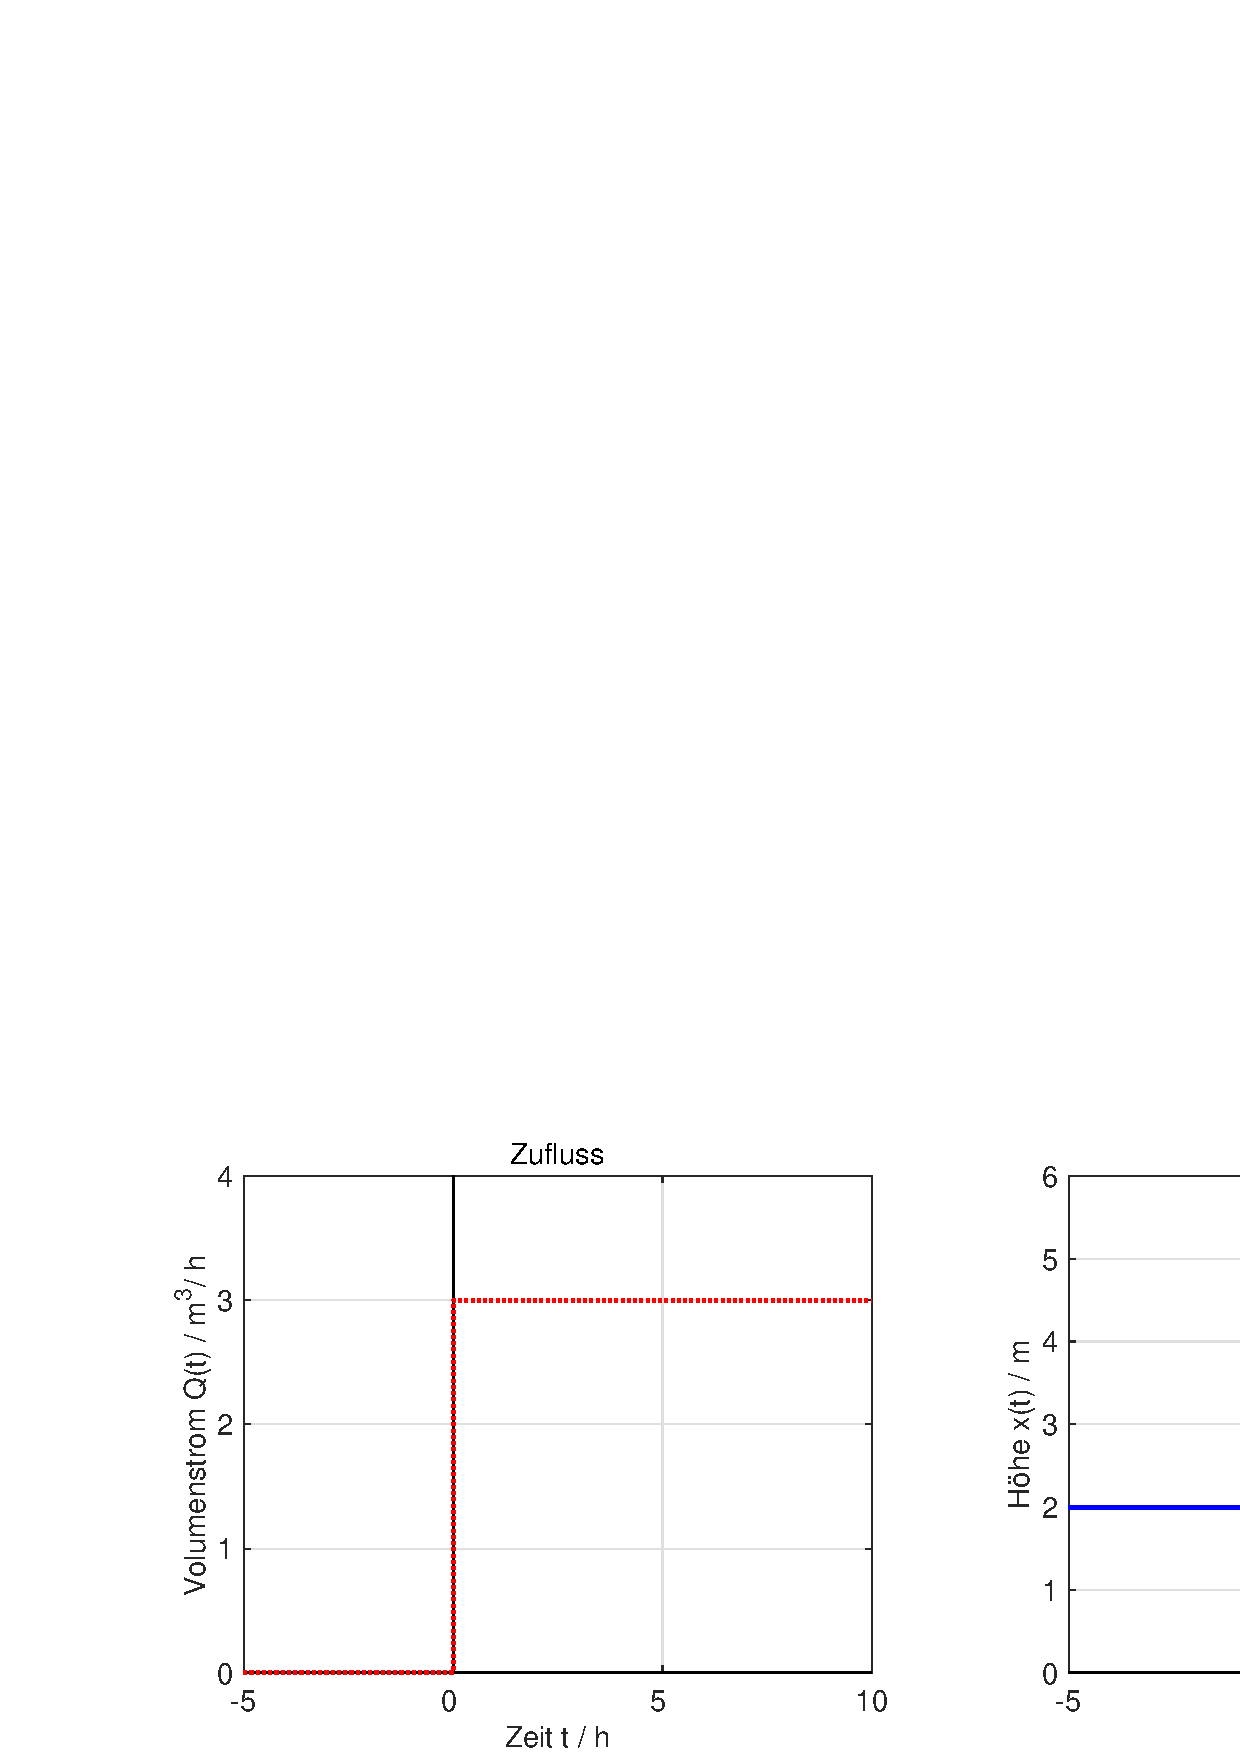
\includegraphics[width=0.05\textwidth]{Kapitel6/Table1/image14.png}}} \\ \hline 

\end{tabular}%
}\bigskip
\label{tab:sixeleven}
\end{table}

{\fontfamily{phv}\selectfont
\noindent\textbf{Elementare \"{U}bertragungsglieder}}\smallskip

\noindent Neben fest definierten \"{U}bertragungsgliedern wie Verz\"{o}gerung, Ableitung oder Integral bietet SIMULINK die M\"{o}glichkeit, \"{U}bertragungsglieder \"{u}ber ihre z-Transformierte selbst zu definieren. Die \"{U}bertragungsglieder k\"{o}nnen als gebrochen rationale Funktion oder in Linearfaktor-Schreibweise definiert werden. Tabelle \ref{tab:sixten} zeigt eine Auswahl von Funktionsbl\"{o}cken f\"{u}r zeitdiskrete \"{U}bertragungsfunktionen in SIMULINK.

\begin{table}[H]
\caption{Auswahl von Funktionen zur Signalverknüpfung}
\setlength{\fboxsep}{0pt}%
\colorbox{lightgray}{%
\arrayrulecolor{white}%
\begin{tabular}{| c | c | c | c |}
\hline
\parbox[c][0.28in][c]{1.6in}{\smallskip\centering\textbf{\fontfamily{phv}\selectfont{Operation}}} & \parbox[c][0.28in][c]{1.5in}{\smallskip\centering\textbf{\fontfamily{phv}\selectfont{Simulink Symbol}}} &
\parbox[c][0.28in][c]{1.6in}{\smallskip\centering\textbf{\fontfamily{phv}\selectfont{Operation}}} &
\parbox[c][0.28in][c]{1.5in}{\smallskip\centering\textbf{\fontfamily{phv}\selectfont{Simulink Symbol}}}\\ \hline


\parbox[c][0.9in][c]{1.6in}{\centering{\fontfamily{phv}\selectfont{Verzögerung}}} &
\parbox[c][0.9in][c]{1.5in}{\centerline{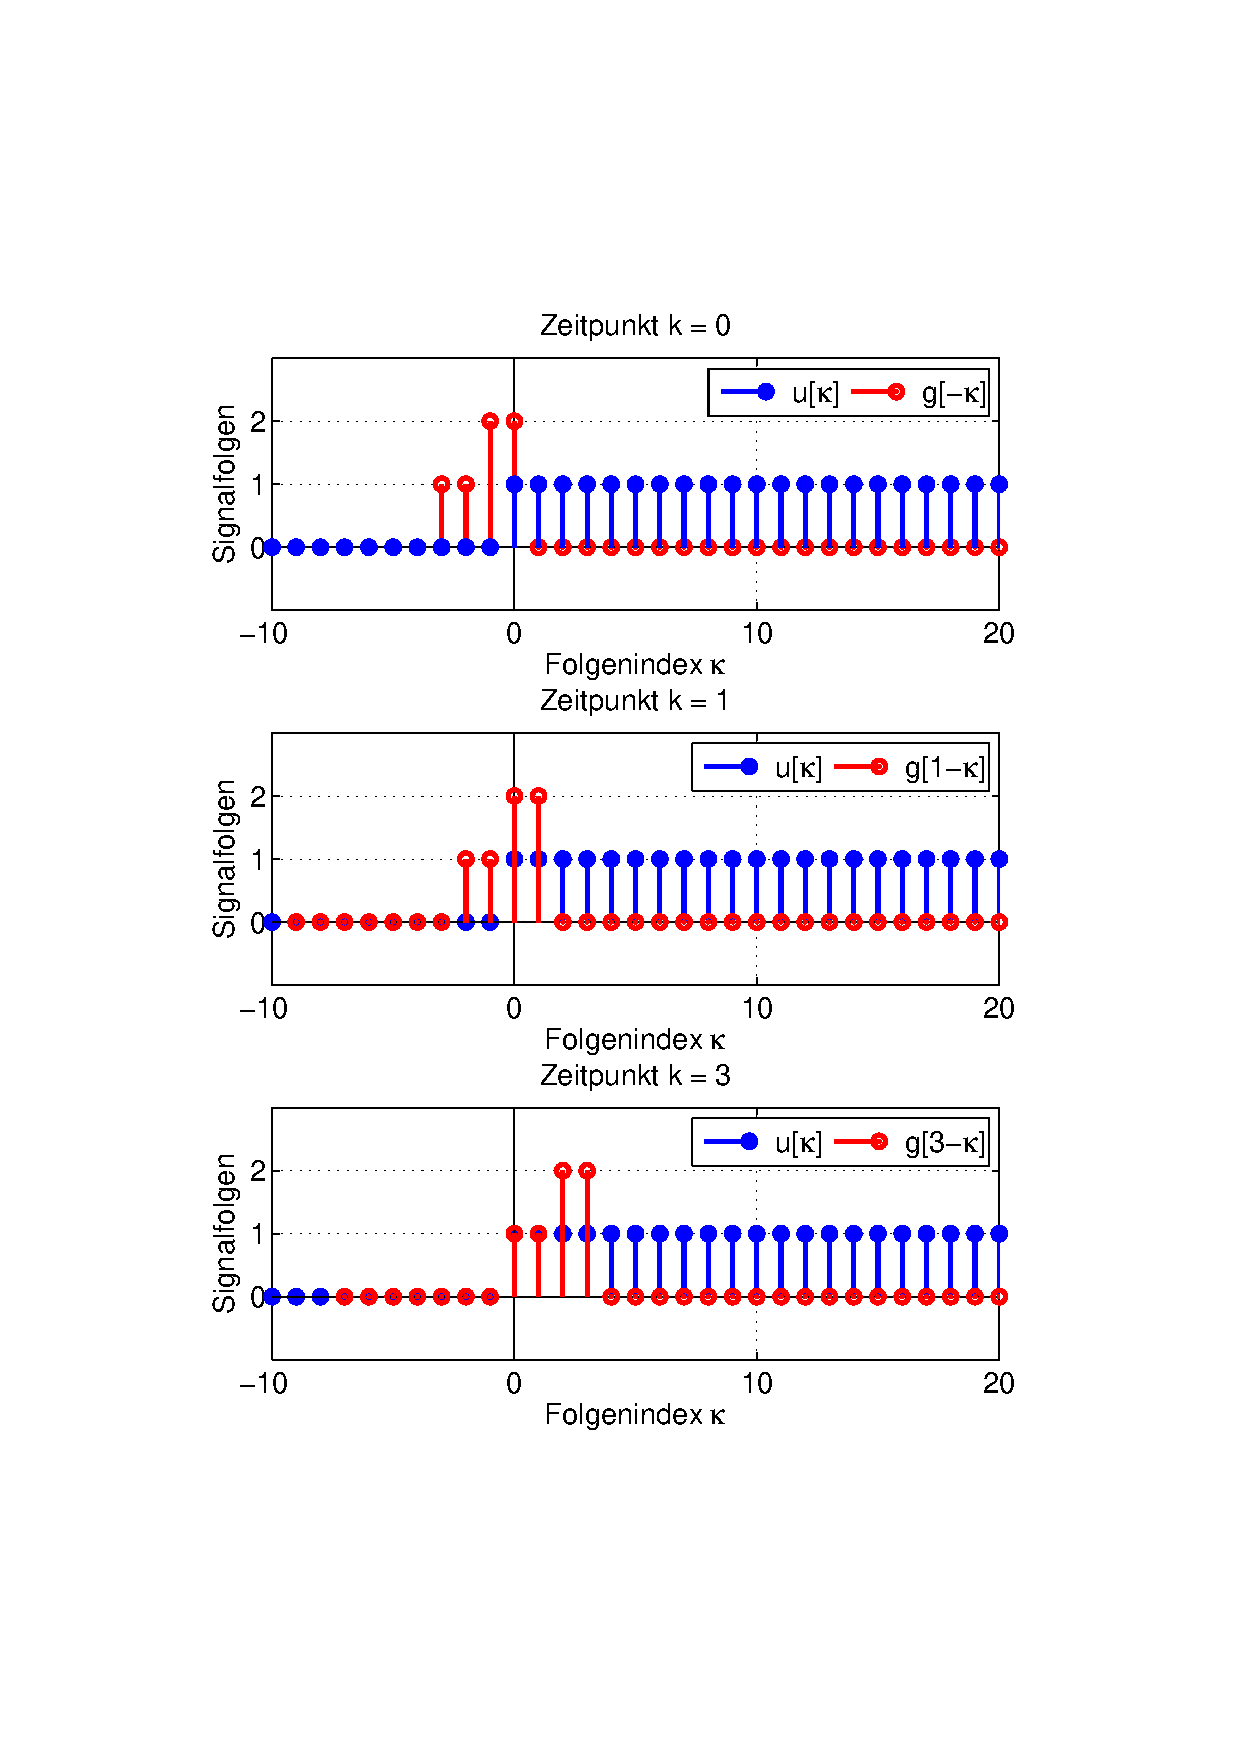
\includegraphics[width=0.1\textwidth]{Kapitel6/Table1/image15.png}}} &
\parbox[c][0.9in][c]{1.6in}{\centering{\fontfamily{phv}\selectfont{Pol-Nullstellen \\
Übertragungsfunktion}}} &
\parbox[c][0.9in][c]{1.5in}{\centerline{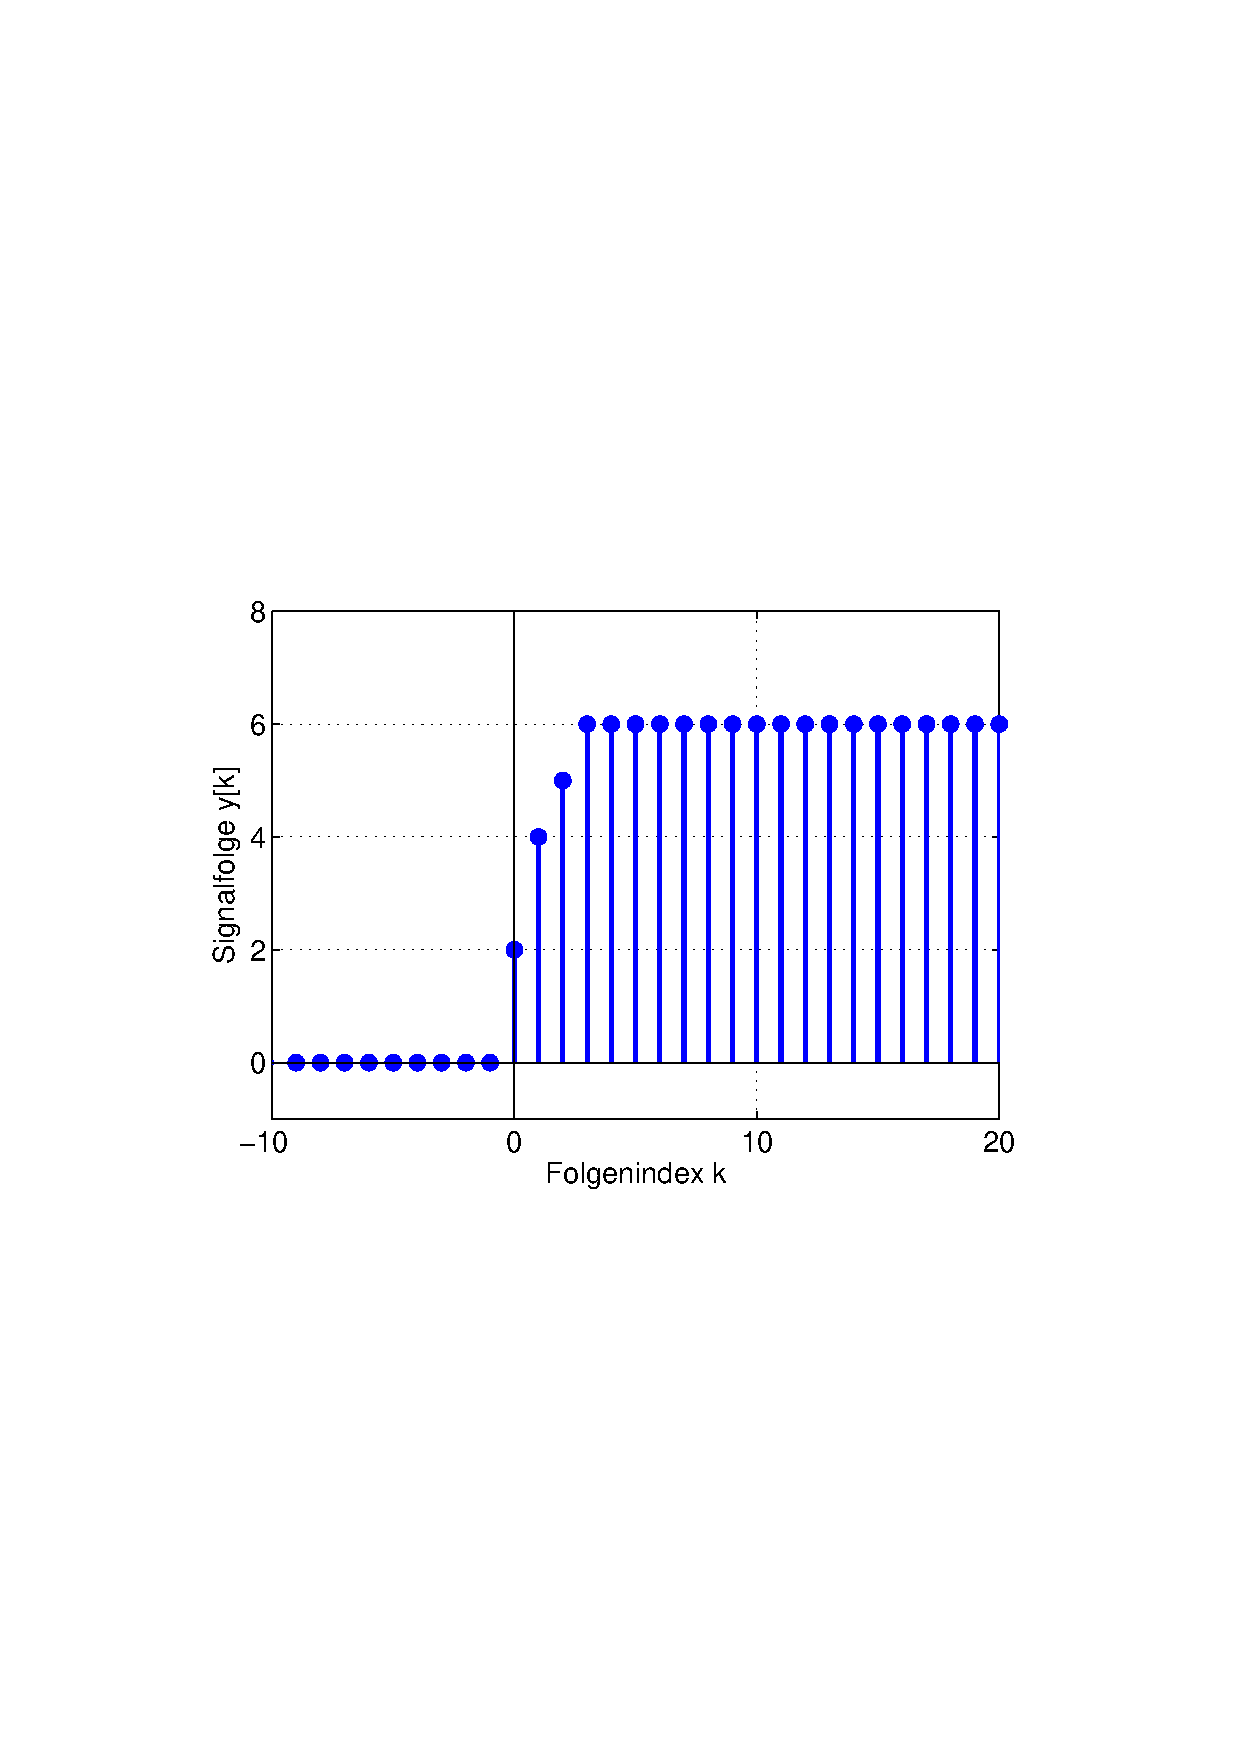
\includegraphics[width=0.13\textwidth]{Kapitel6/Table1/image16.png}}} \\ \hline

\parbox[c][0.9in][c]{1.6in}{\centering{\fontfamily{phv}\selectfont{Ableitung}}} &
\parbox[c][0.9in][c]{1.5in}{\centerline{\includegraphics[width=0.15\textwidth]{Kapitel6/Table1/image17.png}}} &
\parbox[c][0.9in][c]{1.6in}{\centering{\fontfamily{phv}\selectfont{Gebrochen rationale  \\
Übertragungsfunktion}}} &
\parbox[c][0.9in][c]{1.5in}{\centerline{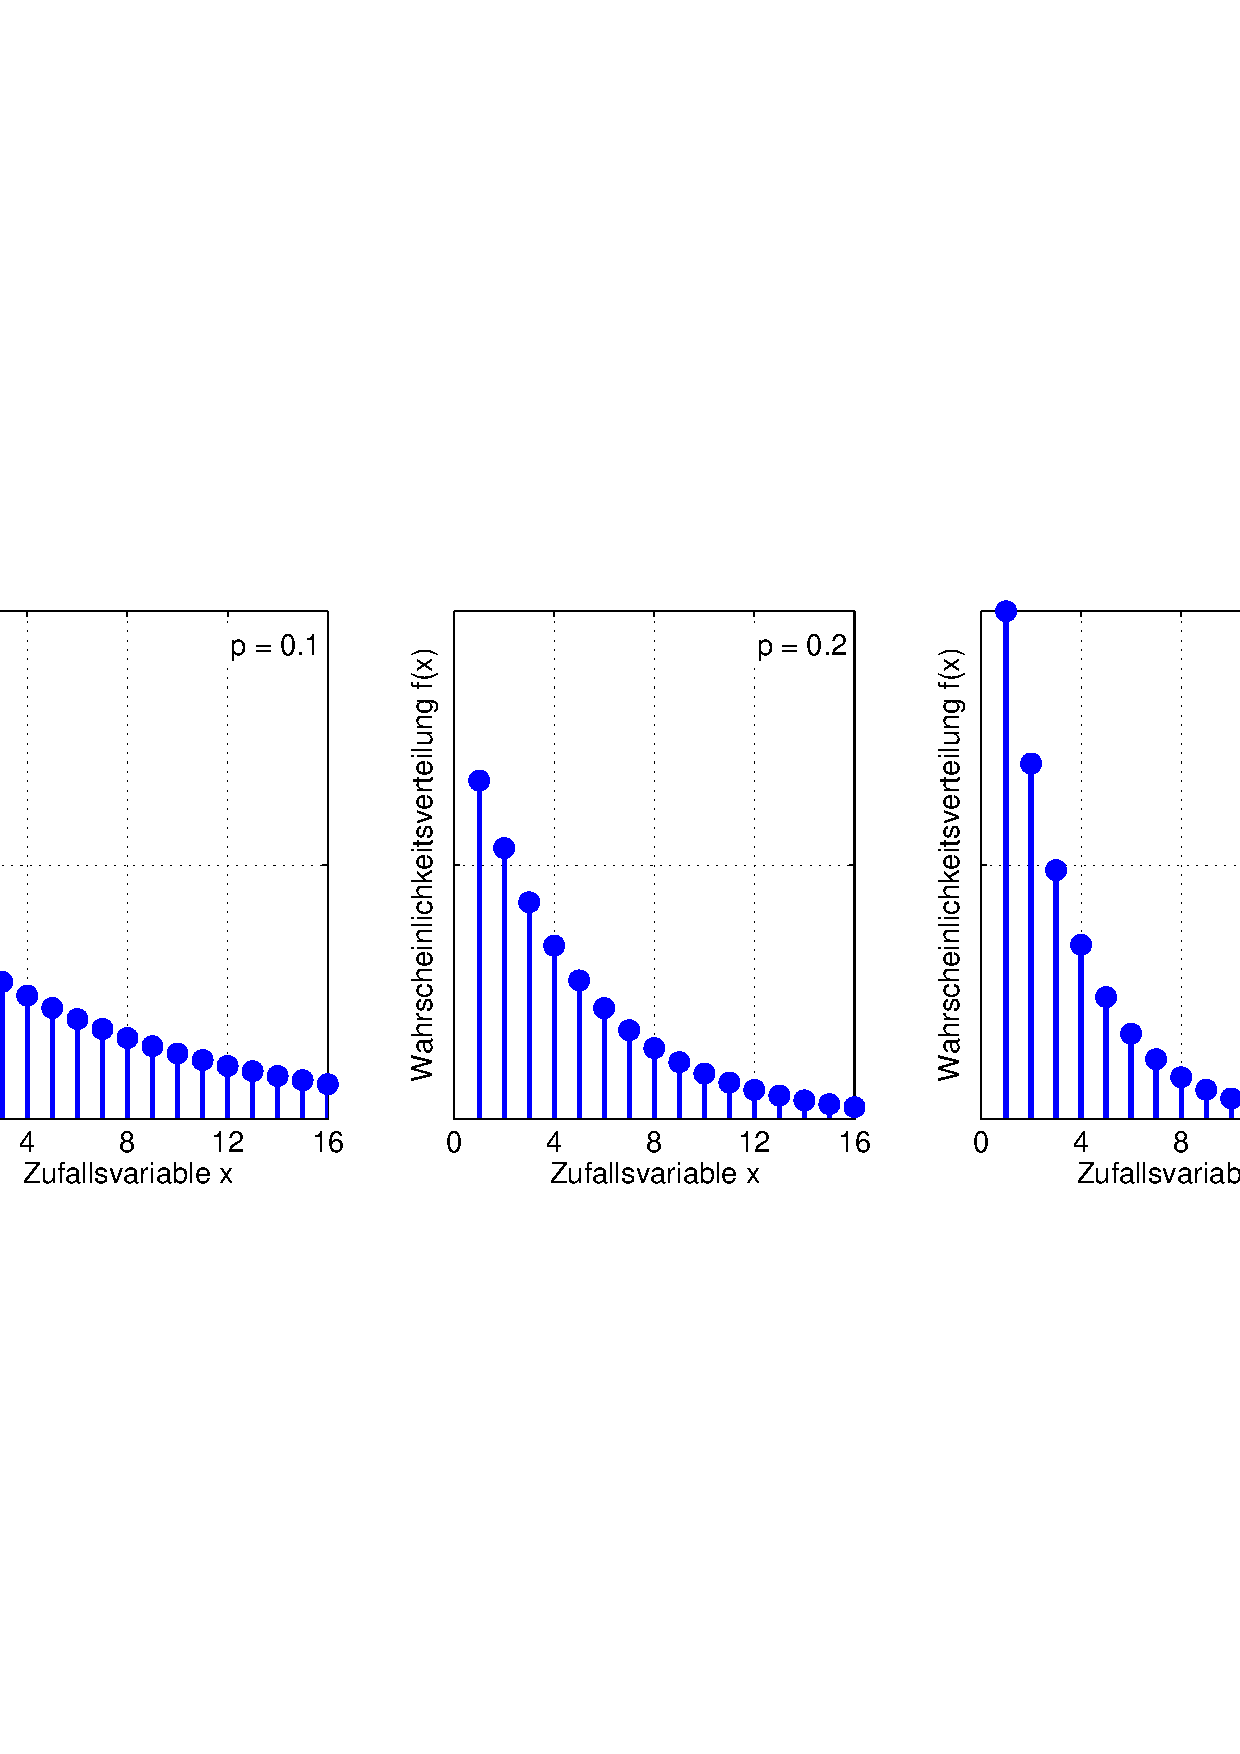
\includegraphics[width=0.12\textwidth]{Kapitel6/Table1/image18.png}}} \\ \hline

\parbox[c][0.9in][c]{1.6in}{\centering{\fontfamily{phv}\selectfont{Integral}}} &
\parbox[c][0.9in][c]{1.5in}{\centerline{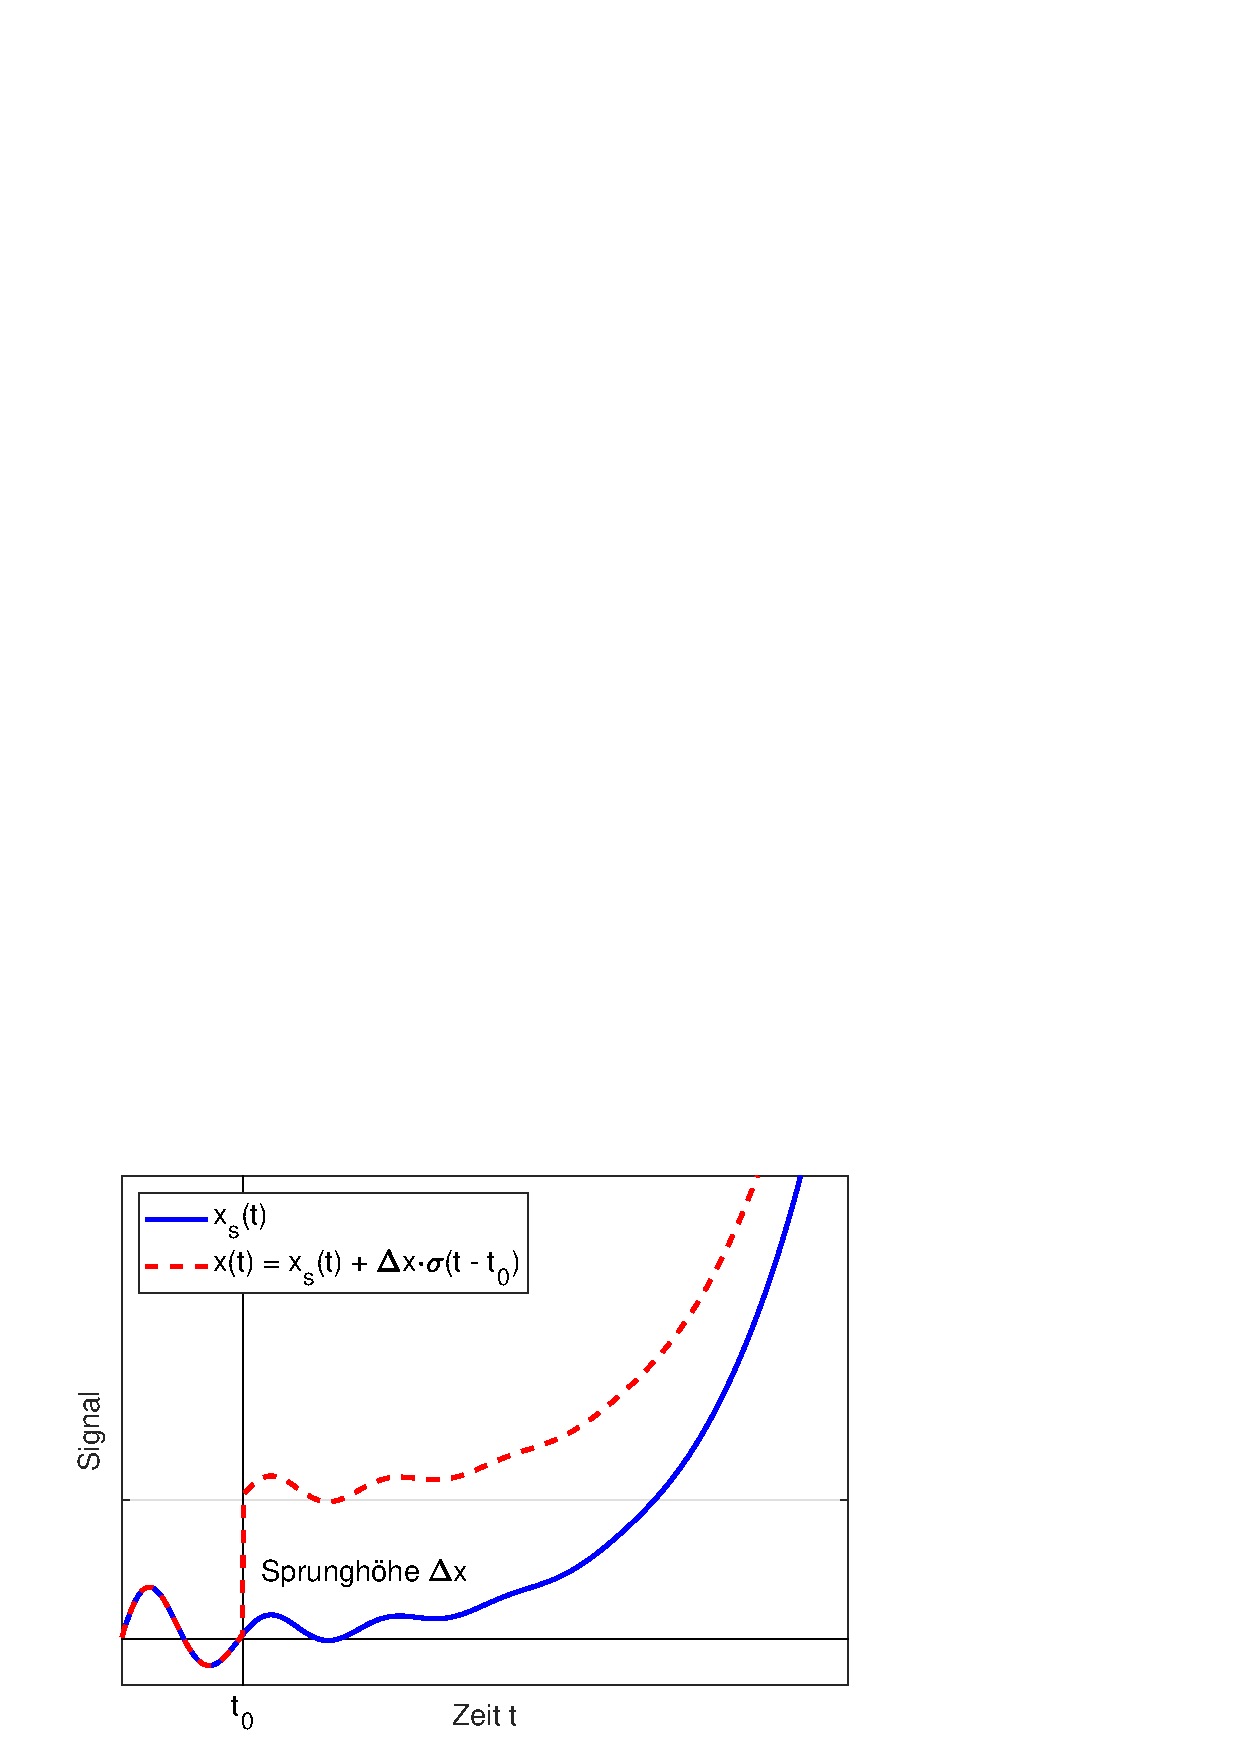
\includegraphics[width=0.12\textwidth]{Kapitel6/Table1/image19.png}}} &
\parbox[c][0.9in][c]{1.6in}{\centering{\fontfamily{phv}\selectfont{Gewichteter \\
Mittelwert}}} &
\parbox[c][0.9in][c]{1.5in}{\centerline{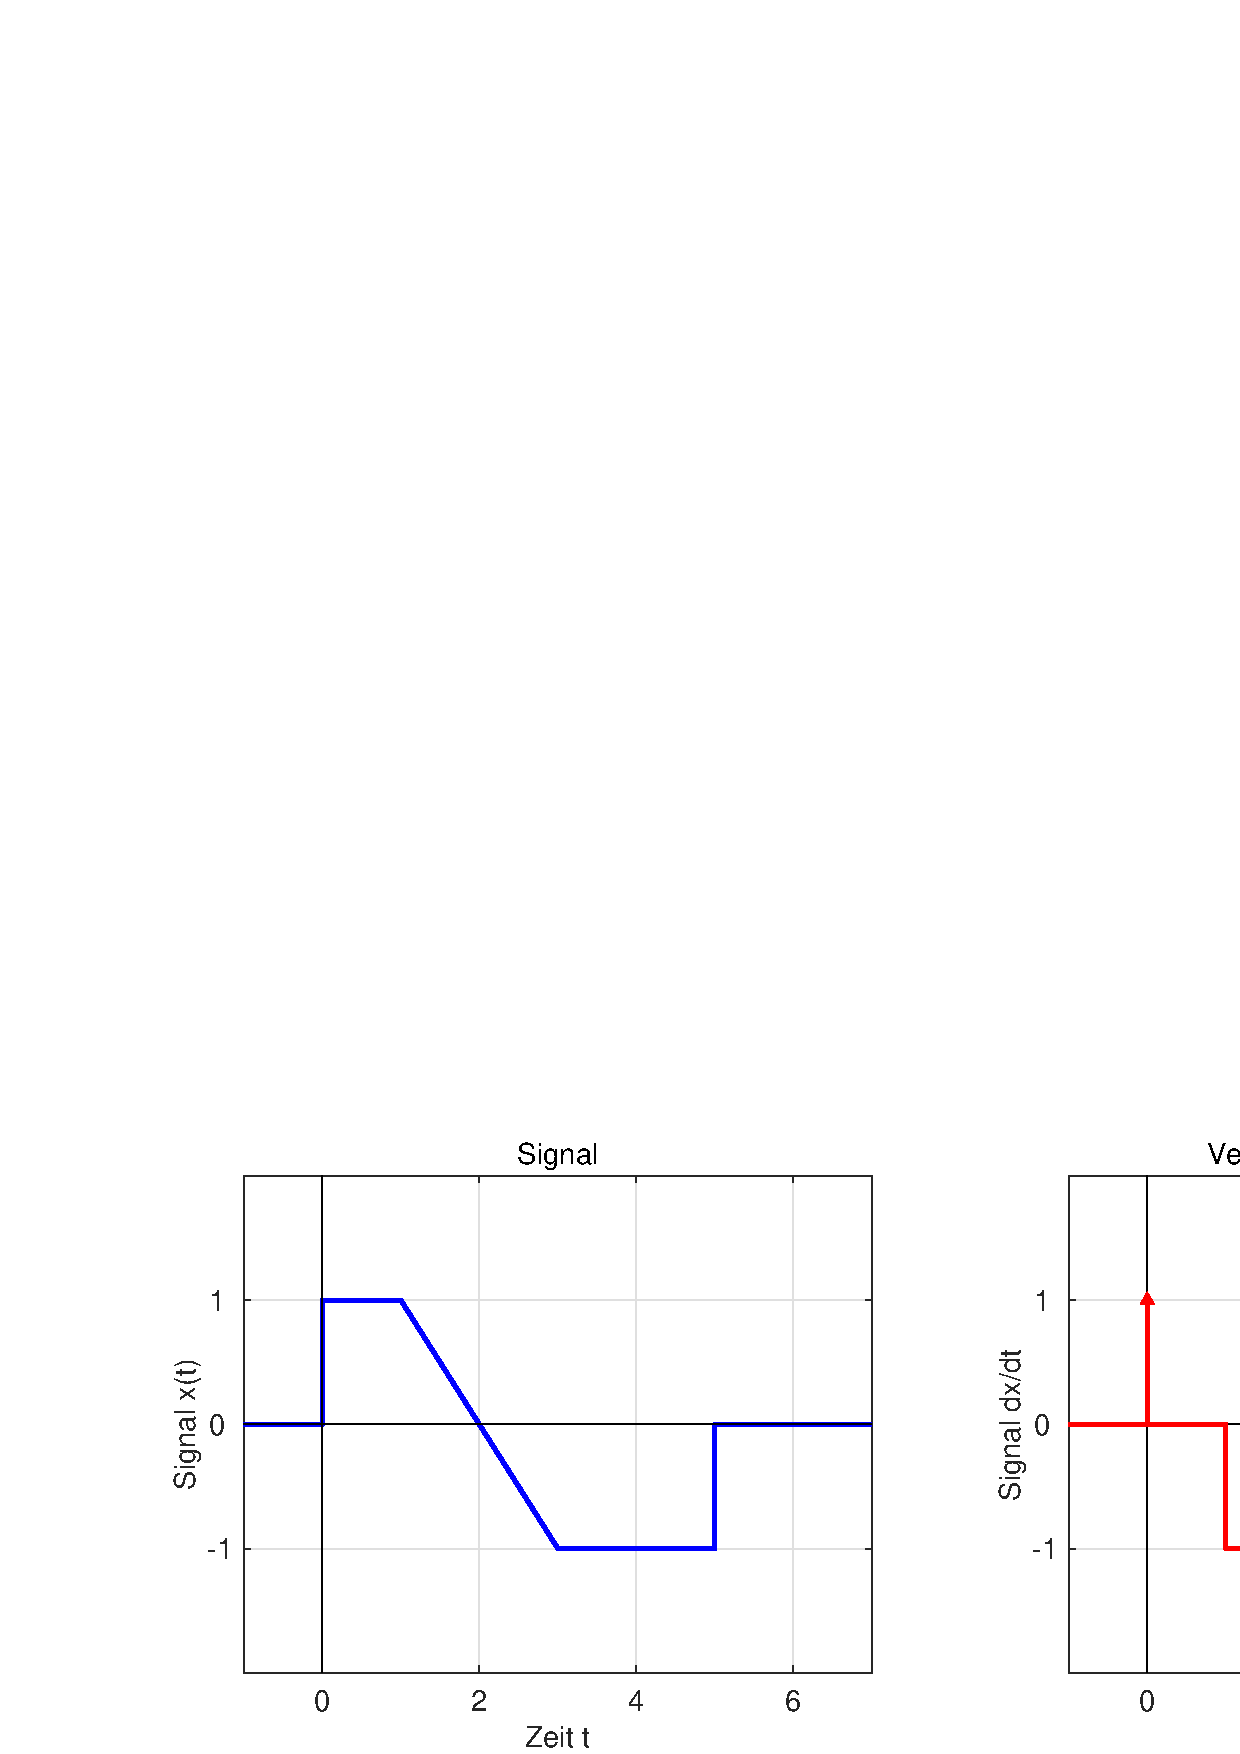
\includegraphics[width=0.19\textwidth]{Kapitel6/Table1/image20.png}}} \\ \hline 

\parbox[c][0.9in][c]{1.6in}{\centering{\fontfamily{phv}\selectfont{Zero-Order-Hold}}} &
\parbox[c][0.9in][c]{1.5in}{\centerline{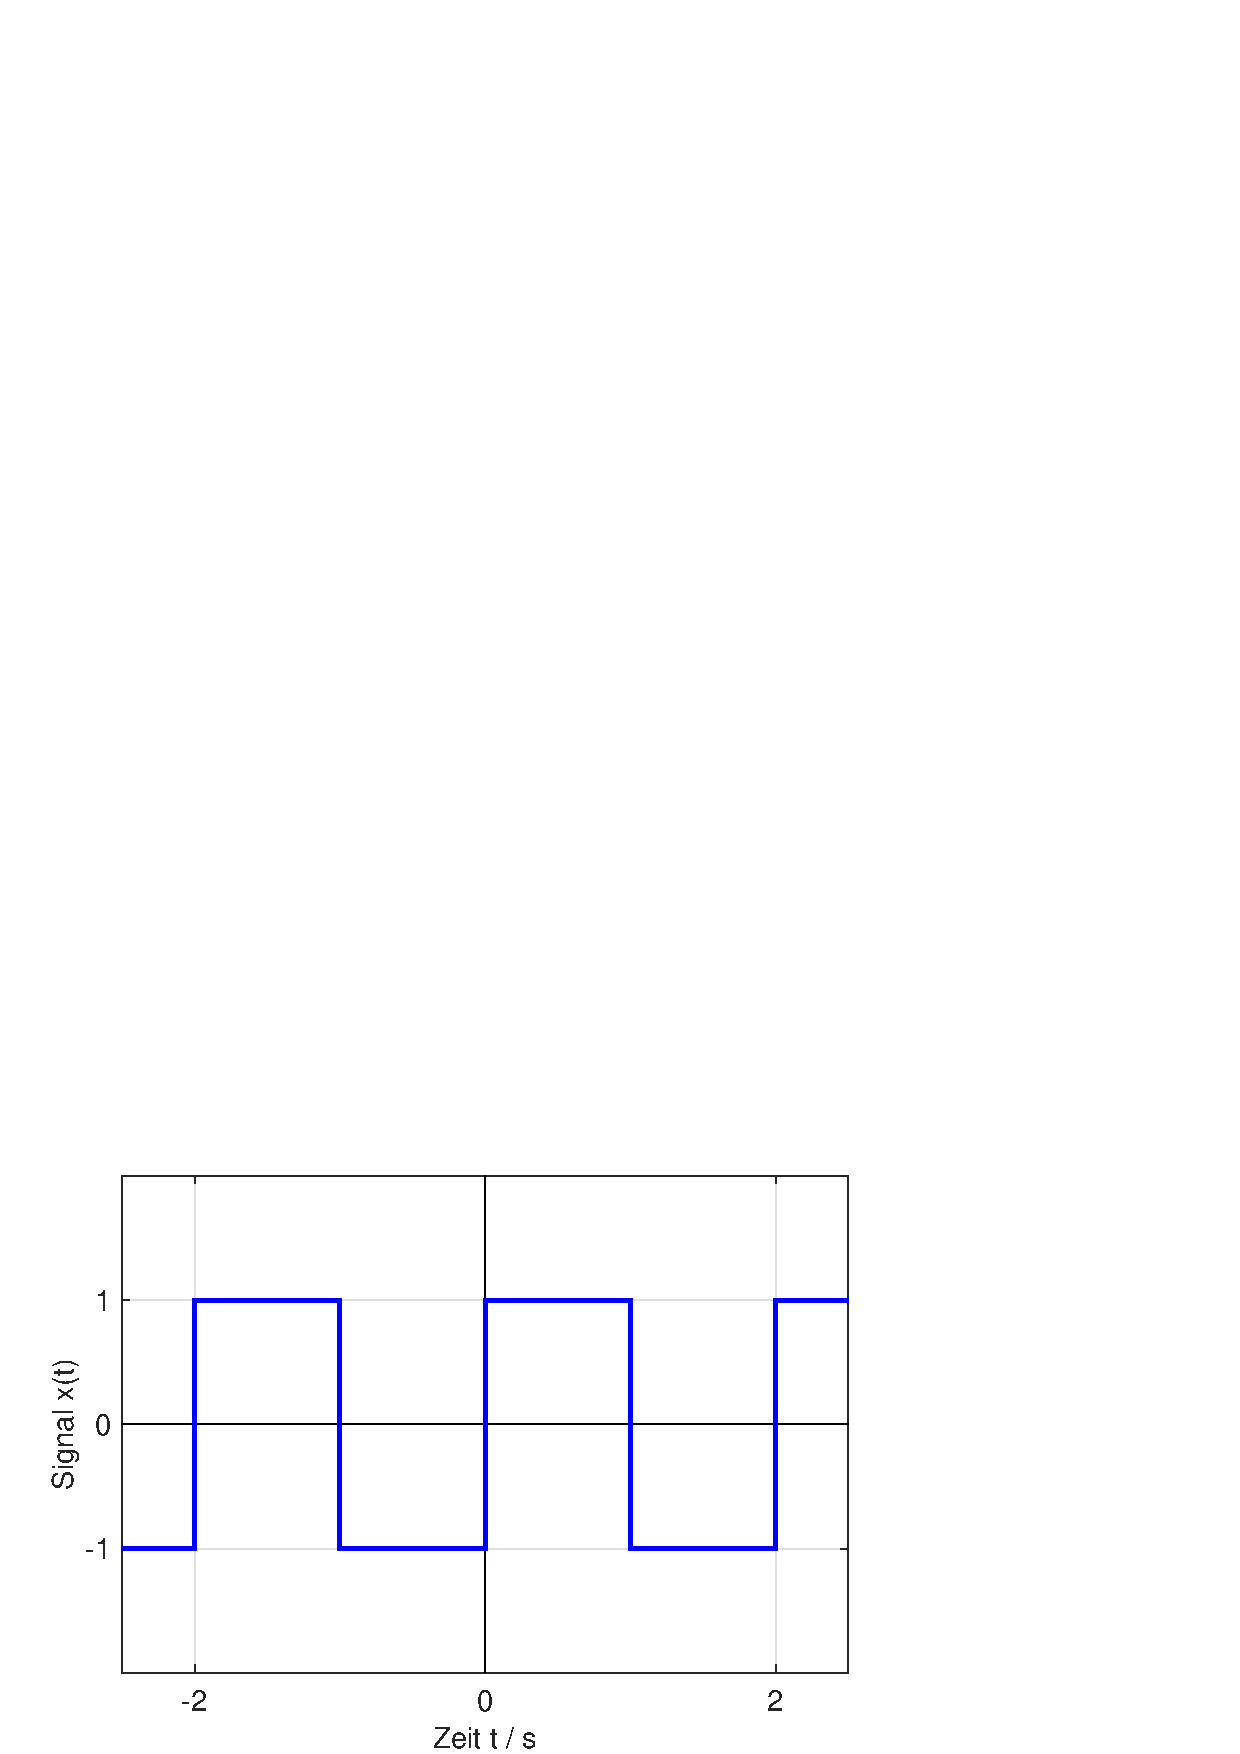
\includegraphics[width=0.1\textwidth]{Kapitel6/Table1/image21.png}}} &
\parbox[c][0.9in][c]{1.6in}{\centering{\fontfamily{phv}\selectfont{First-Order-Hold}}} &
\parbox[c][0.9in][c]{1.5in}{\centerline{\includegraphics[width=0.1\textwidth]{Kapitel6/Table1/image22.png}}} \\ \hline 

\end{tabular}%
}\bigskip
\label{tab:sixtwelve}
\end{table}

{\fontfamily{phv}\selectfont
\noindent\textbf{Signalsenken}}\smallskip

\noindent Die in SIMULINK berechneten Signalpfade enden in sogenannten Signalsenken. Signalsenken stellen das Signal grafisch dar oder speichern das Signal in Variablen oder mat-Files. Tabelle \ref{tab:sixeleven} stellt eine Auswahl von Signalquellen in SIMULINK dar.

\begin{table}[H]
\caption{Auswahl von Funktionen zur Signalverknüpfung}
\setlength{\fboxsep}{0pt}%
\colorbox{lightgray}{%
\arrayrulecolor{white}%
\begin{tabular}{| c | c | c | c |}
\hline
\parbox[c][0.28in][c]{1.6in}{\smallskip\centering\textbf{\fontfamily{phv}\selectfont{Operation}}} & \parbox[c][0.28in][c]{1.5in}{\smallskip\centering\textbf{\fontfamily{phv}\selectfont{Simulink Symbol}}} &
\parbox[c][0.28in][c]{1.6in}{\smallskip\centering\textbf{\fontfamily{phv}\selectfont{Operation}}} &
\parbox[c][0.28in][c]{1.5in}{\smallskip\centering\textbf{\fontfamily{phv}\selectfont{Simulink Symbol}}}\\ \hline

\parbox[c][0.9in][c]{1.6in}{\centering{\fontfamily{phv}\selectfont{Numerische \\
Anzeige}}} &
\parbox[c][0.9in][c]{1.5in}{\centerline{\includegraphics[width=0.19\textwidth]{Kapitel6/Table1/image23.png}}} &
\parbox[c][0.9in][c]{1.6in}{\centering{\fontfamily{phv}\selectfont{Grafische \\
Darstellung}}} &
\parbox[c][0.9in][c]{1.5in}{\centerline{\includegraphics[width=0.1\textwidth]{Kapitel6/Table1/image24.png}}} \\ \hline

\parbox[c][0.9in][c]{1.6in}{\centering{\fontfamily{phv}\selectfont{Speicherung in \\
Ausgangsvariable}}} &
\parbox[c][0.9in][c]{1.5in}{\centerline{\includegraphics[width=0.15\textwidth]{Kapitel6/Table1/image25.png}}} &
\parbox[c][0.9in][c]{1.6in}{\centering{\fontfamily{phv}\selectfont{Speicherung \\
in mat-File}}} &
\parbox[c][0.9in][c]{1.5in}{\centerline{\includegraphics[width=0.15\textwidth]{Kapitel6/Table1/image26.png}}} \\ \hline

\end{tabular}%
}\bigskip
\label{tab:sixthirteen}
\end{table}

{\fontfamily{phv}\selectfont
\noindent\textbf{Simulationsvarianten zeitdiskreter Systeme}}\smallskip

\noindent Zeitdiskrete Systeme k\"{o}nnen auf zweierlei Arten simuliert werden:

\begin{itemize}
    \item Fixed-Step-Simulation
    \item Variable-Step-Simulation
\end{itemize}

\noindent Bei der Fixed-Step-Simulation des Systems wird bei den Solver Optionen ein Fixed-Step-Solver-Typ mit dem Solver discrete (no continuous states) verwendet. Die Simulation wird damit in zeitlich konstanten Schritten durchgef\"{u}hrt, die der Abtastzeit entsprechen. Dieser Simulationstyp eignet sich f\"{u}r rein digitale Simulationen. 

\begin{figure}[H]
  \centerline{\includegraphics[width=0.7\textwidth]{Kapitel6/Bilder/image18.png}}
  \caption{Konfiguration in SIMULINK für eine Fixed-Step-Simulation}
  \label{fig:DONTHAVE2}
\end{figure}

\noindent Alternativ kann zu der Fixed-Step-Simulation eine Simulation mit variabler Schrittweite durchgef\"{u}hrt werden. Die zeitliche Diskretisierung des Signals erfolgt in diesem Fall mit einem Halteglied (Zero-Order-Hold), das das Eingangssignal f\"{u}r eine Periodendauer festh\"{a}lt. Der Vorteil dieser Simulationsart ist, dass die Werte, die sich aus der digitalen Signalerarbeitung ergeben, analog weiterverarbeitet werden k\"{o}nnen. Zum Beispiel kann eine analoge Tiefpass-Filterung durchgef\"{u}hrt werden. \bigskip

\noindent
\colorbox{lightgray}{%
\arrayrulecolor{white}%
\renewcommand\arraystretch{0.6}%
\begin{tabular}{ wl{16.5cm} }
{\fontfamily{phv}\selectfont{Beispiel: Vergleich einer zeitkontinuierlichen und zeitdiskreten Simulation}}
\end{tabular}%
}\medskip

\noindent Zur Verdeutlichung der beiden Simulationsarten wird das System mit der \"{U}bertragungsfunktion 

\begin{equation}\label{eq:sixsonehundredtwentyseven}
G\left(z\right)=\frac{2\cdot z}{z^{2} -z+0.5}
\end{equation}

\noindent einmal mit konstanter Schrittweite (Bild \ref{fig:SimModel1}) und einmal zeitkontinuierlich mit Halteglied (Bild \ref{fig:SimModel2}) simuliert. Das digitale Signal wird anschlie{\ss}end mit einem analogen Tiefpass gefiltert.

\begin{figure}[H]
  \centerline{\includegraphics[width=1\textwidth]{Kapitel6/Bilder/image19.png}}
  \caption{SIMULINK-Modell f\"{u}r eine Fixed-Step-Simulation}
  \label{fig:SimModel1}
\end{figure}


\begin{figure}[H]
  \centerline{\includegraphics[width=1\textwidth]{Kapitel6/Bilder/image20.png}}
  \caption{SIMULINK-Modell f\"{u}r eine Variable-Step-Simulation}
  \label{fig:SimModel2}
\end{figure}

\noindent Bei der zeitdiskreten Simulation werden nur Werte zu den Abtastzeiten k·T${}_{A}$ ausgegeben. Damit kann aber auch das Einschwingverhalten des zeitkontinuierlichen Tiefpasses nur an den Zeitpunkten k·T${}_{A}$ berechnet werden. Bild \ref{fig:BeispielSimulinkSimulation} vergleicht die Simulationsergebnisse f\"{u}r zeitdiskrete und zeitkontinuierliche Simulation.

\begin{figure}[H]
  \centerline{\includegraphics[width=1\textwidth]{Kapitel6/Bilder/image21.eps}}
  \caption{Simulationsergebnisse f\"{u}r zeitdiskrete und zeitkontinuierliche Simulation}
  \label{fig:BeispielSimulinkSimulation}
\end{figure}

\noindent Bei Aufgabenstellungen mit Signalrekonstruktion oder anderen zeitkontinuierlichen Vorg\"{a}ngen ist es demnach erforderlich, eine zeitkontinuierliche Simulation durchzuf\"{u}hren und die zeitdiskrete Signalverarbeitung \"{u}ber Zero-Order-Hold-Bl\"{o}cke zu modellieren.

\clearpage

\subsection{Literatur}


\subsubsection{Literaturstellen mit besonders anschaulicher Darstellung}

\begin{tabular}{|p{0.6in}|p{5.7in}|} \hline 
[Lyon04] & Lyons, Richard G.: Understanding Digital Signal Processing,\newline
Prentice Hall, New Jersey, 2004 \\ \hline 
[Schei05] & Scheithauer, Rainer: Signale und Systeme,\newline
2. Auflage, B.G. Teubner Stuttgart, 2005 \\ \hline 
[Stea99] & Stearns, Samuel: Digitale Verarbeitung analoger Signale,\newline
7. Auflage, Oldenbourg Verlag M\"{u}nchen, 1999 \\ \hline 
\end{tabular}


\subsubsection{Literaturstellen mit praktischen Anwendungen}

\begin{tabular}{|p{0.6in}|p{5.7in}|} \hline 
[Wern08] & Werner, Martin: Signale und Systeme,\newline
Vieweg Studium Technik, Wiesbaden, 2008 \\ \hline 
[Meye08] & Meyer, Martin: Signalverarbeitung -- Analoge und digitale Signal, Systeme und Filter,\newline
Vieweg Studium Technik, Wiesbaden, 2008 \\ \hline 
\end{tabular}


\subsubsection{Literatur zu MATLAB}

\begin{tabular}{|p{0.6in}|p{5.7in}|} \hline 
[Schw07] & Schweizer, Wolfgang: MATLAB kompakt,\newline
Oldenbourg Verlag M\"{u}nchen, 2007 \\ \hline 
[Stei07] & Stein, Ulrich: Einstieg in das Programmieren mit MATLAB,\newline
Fachbuchverlag Leipzig, 2007 \\ \hline 
\end{tabular}


\subsubsection{Weiterf\"{u}hrende Literatur}

\begin{tabular}{|p{0.6in}|p{5.7in}|} \hline 
[Oppe04] & Oppenheim, Alan: Zeitdiskrete Signalverarbeitung,\newline
2. \"{u}berarbeitete Auflage, Pearson Studium, 2004 \\ \hline 
[Kamm98] & Kammeyer, Karl: Digitale Signalverarbeitung,\newline
B.G. Teubner Stuttgart, 1998 \\ \hline 
\end{tabular}
